
\newcommand{\reporttitle}{30010 26 G13}
\newcommand{\reportsubtitle}{30010 Programming Project}
\newcommand{\groupname}{Gruppe 13}

\newcommand{\studentnameI}{Dàniel Fenyvesi }
\newcommand{\studentnumberI}{s256213}
\newcommand{\studentnameII}{Nikolaj Nymand }
\newcommand{\studentnumberII}{s255005}
\newcommand{\studentnameIII}{Safija Laura Saumtally Aagerup }
\newcommand{\studentnumberIII}{s245747}
\newcommand{\studentnameIIII}{William Riis Laursen }
\newcommand{\studentnumberIIII}{s255812}

\newcommand{\thedate}{January, 2026}

\newcommand{\department}{DTU Space}
\newcommand{\departmentdescriber}{Institut for Rumforskning og Rumteknologi}
\newcommand{\addressI}{Elektrovej bygning 327-328 og Ørsteds Plads bygning 348}
\newcommand{\addressII}{2800 Kgs. Lyngby}
\newcommand{\departmentwebsite}{www.space.dtu.dk}
\documentclass[11pt, a4paper, twoside]{report}                % 11pt font size, A4 paper, two-sided printing, REPORT document class

\usepackage[danish]{babel}                                     % Package for desired language hyphenation e.g. (danish,english,spanish)
\usepackage{fontspec}                                          % Package for custom fonts
\usepackage{lmodern}                                           % Package for more choice in fontsize

\usepackage[]{geometry}                                        % Package for changing page margins (must be put before fancyhdr) 
\usepackage{fancyhdr}                                          % Package to changing header and footer
\pagestyle{fancy}                                              % Enables the custom headers/footers
\usepackage{textpos}                                           % Package to enable custom positioning of text blocks in headers and footers 
\usepackage{parskip}                                           % Package to tweak paragraph skipping 
\setlength{\parskip}{1em}                                      % Define length of line space
\usepackage{graphicx}                                          % Package for inserting images into the document
\usepackage{subcaption}                                        % Package for inserting images with subfigures into the document
\usepackage{float}                                             % Package for inserting 'floating' figures in the correct place in the text
\usepackage{calc}                                              % Package for latex to calculate (3pt+2pt) 
\usepackage{tikz}                                              % Package for drawing geometric figures
\usetikzlibrary{arrows.meta, positioning}
\usepackage{tikz-3dplot}                                       % Package for drawing 3D geometric figures
\usepackage{pgfplots}                                          % Package for creating (simple) graphs and charts
\pgfplotsset{compat=1.18}                                      % Define specific version of pgfplots to be loaded 
\usepackage{xcolor}                                            % Package for defining a custom DTU colour palette 

\usepackage{amsmath,amsfonts,amsthm}                           % Package for aligning equations with each other and nicer type setting
\usepackage{siunitx}                                           % Package for SI units in tables and equations
\usepackage{textcomp}                                          % Package for adding a variety of useful symbols e.g. \textdegree = °C

\usepackage{booktabs}                                          % Package for nicer tables
\usepackage{multirow}                                          % Package for enabling fusing of multiple table rows
\usepackage{caption}                                           % Package for better captions beneath Figures/Tables/Equations
\usepackage{lastpage}                                          % Package to determine the number of pages in the document
\usepackage{titling}                                           % Package to customise titles
\usepackage{titlesec, blindtext, color}                        % Package to customise chapters
\usepackage{listings}                                          % Package to insert nice looking code listings

\usepackage{dirtytalk}                                         % Package to define quotation function, English notation
\PassOptionsToPackage{hyphens}{url}                            % Enable ability to line break urls at hyphens
\usepackage{hyperref}                                          % Package for cross-referencing (also loads url package)
\usepackage[danish]{cleveref}                                  % Package for better reference options
\usepackage{csquotes}                                          % For biblatex with babel
\usepackage[backend=biber,style=authoryear-ibid]{biblatex} % Package for bibliography (citing)
\bibliography{bibliography.bib}                                % Define where the bibliography is to be found      
\raggedbottom                                                  % Allow LaTeX to construct pages without the need to space out it's contents equally.
\usepackage{listings}
\usepackage{xcolor}
\usepackage{enumitem} % noget i forhold til lister ? 
\usepackage{graphicx} % til billeder
\usepackage{wrapfig}  % til wrapfigure
\usepackage{svg}

% til tabeller 
\usepackage[utf8]{inputenc}
\usepackage[T1]{fontenc}
\usepackage{tabularx}
\usepackage[danish]{babel}
\usepackage{ltablex} % Gør det muligt for tabularx at gå over flere sider
\usepackage{booktabs}

\usepackage{listings}
\usepackage{xcolor}
\usepackage{longtable}
\lstset{
  language=C,
  basicstyle=\ttfamily\small,
  keywordstyle=\color{blue},
  commentstyle=\color{gray},
  stringstyle=\color{red},
  numbers=left,
  numberstyle=\tiny,
  stepnumber=1,
  frame=single,
  breaklines=true,
  tabsize=2
}

\usepackage{pdfpages} % til at hente pdf

\usepackage[table,xcdraw]{xcolor}
\usepackage{tabularx}
\input{Setup/Settings.tex}

\begin{document}

\pagenumbering{roman} % Definer at siderne før det første kapitel starter skal markeres med romertal
\title{\reporttitle} 
\author{\studentnameI} 
\date{\thedate} 

\begin{titlepage}

\newgeometry{left=11mm,right=11mm,top=50mm,bottom=0pt}
\pagecolor{frontbackcolor}
\color{\frontpagetextcolour}

{ % Thesis title (to change see Setup/Settings.tex) 
\Huge
\begin{tabular}{p{\linewidth}}
\TitleFont{\reporttitle}   \\ 
\titlefont{\reportsubtitle} \bigskip \\ 
{\huge \groupname} \\
\multirow{3}{\linewidth}{ \vspace{-1cm} \newline
                         \large \studentnameI - \studentnumberI  \newline
                         \large \studentnameII - \studentnumberII  \newline
                         \large \studentnameIII - \studentnumberIII  \newline
                         \large \studentnameIIII - \studentnumberIIII  \newline}
\end{tabular}
}

% DTU department (to change see Setup/Settings.tex) 
\begin{tikzpicture}[remember picture,overlay]
\node[anchor=north east, 
      xshift=-10mm, 
      yshift=-12mm] 
      at (current page.north east) 
      {
        \color{\frontpagetextcolour}
        \begin{tabular}{r} 
        \textbf{\department} \\ 
        \departmentdescriber
        \end{tabular}
      }; 
\end{tikzpicture}

% DTU logo
\begin{tikzpicture}[remember picture,overlay]
\node[anchor=north west, 
      xshift=8.9mm, 
      yshift=-8.3mm] 
     at (current page.north west) 
     {
\includegraphics[width=14.75mm,keepaspectratio]{Picturs/Logos/white_cmyk.pdf}};  
\end{tikzpicture}

% Cover photo
\begin{tikzpicture}[remember picture,overlay]
\node[anchor=south, % anchor is bottom of picture
      xshift=0pt, 
      yshift=-2.9mm] % shifting picture to be at the bottom of the page
     at (current page.south) % placement at bottom of the page
     {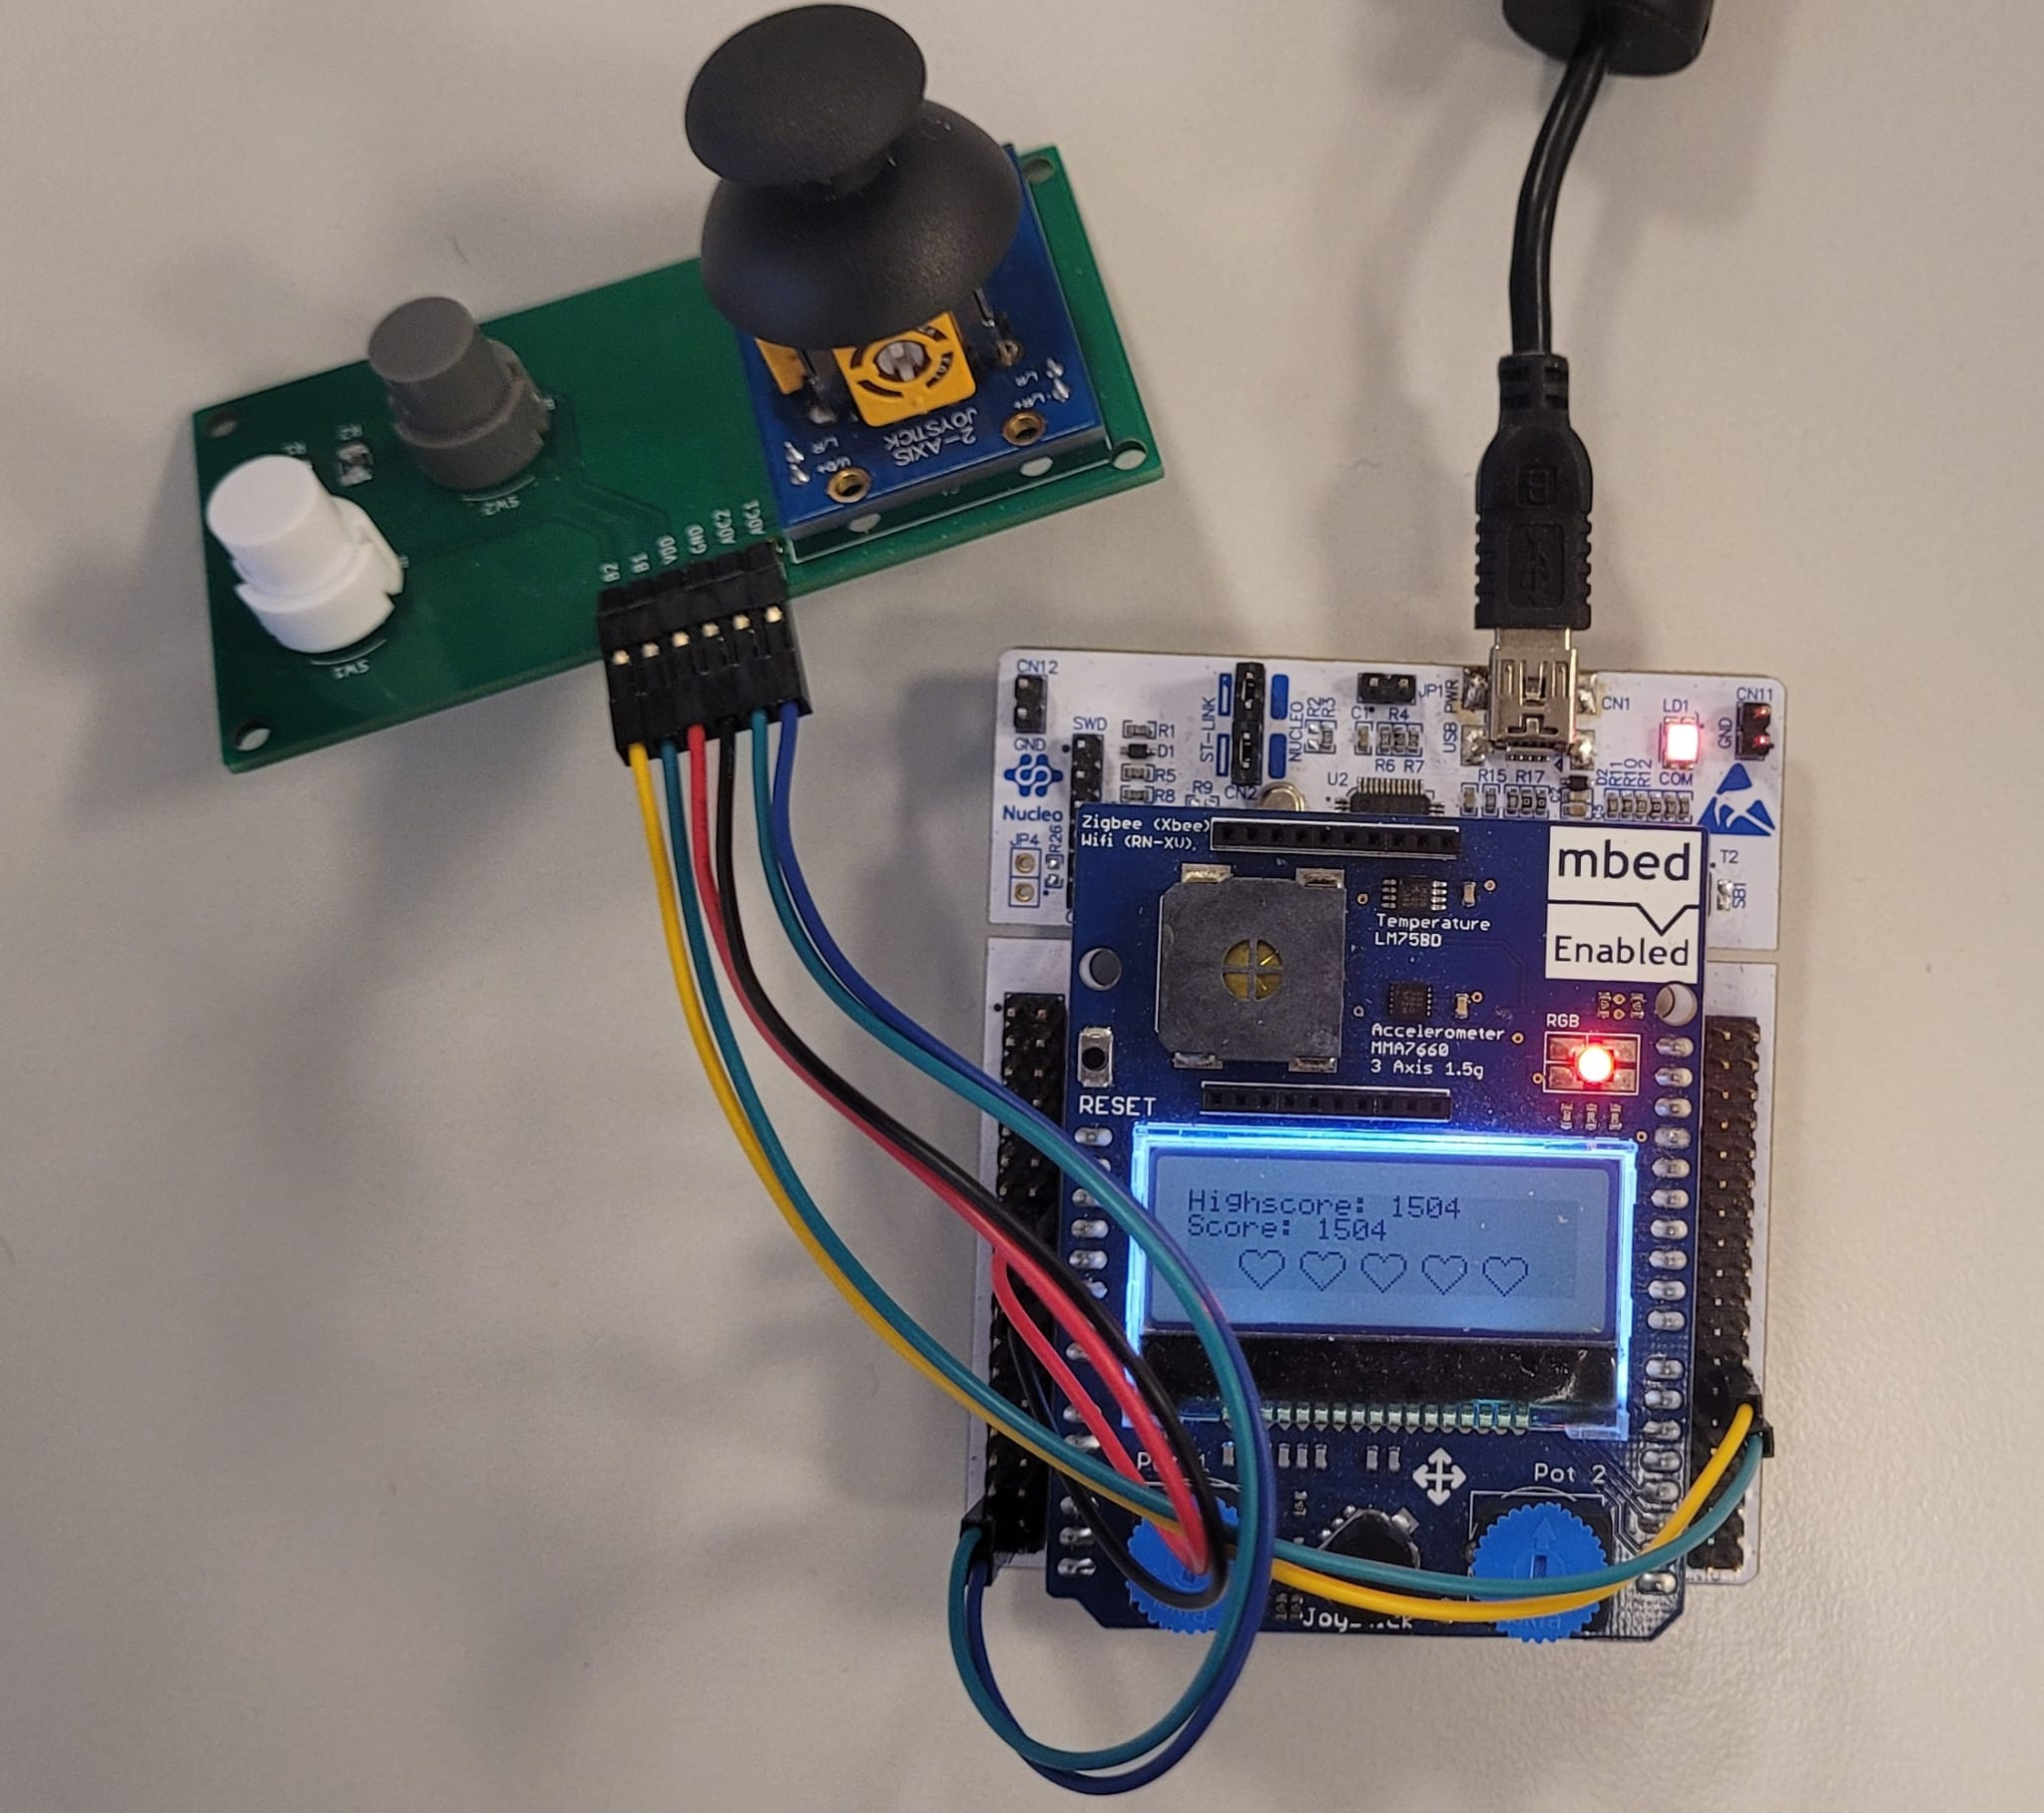
\includegraphics[height=16cm,keepaspectratio]{Picturs/spillet/WhatsApp Image 2026-01-23 at 14.22.54.jpeg}}; % CHANGE PHOTO ON THE FRONTPAGE HERE BY DEFINING A NEW FILEPATH
\end{tikzpicture}

\end{titlepage}

\pagecolor{white}
\newgeometry{top=2.81cm, bottom=2.75cm, outer=2.5cm, inner=3.5cm}
\pagestyle{empty}
\clearpage 
\section*{Abstrakt} 
\addcontentsline{toc}{section}{Abstrakt} 
\vspace{1em}

This report documents the design and implementation of an arcade inspired "endless runner" game, developed for the ARM Cortex-M4 CPU microcontroller using the STM32CubeIDE. The project emphasizes a modular software architecture, structured into the distinct layers: the Application Layer, the Application Interface Layer and the Hardware Abstraction Layer (HAL). This layerd appoach ensures code portability and maintainability by isolation hardware-specific drivers from the core game logic.

The game features an evolving difficulty system where gamplay speed and the players hitbox size increases over time. Technical implementation includes the use of fixed-point arithmetic for efficient physics calculations in a resource-constrained environment, as well as hardware timers (TIM2) to maintain a stable 30 Hz update frequency. Player-interaction is handled through a joystick and buttons, with visual feedback provided via an SPI-driven LCD and an RGB LED.

Key game mechanics such as collision detection, randomized projectile trajectories, and various power-ups (shields, score multipliers, and extra lives) were successfully integrated. The project demonstrates the successful synthesis of low-level hardware control and high-level software design, fulfilling the requirements for the 30010 Programming Project.

\vspace{15em}

\begin{figure}[h]
    \centering
    \begin{subfigure}{0.35\textwidth}
        
\includegraphics[width=\linewidth]{Picturs/signaturs/safija.jpeg}
        \caption{Safija Aagerup}
    \end{subfigure}
    \begin{subfigure}{0.42\textwidth}
        
\includegraphics[width=\linewidth]{Picturs/signaturs/image.png}
        \caption{William Riss}
    \end{subfigure}
\end{figure}

\begin{figure}[h]
    \centering
    \begin{subfigure}{0.45\textwidth}
        
\includegraphics[width=\linewidth]{Picturs/signaturs/nymand.png}
        \caption{Nikolaij Nymand}
    \end{subfigure}
    \begin{subfigure}{0.30\textwidth}
        
\includegraphics[width=\linewidth]{Picturs/signaturs/Daniel.jpg}
        \caption{Daniel Fenyvesi}
    \end{subfigure}
\end{figure}




\clearpage
\section*{Resume} 
\addcontentsline{toc}{section}{Resume} 
\vspace{1em}

Dette projekt dokumentere udviklingen at et funktionnelt arkadespil. Gennem projektet er der lagt vægt på at skabe en robust softwarearkitektur, der adskiller spil logik fra hardwarehåndtering, via en trelags model (application, Interface og HAL).

Det færdige system understøtter dynamisk sværhedsgrad og udnytter teknikker som fixed-point aritmetik og hardwaretimere for at opnå en stabil opdateringsfrekvens på 30 Hz, på trods af mikrocontrollerens begrænsede ressourcer. Spillet integrerer fuldt ud relevante perifere enheder, herunder joystick, LCD-display og RGB-LED.

Projektet demonstrerer en praktisk anvendelse af centrale elementer fra kursus 30010, såsom kollisionsdetektering, interrupt-håndtering og modulær programmering i C. Samlet set resulterer dette i et stabilt, udvideligt og veldokumenteret system, der lever op til samtlige opstillede designkrav.



\clearpage 
\tableofcontents
\clearpage 

% %  ======================================================
% % % MAIN SECTION
% %  ======================================================

\pagenumbering{arabic} % Definer at alle sider der kommer herefter skal markeres med arabiske tal 

\chapter{Introduktion} \label{chap:intro}

Indlejrede systemer spiller en central rolle i moderne teknologi og anvendes i mange felter såsom forbrugerelektronik og transportsystemer. Udvikling af software til mikrocontroller-baserede systemer kræver en velstruktureret og effektiv kode samt forståelse af tilhørende hardware, da ressourcer som hukommelse, energi og regnekraft er begrænsede. I 30010 Programmeringsprojekt kurset er formålet nemlig at arbejde med disse udfordringer gennem et design og implementering af et større softwareprojekt i C på en ARM-baseret mikrocontroller.

Dette programmeringsprojekt omhandler udviklingen af et arkadeinspireret spil med temaet SpaceShip. Det udarbejdes på en ARM Cortex-M4 mikrocontroller ved brug af STM32CubeIDE. Spillet simulerer en rumrejse hvor spilleren styrer en alien gennem et fjendtligt miljø med forskellige projektiler der skader spilleren undervejs, og spilleren kan påvirke potentialfeltet på disse. Undervejs håndterer spilleren begrænsede ressourcer, undgår forhindringer og forsøger at overleve skaden fra de forskellige projektiler af varierende type og skudvinkler.

Udover selve spilfunktionaliteten har projektet også et stærkt fokus på softwarearkitektur og især modularitet. Programmet er opdelt i tre lag: Application Layer, Application Interface Layer, og Hardware Abstraction Layer (HAL). Denne opdeling gør koden nemmere at genbruge, forstå og vedligeholde. Samtidig er der krav om dokumentation i form af flowcharts, block-diagrammer og modulbeskrivelser, hvilket hjælper med at sikre en struktureret tilgang til projektet.

Projektet bruger mange mikrocontroller-periferienheder, herunder GPIO, timere, interrupts, joystick, RGB-LED, LCD-display samt kommunikation vha. UART til en terminal på en computer. Numeriske beregninger vil være implementeret ved hjælp af fixed-point aritmetik, hvilket bruges og er nødvendigt i ressourcebegrænsede systemer.

Formålet med projektet er dermed ikke kun at udvikle et funktionelt spil, men også at vise, at vi kan håndtere hele processen fra idé til implementering.

Projektets overordnede rammer og krav er fastlagt i den udleverede projektbeskrivelse \cite{DTU30010ProjectDescription}. 
\clearpage 

\input{Chapters/02_blank.tex} 
\clearpage 

\chapter{Produkt Udvikling} \label{chap:ProduktUdvikling}

Ud fra de præsenterede udkast fra undervisningen har vi som gruppe valgt at udvikle et spil med udgangspunkt i en SpaceShip interstellar travel mission. 
På baggrund af de obligatoriske krav og forventninger, har vi analyseret de forskellige muligheder og herefter udvalgt en række minimumskrav, som danner fundamentet for spillets funktionalitet og design. Disse krav sikre at at vores projekt lever op til kursets læringsmål, samtidig med at de giver et godt fundament for videreudvikling af projektet. 
Vi har udvalgt følgende minimumskrav:

\section{Undervisningskrav} \label{chap:ProduktUdvikling_sec:MandatoryRequirement}
\vspace{0.5em}

\begin{itemize}
    \setlength{\itemsep}{5pt}
    \setlength{\parskip}{0pt}
    \setlength{\parsep}{0pt}
    \item Asteroids/planets with potential field effect (gravity, electric, magnetic, black hole or other)
    \item Game levels with increasing speed controlled by the timer/IRQ
    \item 3+ stages docked spaceship
    \item 3+ bullet types with 5+ shot angles
    \item Power-ups
    \item Number of lives on LCD and PC, number of points on LCD and PC, score / high score on LCD and PC
    \item Menu, help screen, and boss key
    \item Multiple bullets
    \item Random delta-angle
    \item Score / High score
    \item Show info on RGB LED
    \item Game controlled by 30010 joystick
    \item Partial/full game on the LCD
\end{itemize}

Med udgangspunkt i kursets obligatoriske krav herover samt den overordnede retning som vi ønsker at trække spillet hen imod, har vi lagt grundlaget for spillets funktionalitet og design. I denne proces har vi taget højde får både de tekniske rammer, der er sat af, den anvendt hardware, samt de læringsmål som projektet har til formå at opfylde.
I følgende afsnit uddybes først de yderligere kravspecifikationer, som vi selv har defineret på baggrund af den idé vi har visualiseret \ref{chap:ProduktUdvikling_sec:VoresKrav}.
Herefter præsenteres spillets overordnede formål og opbygning \ref{chap:ProduktUdvikling_sec:VoresSpil}. 

\vspace{10em}

\section{Kravspecifikationer og implementering} \label{chap:ProduktUdvikling_sec:VoresKrav}
\vspace{0.5em}

For at sikre, at ovenstående krav realiseres i praksis, har vi defineret konkrete kravspecifikationer og tilhørende implementeringsmetoder:

\textbf{Stigende hastighed over tid}
\\Spillets sværhedsgrad øges gradvist ved, at den overordnede spil-hastighed forøges mellem faste tidsintervaller. Dette er implementeret ved hjælp af en timer, som efter hvert interval øger bevægelseshastigheden spillets elementer, hvilket skaber en naturlig stigning i sværhedsgraden.

\textbf{Ændring af spillerens størrelse (Docked spaceship)}
\\Spillerens figur ændres gradvist størrelse i takt med spillets progression. Dette medfører også en stigende sværhedsgrad, da spilleren får mindre manøvrerum. 

\textbf{Power-ups}
\\Der er implementeret flere typer power-ups, som midlertidigt ændrer spillets dynamik. Power-ups vises tilfældigt i spillet og aktiveres ved kollision med spilleren.
\vspace{-0.5em}
\begin{itemize}
    \setlength{\itemsep}{0pt}
    \setlength{\parskip}{1pt}
    \setlength{\parsep}{0pt}
    \item Heart powerup: giver spilleren et ekstra liv
    \item Forcefield powerup: giver spilleren imunitet for projektilerne i 10 sekunder
    \item Multiplier powerup: spilleren vil optjene 2x point de følgende 10 sekunder
\end{itemize}

\textbf{Projektil typer og randomiseret skudretning}
\\Spillet indeholder flere typer projektiler med forskellig hastighed, størrelse og skade. Projekternes skudretning genereres tilfældigt indenfor et defineret vinkelinterval på 60 grader, hvilket bidrager til variation og uforudsigelighed i gameplayet.
\vspace{-0.5em}
\begin{itemize}
    \setlength{\itemsep}{0pt}
    \setlength{\parskip}{1pt}
    \setlength{\parsep}{0pt}
    \item Regular Bullet: mellem fart, mellem hitbox, tager 1 liv
    \item Cannonball: langsom fart, stor hitbox, tager 2 liv
    \item Bouncing Bullet: mellem fart, mellem hitbox, tager 1 liv, hopper tilbage på skærmens top og bund
\end{itemize}

\textbf{Menu og boss key}
\\Spillet indeholder en startmenu med adgang til hjælpeskærm, mulighed for at afslutte spillet og vigtigst af alt, starte spillet. Derudover er der implementeret en boss-key, som giver spilleren mulighed for at pause eller forlade spillet på ethvert tidspunkt.

\textbf{Visuel feedback via RGB LED}
\\RGB LED’en viser spillerens status, hvilket giver hurtig og intuitiv visuel feedback til brugeren. 
\vspace{-0.5em}
\begin{itemize}
    \setlength{\itemsep}{0pt}
    \setlength{\parskip}{1pt}
    \setlength{\parsep}{0pt}
    \item Rød: flasher 0.5 sec efter man mister et liv
    \item Grøn: tændt, men i hviletilstand
\end{itemize}

\textbf{Input via joystick og knapper}
\\Spilleren styrer figuren ved brug af joysticket på NUCLEO boardet (ved at trykke ned på det). Samme joystick bruges til at manøvre gennem menuen og starte spillet. 30010 joysticket vil blive brugt til at "styre" projektilernes bevægelse.

\textbf{Visning af spilinformation på LCD}
\\Liv, score og highscore opdateres løbende på LCD-displayet og i Putt-terminalen, så spilleren har fuldt overblik over spillets tilstand til enhver tid.

\vspace{5em}

\section{Aim of the game} \label{chap:ProduktUdvikling_sec:VoresSpil}
\vspace{0.5em}

Vores spil er opbygget som en "travel mission", med det formål at udforske en mystisk og fremmed planet ude i rummet. Det er et "endless runner game", hvor spilleren forsøger at nå så langt som muligt.
Spilleren bevæger sig op og ned, ved brug af et joystick. Når joysticket holdes ned, bevæger spillerens figur sig op, og ellers bliver figuren trukket ned af planetens tyngdefelt. 
Under spillet bliver der skudt projektiler (bullets) rundt, som spillerne skal undgå. Hvis spilleren bliver ramt, mister man liv afhængigt af typen af bullet. Når spilleren ikke har flere liv tilbage, afslutter spillet. 
Sværhedsgraden i spillet stiger løbende i forhold til tid, dette vil blive gjort ved at implementere flere bullets på hvert level. Tempoet vil sigt samt størrelsen på spilleren, hvilket vil gøre det svære at manøvrere rundt.
For at hjælpe spilleren på vej er der implementere forskellige typer af powerups som vil kunne blive aktiveret løbende.
Spillet fortsætter i et uendeligt loop, indtil spilleren mister alle sine liv, eller vælger at forlade spillet.

\begin{figure}[h]
    \centering    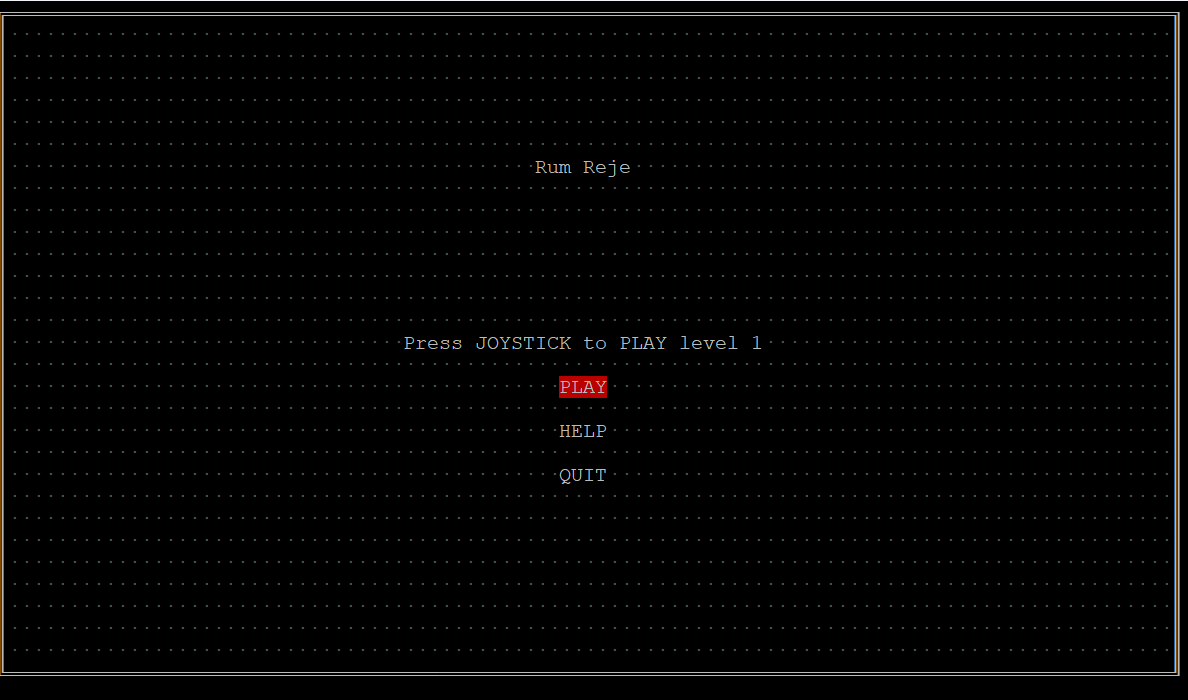
\includegraphics[width=0.74\textwidth]{Picturs/spillet/Screenshot1.png}
    \caption{Billed af spillets "Home screen"}
    \label{fig:spil_billed_1}
\end{figure}
\vspace{-1em}
\begin{figure}[h]
    \centering    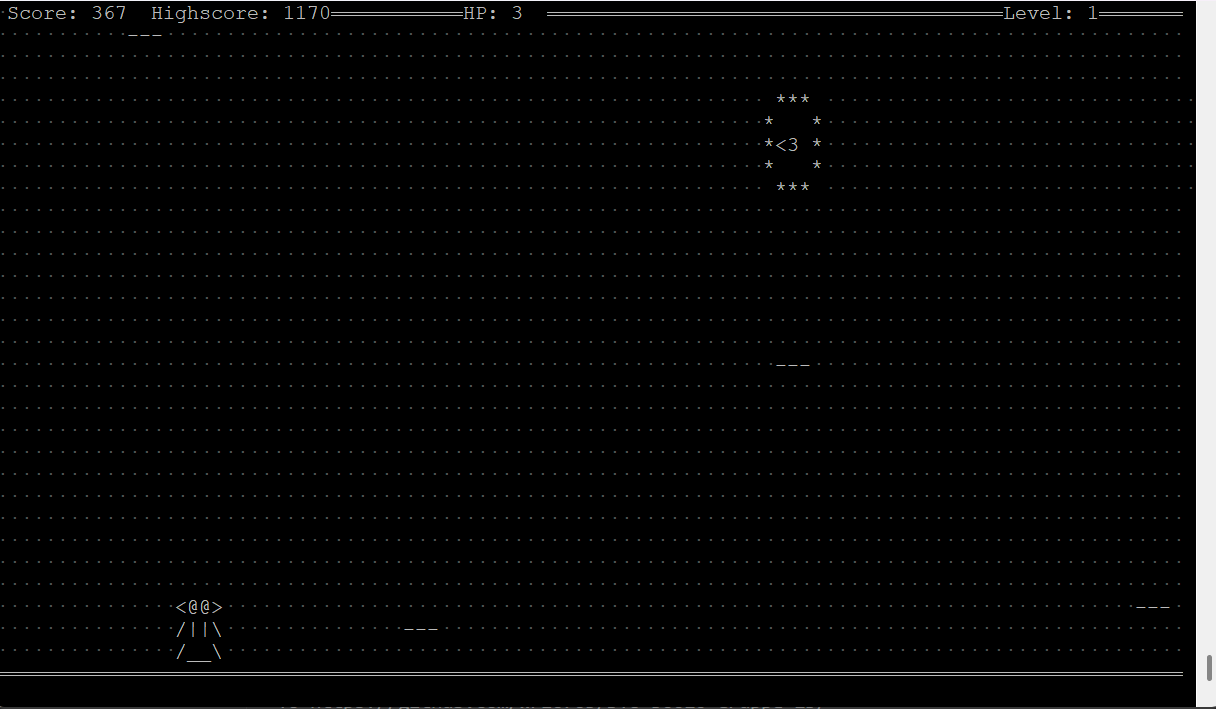
\includegraphics[width=0.74\textwidth]{Picturs/spillet/Screenshot2.png}
    \caption{Billed midt spil}
    \label{fig:spil_billed_2}
\end{figure}
\vspace{-1em}


På figur \ref{fig:spil_billed_1} ses spillets menu. Spilleren kan vælge mellem 3 muligheder. "HELP", som vil føre til en ny side, hvor spilleren kan lærer om reglerne for spillet. "PLAY" som vil starte spillet og "QUIT" som vil forlade spillet.
På figur \ref{fig:spil_billed_2} kan der ses et billede af hvordan spillet ser ud midt-game. Scoren, highscore, liv og level kan ses i toppen af skærmen. Spillerens figur kan ses nede i venstre hjørne og en health powerup kan spottes oppe til venstre. 


\section{Block diagram} \label{chap:ProduktUdvikling_sec:BlockDiagram}
\vspace{0.5em}

For at give et samlet overblik over spillets opbygning og interne struktur er der blevet udarbejdet et blockdiagram. Som illustrerer den overordnede organisering af systemet. Diagrammet repræsenterer projektets overordnet filstruktur og viser samtidigt hvordan spillets funktionalitet er opdelt i separate filer og moduler. Hver block i diagrammet svarer til en central del af koden og afspejler ansvarsfordelingen i projektet.  

\vspace{1em}

\begin{figure}[h]
    \centering    
    
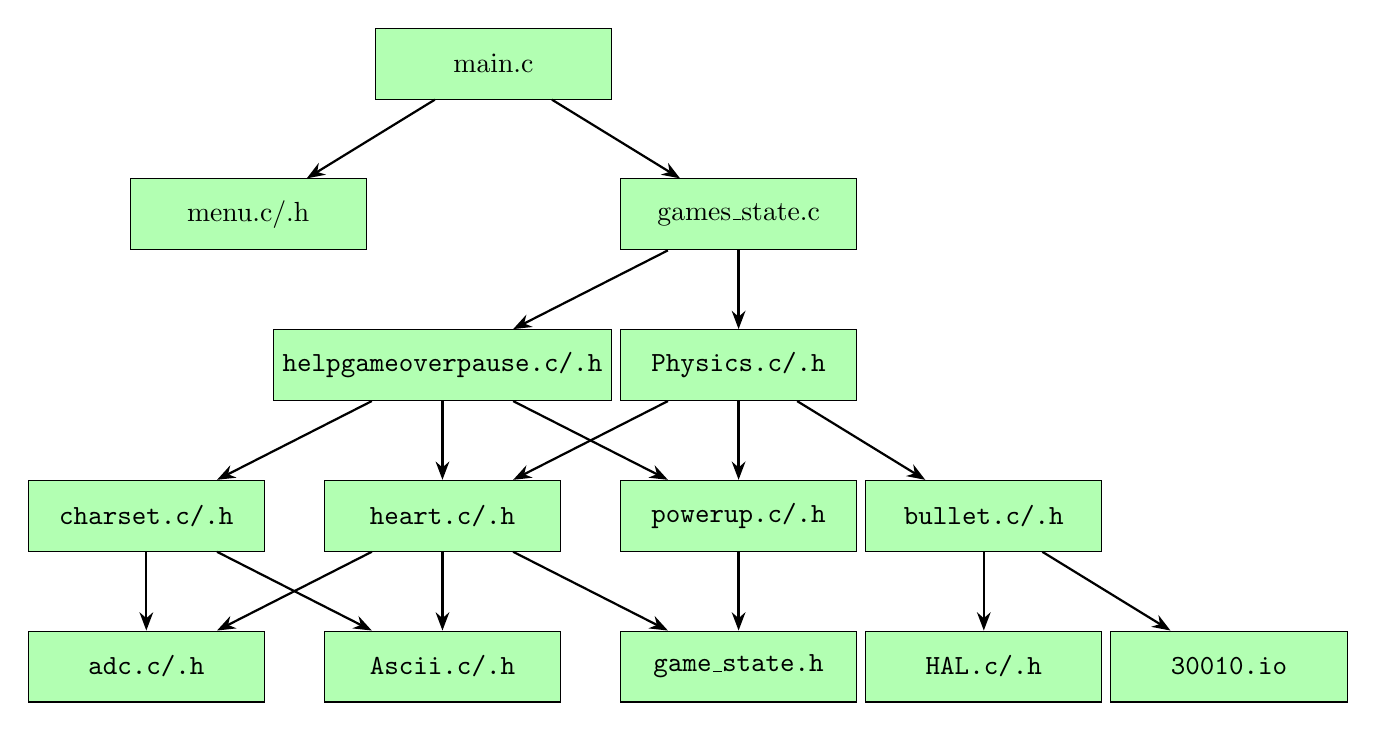
\begin{tikzpicture}[
    box/.style={
        draw,
        rectangle,
        minimum width=3cm,
        minimum height=0.9cm,
        fill=green!30,
        align=center
    },
    arrow/.style={
        -Stealth,
        thick
    },
    node distance=1cm and 0.1cm
]

% Top
\node[box] (main) {main.c};

% Level 2
\node[box, below left =of main] (menu) {menu.c/.h};
\node[box, below right=of main] (gamestate) {games\_state.c};

\draw[arrow] (main) -- (menu);
\draw[arrow] (main) -- (gamestate);

% Level 3
\node[box, below left=of gamestate] (help) {\texttt{helpgameoverpause.c/.h}};
\node[box, below =of gamestate] (physics) {\texttt{Physics.c/.h}};

\draw[arrow] (gamestate) -- (help);
\draw[arrow] (gamestate) -- (physics);

% Level 4
\node[box, below left=of help] (charset) {\texttt{charset.c/.h}};
\node[box, below=of help] (heart) {\texttt{heart.c/.h}};

\node[box, below=of physics] (powerup) {\texttt{powerup.c/.h}};
\node[box, below right=of physics] (bullet) {\texttt{bullet.c/.h}};
\draw[arrow] (help) -- (charset);
\draw[arrow] (help) -- (heart);

\draw[arrow] (physics) -- (powerup);
\draw[arrow] (physics) -- (bullet);
\draw[arrow] (physics) -- (heart);
\draw[arrow] (help) -- (powerup);


% Level 5
\node[box, below=of charset] (adc) {\texttt{adc.c/.h}};
\node[box, below=of heart] (ascii) {\texttt{Ascii.c/.h}};
\node[box, below=of powerup] (gamestateh) {\texttt{game\_state.h}};
\node[box, below=of bullet] (hal) {\texttt{HAL.c/.h}};
\node[box, right=of hal] (io) {\texttt{30010.io}};
\draw[arrow] (charset) -- (adc);
\draw[arrow] (heart) -- (ascii);
\draw[arrow] (powerup) -- (gamestateh);
\draw[arrow] (bullet) -- (hal);
\draw[arrow] (bullet) -- (io);
\draw[arrow] (heart) -- (gamestateh);
\draw[arrow] (heart) -- (adc);
\draw[arrow] (charset) -- (ascii);

\end{tikzpicture}
    \caption{Udkast til block diagram}
    \label{fig:blokdiagram}
\end{figure}

Block diagrammet her over viser den hierarkiske opbygning af projektets filer og den overordnede afhængighed mellem de enkelte moduler. Øverst i diagrammet ses main.c, som fungere som programmets indgangspunkt og koordinere den overordnede afvikling af spillet. Herfra fordeles kontrollen til central styringsmoduler som menu.c og game\_state.c, der håndtere bruger interaktionen samt skiftet mellem spillets forskellige tilstande. 
De under lignende moduler varetager afgrænsede funktioner såsom spilfysik, spilletilstande og positions bestemmelse, mens de nederste moduler hovedsaligt står for input, output og direkte kommunikation med den underliggende hardware. Denne struktur illustrere en klar adskillelse mellem spillets logik og hardwareafhængige funktioner, og danner grundlaget for software arkitekturen, som vi vil komme ind på i næste afsnit.

\vspace{15em}

\section{Software Architecture} \label{chap:ProduktUdvikling_sec:SoftwareArchitecture}
\vspace{0.5em}

Systemet er opdelt i tre lag: et Application Layer, et Application Interface Layer samt et Hardware Abstraction Layer (HAL). Denne lag deling danner grundlaget for en overskuelig opbygning af spillet og sikrer en klar adskillelse mellem spillets regler og den tekniske hardware håndtering.

\begin{figure}[h]
    \centering    
    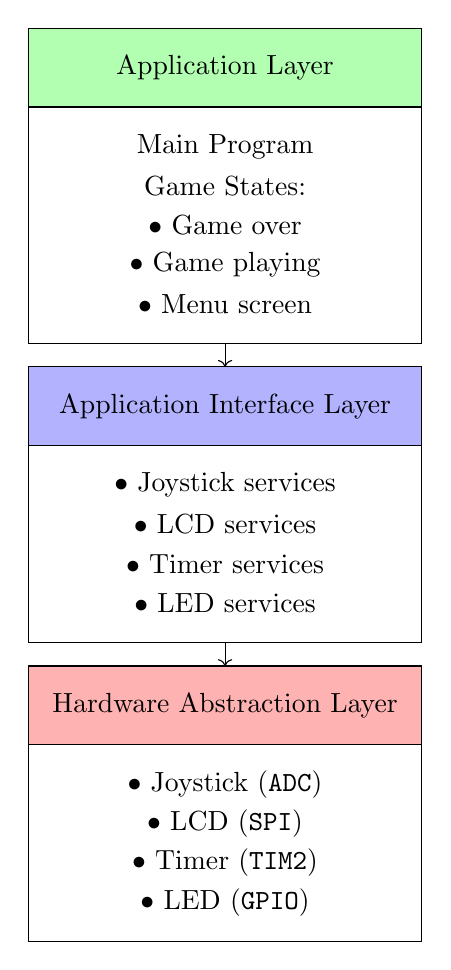
\begin{tikzpicture}
  %first box
  \draw[fill=green!30] (0,0) rectangle (5,-1);
  \draw (0,-1) rectangle (5,-4);
  \draw[->] (2.5,-4) -- (2.5,-4.3);
  %second box
  \draw[fill=blue!30] (0,-4.3) rectangle (5,-5.3);
  \draw (0,-5.3) rectangle (5,-7.8);
  \draw[->] (2.5,-7.8) -- (2.5,-8.1); 
  %third box
  \draw[fill=red!30] (0,-8.1) rectangle (5,-9.1);
  \draw (0,-9.1) rectangle (5,-11.6);


  %titles
  \node at (2.5,-0.5) {Application Layer};
  \node at (2.5,-4.8) {Application Interface Layer};
  \node at (2.5,-8.6) {Hardware Abstraction Layer}; 

  %text in application layer
  \node at (2.5,-1.5) {Main Program};
  \node at (2.5,-2) {Game States:};
  \node at (2.5,-2.5) {$\bullet$ Game over};
  \node at (2.5,-3) {$\bullet$ Game playing};
  \node at (2.5,-3.5) {$\bullet$ Menu screen};
  %text in application interface layer
  \node at (2.5,-5.8) {$\bullet$ Joystick services};
  \node at (2.5,-6.3) {$\bullet$ LCD services};
  \node at (2.5,-6.8) {$\bullet$ Timer services};
  \node at (2.5,-7.3) {$\bullet$ LED services};
  %text in hardware abstraction layer
  \node at (2.5,-9.6) {$\bullet$ Joystick (\texttt{ADC})}; 
  \node at (2.5,-10.1) {$\bullet$ LCD (\texttt{SPI})};
  \node at (2.5,-10.6) {$\bullet$ Timer (\texttt{TIM2})};
  \node at (2.5,-11.1) {$\bullet$ LED (\texttt{GPIO})};  



\end{tikzpicture}
    \caption{Software Architecture diagram}
    \label{fig:Software_arkitektur}
    \vspace{0em}
\end{figure}

\subsection{Application Layer}
Dette lag indeholder spillets overordnede logik og styring. Laget håndterer den overordnede spille logik, samt de forskellige spilde tilstande som, Home Screen, Game Play og Game Over. Laget her er uafhængigt af det underliggende hardware og fokuserer udelukkende på spillets overordnede adfærd og regler.

\textbf{Game Context:} 
Centralt for dette lag er en GameContext struktur (struct), der fungere som spillets hukommelse. Den holder styr på variabler som game\_state, level, score og Highscore.

\textbf{Game State:}
Laget bestemmer hvilket tilstand spilet er i. Altså om systemet skal eksekverer logikken for menuen, selve gameplayet eller hjælpeskærmen. Dette er med til at sikre aspillet reagere korrekt på de logiske overgange.

\textbf{Physics \& Rules:} 
Her beregnes de matematiske regler for spillet, såsom projektil-baner og spillerens bevægelse. Baseret på det data som der bliver leveret fra de underliggende lag. 

\subsection{Application Interface layer}
Laget her fungerer som et bindende lag mellem spillets logik og den underliggende hardware. Det sørger for, at data flyder flydende mellem lagene, men dets primære formål er at gøre koden “portabel”. Dette lag fungerer som "oversætteren" og det afgørende bindeled mellem spillets logik og den specifikke hardware. Ved at isolere de hardware definerede funktioner i dette lag, kan Application Layer i princippet flyttes til en anden platform, uden at spillets kernelogik skal omskrives.

\subsection{Abstraction Layer}
Dette lag indeholder de hardware specifikke funktioner. 
Hardware-delen fokuserer på de moduler, der interagerer direkte med mikrokontrolleren og de eksterne komponenter på 30010-boardet. Dette lag danner fundamentet for systemet ved at transformere fysiske signaler til data så softwaren kan modtage input og give feedback.
Laget sørger for direkte kommunikation med hardwaren og stiller simple funktioner til rådighed for de overliggende lag. 

\textbf{Input-håndtering (Joystick \& Knapper):} 
Som vist i flowchartet afhænger spillets forløb af brugerens input. Her implementeres funktioner til at aflæse de analoge værdier fra joysticket via ADC’en (Analog-to-Digital Converter) samt de digitale input fra knapperne. Disse værdier normaliseres, så spillogikken let kan beregne bevægelse.

\textbf{Visuel Output (LCD \& RGB LED):} 
Denne del af koden styrer opdateringen af LCD-displayet via SPI-kommunikation. RGB LED’en styres her for at give øjeblikkelig feedback på spillerens tilstand, så som tab af liv eller opsamling af power-ups.

\textbf{Timing og Afbrydelser (Timer):} 
For at sikre en stabil spilhastighed benyttes hardware-timere. Dette gør det muligt at opdatere spillets tilstand med en fast frekvens (30 Hz), hvilket er essentielt for en flydende spiloplevelse.

Denne software arkitektur er afgørende for projektets samlede robusthed og skalerbarhed. Ved, konsekvent, at adskille hardware abstraktionerne fra spillets regler, sikres en struktur hvor fejlfinding bliver væsentligt lettere, da problemet kan isoleres til specifikke lag uden at påvirke hele systemet. Det gør det muligt at udvikle spillets individuelle funktioner, samtidig med at det holder koden struktureret og læselig.

\section{Systemets overordnede opbygning} \label{chap:ProduktUdvikling_sec:overordnet opbygning}
\vspace{0.5em}

\subsection{Flow diagram af spillet} \label{chap:ProduktUdvikling_sec:flowchart}

\begin{figure}[H]
    \centering
    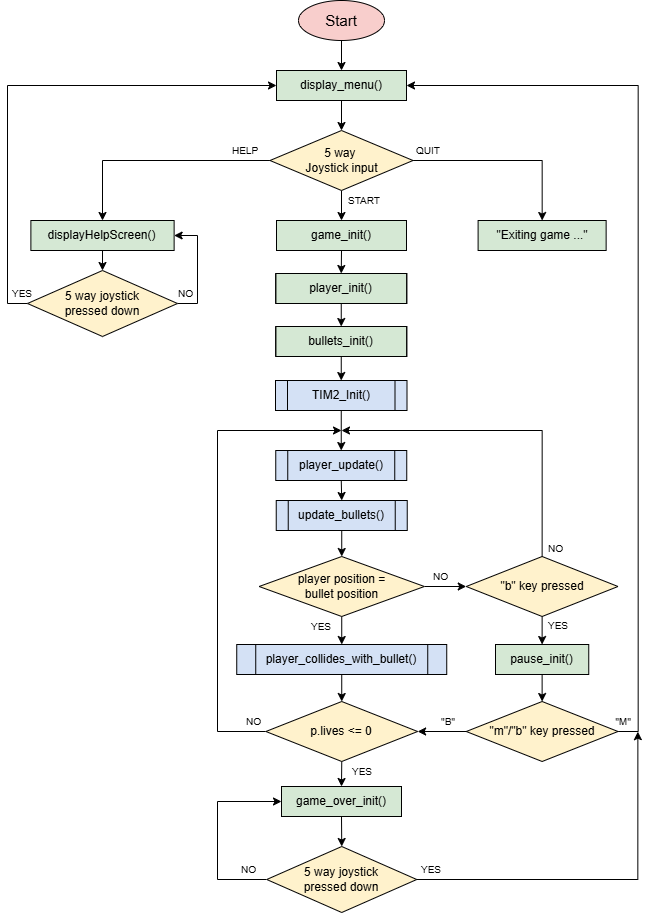
\includegraphics[width=\textwidth]{Picturs/Diagrammer/FINAL_FLOW_FARVER_10000.drawio.png}
    \caption{Flow diagram af vores spil}
    \label{fig:flow_diagram}
\end{figure}

Repræsenteret herover ses et overordnet flowdiagram af vores spil (figur \ref{fig:flow_diagram}). Diagrammet er opbygget efter klassiske flowdiagram-principper, hvor beslutningspunkter anvendes til at håndtere bruger input, og procesbokse beskriver de handlinger og funktioner som systemet udfører. I grøn er initialisering af visuelle output repræsenteret og i blå er spillets fundamentale funktion, som vil blive uddybet følgende (afsnit \ref{chap:ProduktUdvikling_sec:tid&spiller}).

Programmet starter med visning af menuen (\lstinline!display_menu()!), hvor spilleren ved hjælp af et "5-way" joystick kan vælge mellem 3 forskellige muligheder. Afhængigt af det valgte input fortsætter programmet enten til hjælpeskærmen (\lstinline!displayHelpScreen()!), initialisering af spillet (\lstinline!game_init()!) eller afslutning af programmet. 
Når spillet starter initialiseres de nødvendige spilleelementer, herunder spiller (\lstinline!player_init()!) projektiler (\lstinline!bullets_init()!) og timer (\lstinline!TIM2_init()!). Efterfølgende indgår programmet i et opdaterende loop, hvor spillerens og projektilernes tilstand opdateres (\lstinline!player_update()! \& \lstinline!update_bullets()!) og hver der kontinuerligt kontrolleres for kollision mellem disse to (\lstinline!player_collides_with_bullet()!). Under spillet er der mulighed for at pause spillet (\lstinline!pause_init()!) ved hjælp at et tast input. Her har spilleren mulighed mellem at genoptage spillet eller returner til menuen. Spillet fortsætter til alle liv er brugt op, og vil initialisere en game over skærm (\lstinline!game_over_init()!) der vil fremvise spillerens score og highscore, og give spilleren mulighed for at returnere til menuen. 

For at give et mere detaljeret indblik i spillets funktionalitet fokuserer det følgende afsnit på de centrale processer i spillets opdateringsloop. Her uddybes håndteringen af spilleren og projektilernes positioner samt den anvendte kollisionslogik, da disse funktioner er afgørende for spillets interaktion og dynamik.

\vspace{0.5em}
\subsection{level system \& spillerens position} \label{chap:ProduktUdvikling_sec:tid&spiller}
\vspace{0.5em}

\begin{figure}[H]
    \centering
    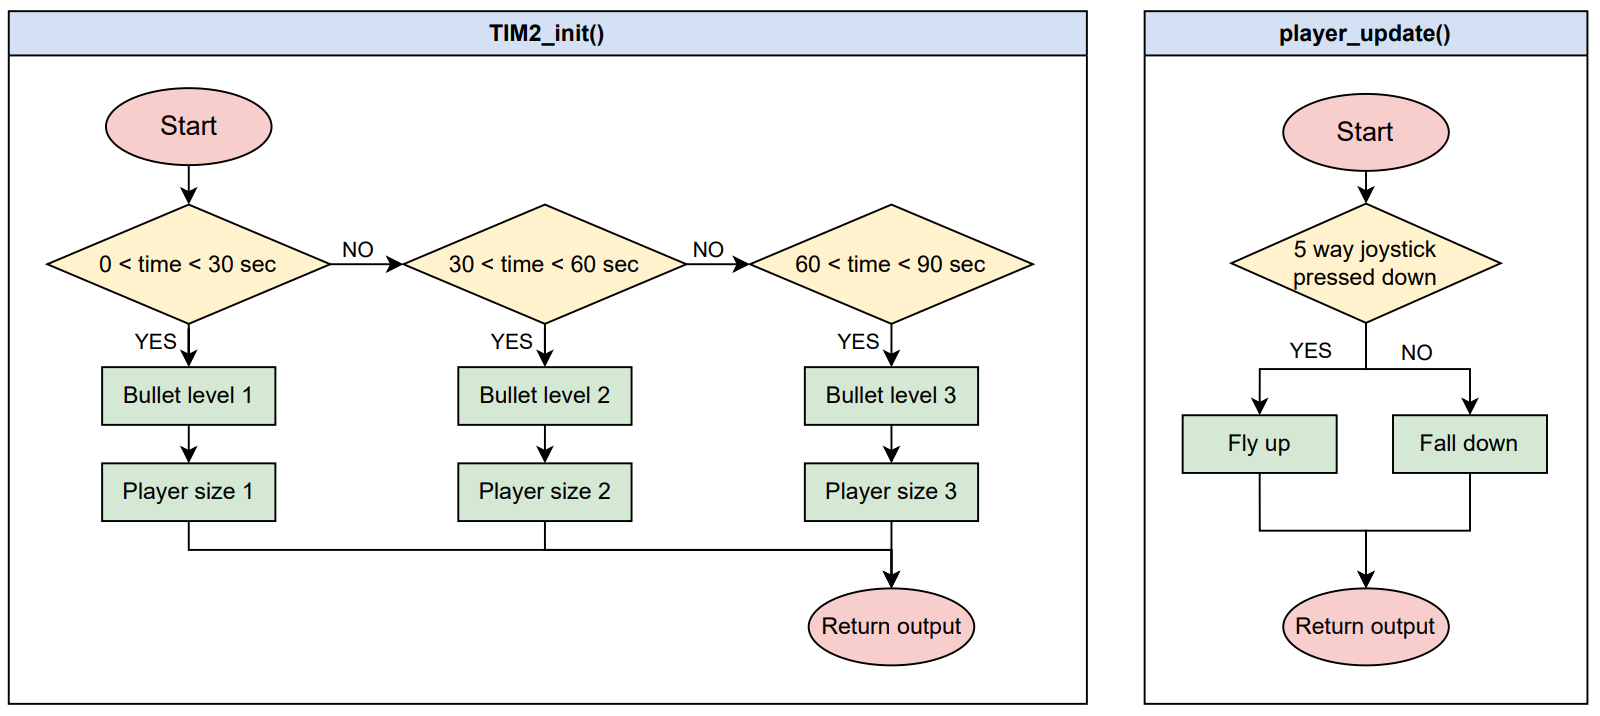
\includegraphics[width=\textwidth]{Picturs/Diagrammer/FINAL_FR_TIM_PLAYER.png}
    \caption{Flow diagram af TIM2\_init() \& player\_update()}
    \label{fig:TIME_PLAYER}
\end{figure}
\vspace{-2.5em}

Som illustreret i \lstinline!player_update()! diagrammet i figur \ref{fig:TIME_PLAYER}, er spillerens position afhængig af det input joysticket modtager. Hvis joysticket holdes ned vil karakteren bevæge sig opad og ellers vil den falde ned, som følge af spillets bevægelseslogik. Denne mekanisme er med til at sikre at spilleren kontinuerligt skal interager for at opretholde en stabil position. 

Som tidligere sagt er sværhedsgraden tidsbaseret, det er lige ledes illustrerede i figur \ref{fig:TIME_PLAYER} med \lstinline!TIM2_init()!. Her bruges en timer til at opdele spillet i forskellige tidsintervaller. Hvor projektil niveauet gradvis stiger, samt størrelsen på spilleren, hvilket vil gøre det sværere at undgå projektilerne. 

\subsection{Bullet position \& liv update} \label{chap:ProduktUdvikling_sec:skud_og_liv}
\vspace{0.5em}

\begin{figure}[H]
    \centering
    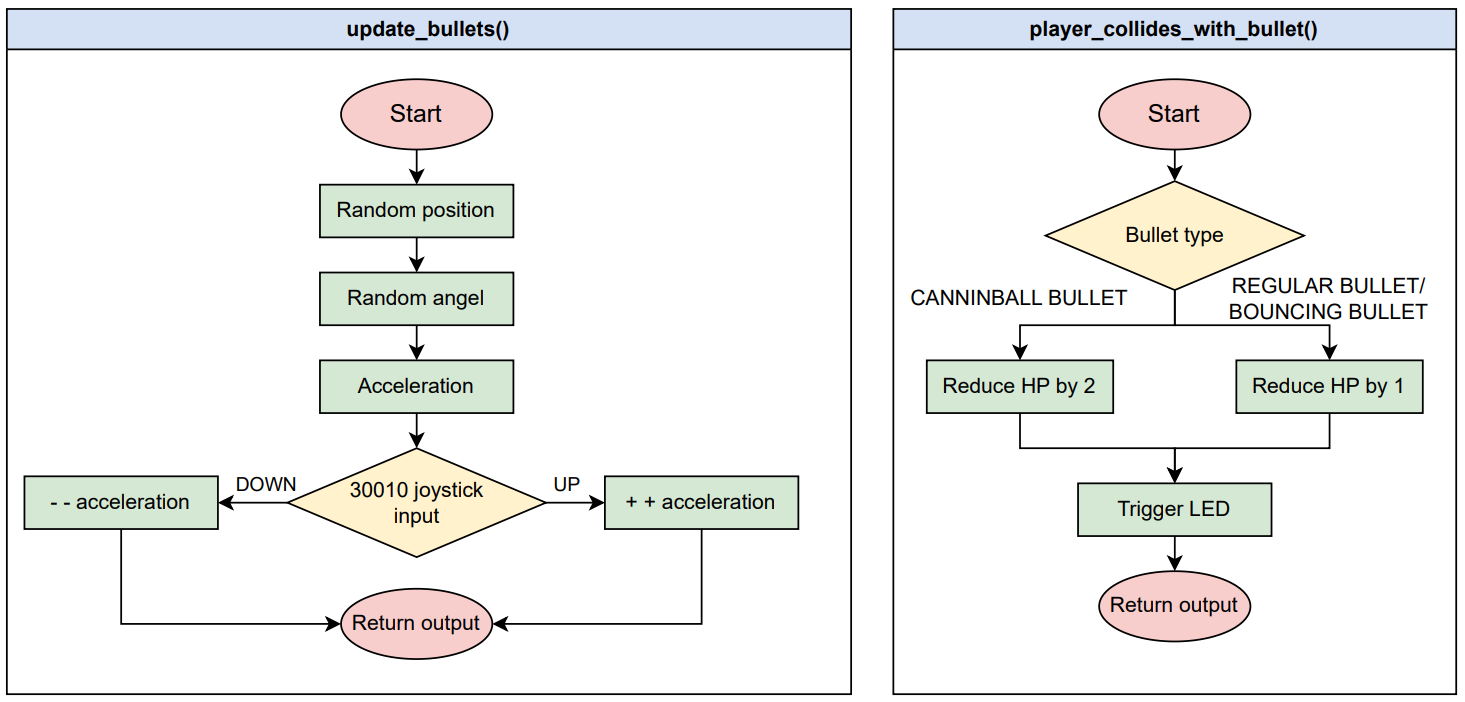
\includegraphics[width=\textwidth]{Picturs/Diagrammer/BULLRT_DIAGRAM.png}
    \caption{Flow diagram af update\_bullets() \& player\_collides\_with\_bullet()}
    \label{fig:bullet_live}
\end{figure}
\vspace{-2.5em}

For at håndtere projektiler og interaktionen med spillerne, benyttes funktionen \lstinline!update_bullets()! og \lstinline!player_collides_with_bullet()!. Som det fremgår i figur \ref{chap:ProduktUdvikling_sec:skud_og_liv}, gennemløber programmet alle aktive projektiler i hvert frame. Her opdateres projektilets position baseret på dets gældende hastighed og acceleration. En serlig feature i vores spil er at projektilernes acceleration styres af hardwaren, vha. et 30010 joystick.
Her gang et projektil opdateres, tjekkes der for kollision med spilleren. hvis spillerens koordinater overlapper med et projektil, vil spilleren mindste liv afhængig ag hvilke bullet type de har ramt. Ved kollision, aktiveres LED'en på hardwaren og giver spilleren et øjeblikkelig feedback på skaden.

\vspace{0.5em}
\subsection{Power ups} \label{chap:ProduktUdvikling_sec:powerups}
\vspace{0.5em}

På samme må måde som \lstinline!player_collides_with_bullet()! opfang om spilleren kolliderer med bullets bliver det også taget stilling til om der er kontakt med "powerups". Systemet sørge automatisk for at der med jævne mellemrum dukker power ups op på skærmen. De bevæger sig fra højre mod venstre, og spilleren skal aktivt navigere hen mod dem for at opsamle dem. Der findes tre forskellige typer. Når spilleren opsamler en power up aktivere det en specifik effekt. Hvor "liv" giver et ekstra liv, er de to andre tidsbaseret. Det betyder at spilleren kun har fordelen i et kort tidsrum, før spilleren vender tilbage til normal tilstand. Gennemgangen af disse afsnit viser, hvordan spillet er bygget op af forskellige moduler, der hver især har et specifikt ansvar. Ved at kombinere spillerens bevægelser, projektilernes baner og de taktiske fordele fra power-ups, skabes et sammenhængende spilsystem. 
\clearpage

\chapter{Projekt struktur} \label{chap:analyse}

For at realisere de opstillede krav og den beskrevne softwarearkitektur, er projektet opdelt i en hardware orienteret del og en software orienteret del. Dette sikrer en klar adskillelse mellem lavniveaus-drivere og den overordnede spillogik. Det er her de fysiske input transformeres til data, som spillets logik kan reagere på.




\section{Hardware Abstraction layer (HAL)} \label{chap:Projektstruktur_sec:hardwere}
\vspace{0.5em}

\vspace{3pt}
\subsection{Timer}
\vspace{3pt}

Spillet har sin egen timer indbygget via STM-mikrocontrolleren. 

\vspace{1em}
\begin{lstlisting}
     RCC->APB1ENR |= 0x00000001;
	    TIM2->PSC = 6399; 
	    TIM2->ARR = 332;   
	    TIM2->CNT = 0x0000;  
	    TIM2->DIER = 0x0001;
	    TIM2->CR1 = 0x0001; 
        NVIC->ISER[0] = 0x10000000; 
	    NVIC->IP[28] = 0x10;
\end{lstlisting}
\vspace{-2em}

Koden foroven er en liste af "indstillinger" som timeren indholdet. \lstinline!APB1ENR! indeholder initieringen for timeren, hvor LSB indeholder skal være hot for aktiveringen af \lstinline!TM2!. \lstinline!PSC! indeholder prescaleren som er justeret til 30 hz. \lstinline!ARR! indeholder autoreload, samt \lstinline!CNT! som resetter vores \lstinline!TIM2!-timer. \lstinline!DIER! undersøger hvorledes en opdatering forekommer. 

\vspace{3pt}
\subsection{joystick-input}
\vspace{3pt}

Et simpelt joystick input for MBED, til det tilsvarende bitværdier for hhv. op, ned og knappen (center). Koden indencere bittet ud fra hvilket input den får.

\vspace{1em}
\begin{lstlisting}
    RCC->AHBENR |= RCC_AHBPeriph_GPIOB;
    GPIOB->MODER &= ~(0x3 << (5 * 2));   
    GPIOB->PUPDR &= ~(0x3 << (5 * 2));
    GPIOB->PUPDR |=  (0x2 << (5 * 2)); 
\end{lstlisting}
\vspace{-2em}

Koden forover indencere hex-tallet for at give en byte-række one-hot kodet, så rækkens indencering svarer til et return på indencering af bit-stringen. Dette gør det nemt at overfører joystick-input til eventuelle if-statements i andre filer via et function-call.

\vspace{1em}
\begin{lstlisting}
     return (GPIOB->IDR & (1 << 5)) ? 1 : 0;
\end{lstlisting}
\vspace{-2em}

Som ser sådanne ud, altså et simpelt ternary statement, hvis 1, returner 1, hvis 0 returner 0. Man kun undre sig over hvorfor man ikke bare kan returnere selve værdien for \lstinline!GPIOB!, men et function call acceptere kun en conditional.

\vspace{3em}

\vspace{3pt}
\subsection{LCD}
\vspace{3pt}

Der benyttes en 128x32 monokrom dot matrix LCD skærm til at visualisere spillets gang. Skærmen styres gennem en Serial Peripheral Interface (SPI) bus, som transmitterer data en byte af gangen. Da hver pixel på skærmen kun kræver en bit (tændt eller slukket), opdeler man skærmen i 512 grupper af 8 vertikale pixels. Dette betyder at en byten der sendes til skærmen opdatere en vertikal stribe på 8 pixels, hvilket optimere opdateringen på displayet. For at styre denne software benytter vi en skærm buffer (\lstinline!unit8_t lcd_buffe[512]!), som fungere som et lokalt kort over skærmes pixels. 
For at visualisere spildata som score og liv, har vi implementerede et brugerdefineret tegnsæt (\lstinline!character_data!). Her er hvert tegn defineret som en 5 byte matrix, der repræsentere bogstavets form.
Funktionerne \lstinline!lcd_write_string! tager en tekststreng og mapper den direkte til bufferen. Alle ændringer (score opdatering, liv opdatering og spille graftik) skrives først til \lstinline!lcd_buffer!, for at sikre en stabil fremvisning. Når alle beregningerne er færdige kaldes \lstinline!lcd_commit!, som skubber hele bufferen til den fysiske skærm ved hjælp af \lstinline!lcd_push_buffer!. Dette sikre at spilleren altid ser et komplet og opdateret billede. 
På samme måde som teksten bliver opdateret på skærmen bliver spillerens liv også displayet derpå, dog ud fra et \lstinline!tom_heart_data! og \lstinline!full_heart_data! i stedet.




\section{Application Layer} \label{chap:Projektstruktur_sec:softwere}
\vspace{0.5em}

\vspace{3pt}
\subsection{overall spil-mekanikker}
\vspace{3pt}

Spillet er opsat sådan, at over tid, spillerkarakteren (typisk referes i koden som \lstinline!ALIEN!)  udvikler sig større, dermed en større hitbox, hvilket essentiel gør spillet sværere, da bevægelseshastigheden ikke ændres, så man som spiller er nødt til at kunne reagere hurtigere på skud. der findes et mere spil mekanik, der øger vanskeligheden af spillet. 3 muligheder for at forøge sin scorer i form af "powerups". Skrevet i koden som \lstinline!!

\vspace{3pt}
\subsubsection{Gravity}
\vspace{3pt}

Der er implementeres en accelererede tyngdekraft på spiller-spriten, som konstant trækker spilleren ned mod "gulvet". siden spillet kører med et begrænse antal karakterer, samt et konstant antal pladser på vores 100x32 grid, skal 

\vspace{1em}
\begin{lstlisting}
    void update_player(player *p, uint8_t joystick){.
        p->score += 1;
        p->vy += p->ay;
        p->y += p->vy;
        if (p->y < Y_MIN + 256){
		      p->y = Y_MIN + 256;
		      p->vy = 0;  
        }
	    else if (p->y > Y_MAX - 512){
		      p->y = Y_MAX - 512;
		      p->vy = 0;
	    }
    }
\end{lstlisting}
\vspace{-2em}

Dette beskriver tyngdekraftens virkning på spilleren. \lstinline{Y_MIN} defineres med pointeren \lstinline!p! for structen \lstinline!Player!, som konstant ændre hastigheden af faldet, pr ændring i position, som essentielt er et konstant accelererende legeme uden en begrænsning, men siden skærmen forudsager, at spiller-karakteren opnår så høj en hastighed, virker løsningen fint til lejligheden. En aktiv tyngdekraft er et af 

\vspace{3pt}
\subsubsection{Sprites}
\vspace{3pt}

Når der omtales sprites, menes der bevægelige figurer som f.eks. Player-karateren, der består af mere end én karakter. dette er mere af den "front-end" mæssige aspekter af projektet. 

\vspace{1em}
\begin{lstlisting}
    static const char level1[ALIEN_HEIGHT_LVL_1][ALIEN_WIDTH +1] = {
	"<@@>",
	"/||\\",
	"/__\\"
	};
\end{lstlisting}
\vspace{-2em}

koden forover et eksempel på en af projektets sprites. En spiller-karakter, der flyttes med brugerens input via joystick. Spriten er ikke konstant, da den ændret 2 gange til en større figur




\section{Prioriteret funktioner}
\vspace{0.5em}

Denne sektion fokusere på en række udvalgte funktioner, som vi mener har en høj relevans for sammensætningen af spillet, samt noget interessant at sige om den individuelle funktion.

\vspace{3pt}
\subsection{Gameloop}
\vspace{3pt}

Kan findes i \lstinline!game_state.c!, Denne funktion virker som primus motor for hele spillets gentagende processor, som looper i timerens 30 Hz. Funktionen er kun kaldt en gang i \lstinline!game_state_update! i samme fil. 

\vspace{1em}
\begin{lstlisting}
    ctx->timer_counter++;

    if(ctx->timer_counter > 2700){
        ctx->timer_counter = 1800;
    }
    if(ctx->timer_counter % 900 == 0){
        if(ctx->level < 3){
            ctx->level++;
            bullets_set_max(ctx, &bullet_system); 
        }
    }
\end{lstlisting}
\vspace{-2em}

Første del af funktionen ser man \lstinline!TIM2!-timeren gå op 30 gange i sekundet, hvor første if statement bestemmer overflow, siden timeren er en 30, har vi et reset 900 pr level, så counter ikke bliver for høj, men stadig viser den rigtige værdi. Næste if-statement bestemmer efter 900 iterations, som på 30 Hz vil være 30 sekunder, at \lstinline!ctx->level! øges med 1. Resten af funktionen kører en masse andre funktioner, der er med til at få hele spillet til at virke.

\vspace{3pt}
\subsection{Menu Update}
\vspace{3pt}

Kan findes i \lstinline!menu.c!. Denne funktion det første man møder, når man kører spillet. Den initialisere logikken for menuen og læner sig meget op af Hardware abstraction layer, da den kommunikere med \lstinline!HAL.c!, for at få inputtet fra onboard joystick, som opdatere switch casen \lstinline!menu_mode!, inden i \lstinline!GameContext!-structen, som kan findes i \lstinline!game_state.h!.

\vspace{3em}
\begin{lstlisting}
if (ctx->menu_mode == MENU_MODE_PLAY && ctx->game_state == GAME_STATE_MENU) {
    printf("\x1B[%d;%dH\033[41mPLAY\033[0m",(h/2)+2,(w/2)-2); 
    printf("\x1B[%d;%dHHELP",(h/2)+4,(w/2)-2);
    printf("\x1B[%d;%dHQUIT",(h/2)+6,(w/2)-2);
}
else if (ctx->menu_mode == MENU_MODE_HELP && ctx->game_state == GAME_STATE_MENU) {
    printf("\x1B[%d;%dHPLAY",(h/2)+2,(w/2)-2);
    printf("\x1B[%d;%dH\033[41mHELP\033[0m",(h/2)+4,(w/2)-2);
    printf("\x1B[%d;%dHQUIT",(h/2)+6,(w/2)-2);
}
else if (ctx->menu_mode == MENU_MODE_QUIT && ctx->game_state == GAME_STATE_MENU) {
    printf("\x1B[%d;%dHPLAY",(h/2)+2,(w/2)-2);
    printf("\x1B[%d;%dHHELP",(h/2)+4,(w/2)-2);
    printf("\x1B[%d;%dH\033[41mQUIT\033[0m",(h/2)+6,(w/2)-2);
}
\end{lstlisting}
\vspace{-2em}

Koden forover laver en meget simpel og rekursiv opdatering i ANSI-print via if-else statements, der fortæller brugeren hvilket menu type, der er valgt, ved at highlighte menutypen i rød.

\vspace{3pt}
\subsection{Bullet system}
\vspace{3pt}

Dette er en serie af funktioner, som for det meste kan findes \lstinline!bullets.c! og \lstinline!Physics.c!, funktionen \lstinline!spawn_simple_bullet!, gør nemlig det som navnet antager, den sætter skuddene ind på skærmen i tilfældigt position, langs y-aksen (\lstinline!DISPLAY_HEIGHT!), som ud fra en simpel indbygget \lstinline!rand()!-funktion. positionen bliver sat på y-aksen således: \lstinline!b->y = (2 + rand() % (DISPLAY_HEIGHT - 4)) << 8;!, så skuddene bliver sat tilfældigt, men undgår at clippe igennem skærmens grænser. Grunden til at \lstinline!DISPLAY_HEIGHT! bliver left-shifted med 8, er fordi den blev right-shifted med 8 tidligere i koden. Skuddene panere så fra højreside af skærmen, og ikke nok med at spawn-placering er tilfældig, vinkel fra hvor de skydes er også tilfældig ud fra en -30$^{\circ}$ til 30$^{\circ}$ begrænsning. Koden for dette er skrevet således:\\
\lstinline!b->angle = (rand() % 61) - 30;!\\
\lstinline!angle!, som er indenunder \lstinline!bullet!-type structen, tager et tilfældigt nummer, som modulus af 61 giver en arbitrer værdi der sætter linær funktion som hvor skuddet eksempelvis flytter sig 1 nedad, efter den normalt vil flyttes sig 3 til venstre. Siden spillet er opbygget sådan, at 30010 joysticket ændrer accelerationen og dermed hastigheden af skuddene.\\

\begin{lstlisting}
    if(screen_y < 2) {
        bs->bullets[i].vy = -bs->bullets[i].vy;
        bs->bullets[i].y = 2 << 8;
    } else if(screen_y > (DISPLAY_HEIGHT - 2)) {
        bs->bullets[i].vy = -bs->bullets[i].vy;
        bs->bullets[i].y = (DISPLAY_HEIGHT - 2) << 8;
    }
\end{lstlisting}
\vspace{-2em}

Her er en funktion, der nok virker bekendt, da den beskriver type 2 skuddene (\lstinline!bs->bullets[i].type == 2)!), som mere eller mindre samme måde som kursets 'bouncing ball'-øvelse fra de tidligere dage. Dog er der få ændringer, f.eks. kan \lstinline!BULLET_TYPE_BOUNCE! kun "hoppe" fra de to horisontale side af skærmen, og forsvinder (\lstinline!bs->bullets[i].alive=0!), når den rammer et af de to vertikale sider af skærmen. Inden i funktionen \lstinline!update_bullets!, kører dette stykke kode helt i starten.\\

\begin{lstlisting}
    if(bs->bullets[i].alive){
        bs->bullets[i].x += bs->bullets[i].vx;
        bs->bullets[i].y += bs->bullets[i].vy;
        bs->bullets[i].vx += bs->bullets[i].ax;
        bs->bullets[i].vy += bs->bullets[i].ay;
        if(player_collides_with_bullet(&p, &bs->bullets[i])){
            if (bs->bullets[i].type == BULLET_TYPE_CANNON) {
                p.hp -= 2;
            } else {
                p.hp -= 1;
    }
\end{lstlisting}
\vspace{-2em}

Her ses mekanismen, der får spillet til reelt at blive et spil og ikke bare en simulation. Siden PVP mekanismen blev indført, har hvert skud nu en opdaterende acceleration fra spawn-punktet. Det vil sige at ikke nok med at hastighen pr. skud-type, ændres, men også den "nye" hastigheden bliver bestemt ud fra \lstinline!bs->bullets[i].ax!, som er styret af bruger-input.

\vspace{3pt}
\subsection{Powerup}
\vspace{3pt}

Powerup-systemet er implementeret for at give spilleren midlertidige fordele og skabe variation i gameplayet. Systemet er opbygget som en del af Application Layer og interagerer med spiller-structen (player) samt den overordnede spiltilstand (GameContext), og er tidsbaseret.

Systemet understøtter tre forskellige powerups:

\begin{itemize}
    \setlength{\itemsep}{0pt}
    \setlength{\parskip}{3pt}
    \setlength{\parsep}{0pt}
    \item Heart (heal) - genskaber 2 liv for spilleren
    \item Multiplier - fordobler spillerens score i en begrænset periode
    \item Forcefield - afbøjer fjendtlige projektiler omkring spilleren
\end{itemize}

Alle powerups er repræsenteret som separate instanser af Powerup-structen inde i player-structen, hvilket sikrer, at der maksimalt kan eksistere én aktiv powerup af hver type ad gangen.

Hver powerup er repræsenteret ved en \texttt{Powerup}-struct som indeholder tilstands- og positionsdata såsom om den er aktiv, type, position, hastighed samt forrige position. Dette gør det muligt at behandle powerups på samme måde som øvrige objekter der bevæger sig i spillet og genbruge eksisterende logik for bevægelse, kollision og tegning.

Spawn af powerups styres i funktionen \texttt{spawn\_powerup()} og er direkte afhængig af spillets interne timer (\texttt{ctx->timer\_counter}), som opdateres i gameloopet med 30 Hz. Spawn logikken bruger modulus-operatoren til at fordele powerups jævnt over tid:\\

\begin{lstlisting} 
void spawn_powerup(player *p, GameContext *ctx) {
    uint32_t t = ctx->timer_counter;

   if ((t+600) % 900 == 0 && !p->heart_pickup.active) {
        p->heart_pickup.active = 1;
        p->heart_pickup.type = POWERUP_HEART;
        p->heart_pickup.x = DISPLAY_WIDTH << 8;
        p->heart_pickup.y = 5 << 8;
        p->heart_pickup.vx = -128;
        p->heart_pickup.vy = 0;
    }
\end{lstlisting}
\vspace{-2em}

Ved at forskyde timer-værdien med 600 opnås løbende spawning af powerups inden for samme 900-tick interval (svarer til 30 sekunder).

Alle powerups spawner i højre side af skærmen (\texttt{DISPLAY\_WIDTH << 8}) og bevæger sig vandret mod venstre med konstant hastighed.

Opdatering af powerups sker i funktionen \texttt{powerups\_Update()}, som følger samme overordnede struktur som andre bevægelige objekter i spillet. Først slettes tidligere tegnede positioner, derefter opdateres positionen, hvorefter kollision og redraw bliver kørt:\\

\begin{lstlisting} 
if (p->heart_pickup.active) {
        p->heart_pickup.prev_x = p->heart_pickup.x;
        p->heart_pickup.prev_y = p->heart_pickup.y;
        p->heart_pickup.x += p->heart_pickup.vx;
        p->heart_pickup.y += p->heart_pickup.vy;
\end{lstlisting}
\vspace{-2em}

Hvis en powerup bevæger sig uden for skærmens grænser deaktiveres den automatisk:\\

\begin{lstlisting} 
if ((p->heart_pickup.x >> 8) < 0 || (p->heart_pickup.x >> 8) >= DISPLAY_WIDTH ||
        (p->heart_pickup.y >> 8) < 0 || (p->heart_pickup.y >> 8) >= DISPLAY_HEIGHT) {
        p->heart_pickup.active = 0;
    }
\end{lstlisting}
\vspace{-2em}

Kollision mellem spiller og powerups kontrolleres eksplicit for hver type af powerup. Ved kollision mellem disse to deaktiveres poweruppen, og den tilhørende effekt aktiveres:\\

\begin{lstlisting} 
if (p->heart_pickup.active && heal_collides_with_player(p)) {
        p->heart_pickup.active = 0;
        powerup_heal_player(p);
    }
\end{lstlisting}
\vspace{-2em}

Effekterne initialiseres i separate funktioner for at bevare modularitet i systemet der køres i projektet. Eksempelvis bliver score-multiplieren initialiseret således:\\

\begin{lstlisting} 
void powerup_score_multiplier_init(player *p) {
            p->score_multiplier = 2;
            p->multiplier_active = 1;
            p->multiplier_timer = 300;
}
\end{lstlisting}
\vspace{-2em}

Forcefield-poweruppen er anderledes fra de øvrige ved at direkte kunne påvirke fjendtlige projektiler frem for selve spilleren. I funktionen \texttt{powerup\_forcefield\_apply()} beregnes vektoren mellem spillerens center og projektilets center. Hvis projektilet befinder sig inden for en fast defineret radius, påføres en acceleration væk fra spilleren i samme retning som den ankom med:\\

\begin{lstlisting} 
    float dx_pix = dx_fixed / 256.0f;
    float dy_pix = dy_fixed / 256.0f;
    float dist = sqrtf(dx_pix * dx_pix + dy_pix * dy_pix);
\end{lstlisting}
\vspace{-2em}

Retningsvektoren normaliseres og accelerationen skaleres ud fra afstanden fra projektilet til spilleren, hvilket vil give en naturlig afbøjning.
Resultatet konverteres tilbage til 8.8 fixed-point formattet:\\

\begin{lstlisting} 
    int ax_fixed = (int)(nx * strength_pixels * 256.0f);
    int ay_fixed = (int)(ny * strength_pixels * 256.0f);
    b->ax += ax_fixed;
    b->ay += ay_fixed;
\end{lstlisting}
\vspace{-2em}



\section{Structs}
\vspace{0.5em}

\vspace{3pt}
\subsection{Player}
\vspace{1em}

    \begin{lstlisting} 
typedef struct player {
    int16_t x, y, vy, ay;
    int16_t score, score_multiplier, highscore;
    int16_t width, height;
    int16_t prev_x, prev_y;
    uint8_t hp;
    uint8_t alien_level;

    Powerup heart_pickup;
    Powerup forcefield_pickup;
    Powerup multiplier_pickup;

	uint16_t forcefield_active;
	uint16_t multiplier_active;	
	uint16_t forcefield_timer;
	uint16_t multiplier_timer;

	uint16_t led_timer;

} player;
    \end{lstlisting}
\vspace{-2em}

Denne struct indeholder alle variabler der hyppigt bruges når mekanikker der påvirker spiller bliver skrevet. Dette setup definerer en form for attributter for structens navn, og gør det nemt at anvende de samme variabler i andre funktioner og andre file med includes.


\vspace{3pt}
\subsection{Gamecontext}
\vspace{3pt}

\lstinline!GameContext!-structen er simpel nok. Denne struct fungerer som den centrale samling af alle tilstande for spillet, som skal være tilgængeligt på tværs af filer og funktioner. Structen bruges til at styre spillets tilstand, menu-navigation, tid og niveau-logik og fungerer som ledet mellem hardware input og applikationslaget.

Herunder ses et udsnit af vores \texttt{game\_state.h}-kode. 

\vspace{1em}
 \begin{lstlisting}
typedef struct {
    uint8_t game_state;
    uint8_t menu_mode;
    uint8_t prev_joystick;
    uint8_t prev_sw1;
    uint32_t timer_counter;
    uint8_t level;
    uint32_t highscore;
    int16_t joy_ax;
    int16_t joy_ay;
    int16_t joy_x; 
    int16_t joy_y;

} GameContext;
 \end{lstlisting}
\vspace{-2em}

 Spillets generelle flow styres vha. variablen \texttt{game\_state} som styrer hvilket logiske forløb der udføres i \texttt{game\_state\_update()}, fx. menu, om spillet er aktivt, pause eller game over. Menu-navigation håndteres vha. \texttt{menu\_mode}.

 Logikken for tid er samlet i variablen \texttt{timer\_counter} som stiger med én for hver iteration af gameloopet. Denne variabel bruges til styring af niveau-progression, powerup-spawns samt andre tidsafhængige mekanikker. For eksempel øges spillets sværhedsgrad for hvert 900. tick, som svarer til 30 sekunder.

 Variablen \texttt{level} bestemmer spillets aktuelle sværhedsgrad og bliver blandt andet brugt til den dynamiske ændring af antallet af aktive projektiler. Highscoren gemmes i \texttt{highscore}.

 Joystickets position gemmes i værdierne \texttt{joy\_x} og \texttt{joy\_y} samt de tilhørende accelerationsværdier \texttt{joy\_ax} og \texttt{joy\_ay}, i GameContext. Ved at gemme disse værdier i GameContext holdes inputaflæsningen adskilt fra bevægelsen af spilleren. 
\clearpage 

\chapter{Brugermanual} \label{chap:Brugermanual}

Dette afsnit fungere som en vejledning til opsætning og anvendelse af spillet. Projektet er opbygget som et sammenspil mellem software og hardware, hvor begge dele afhænger af hinanden for at fungere som ønsket.
Inden spillet kan spilles, skal de nødvendige software indstillinger konfigureres. Herunder valg af input, kalibrering samt de korrekte forbindelser mellem applikationen og de fysiske komponenter. Disse indstillinger er med til at sikre, at spillet kan modtage og fortolke dataet fra hardwaren på en sikker og ensartet måde. 
For at opnå dette kræves der en række forberedende trin, som gennemgås i de følgende underafsnit.

\section{Hardware konfiguration} \label{chap:Brugermanual_sec:hardwear}
\vspace{0.5em}

For at køre spillet skal følgende hardware-komponenter andvendes:

\begin{itemize}
    \setlength{\itemsep}{4pt}
    \setlength{\parskip}{0pt}
    \setlength{\parsep}{0pt}
    \item NUCLEO-F302R8 mikrokontroller
    \item MBED Extension board (monteret direkte på Nucleo-boardet)
    \item 30010 Joystick (med tilhørende knapper)
    \item USB kabel
    \item Computer med USB port
\end{itemize}

\begin{figure}[h]
    \centering
    \begin{minipage}{0.33\textwidth}
        \centering
        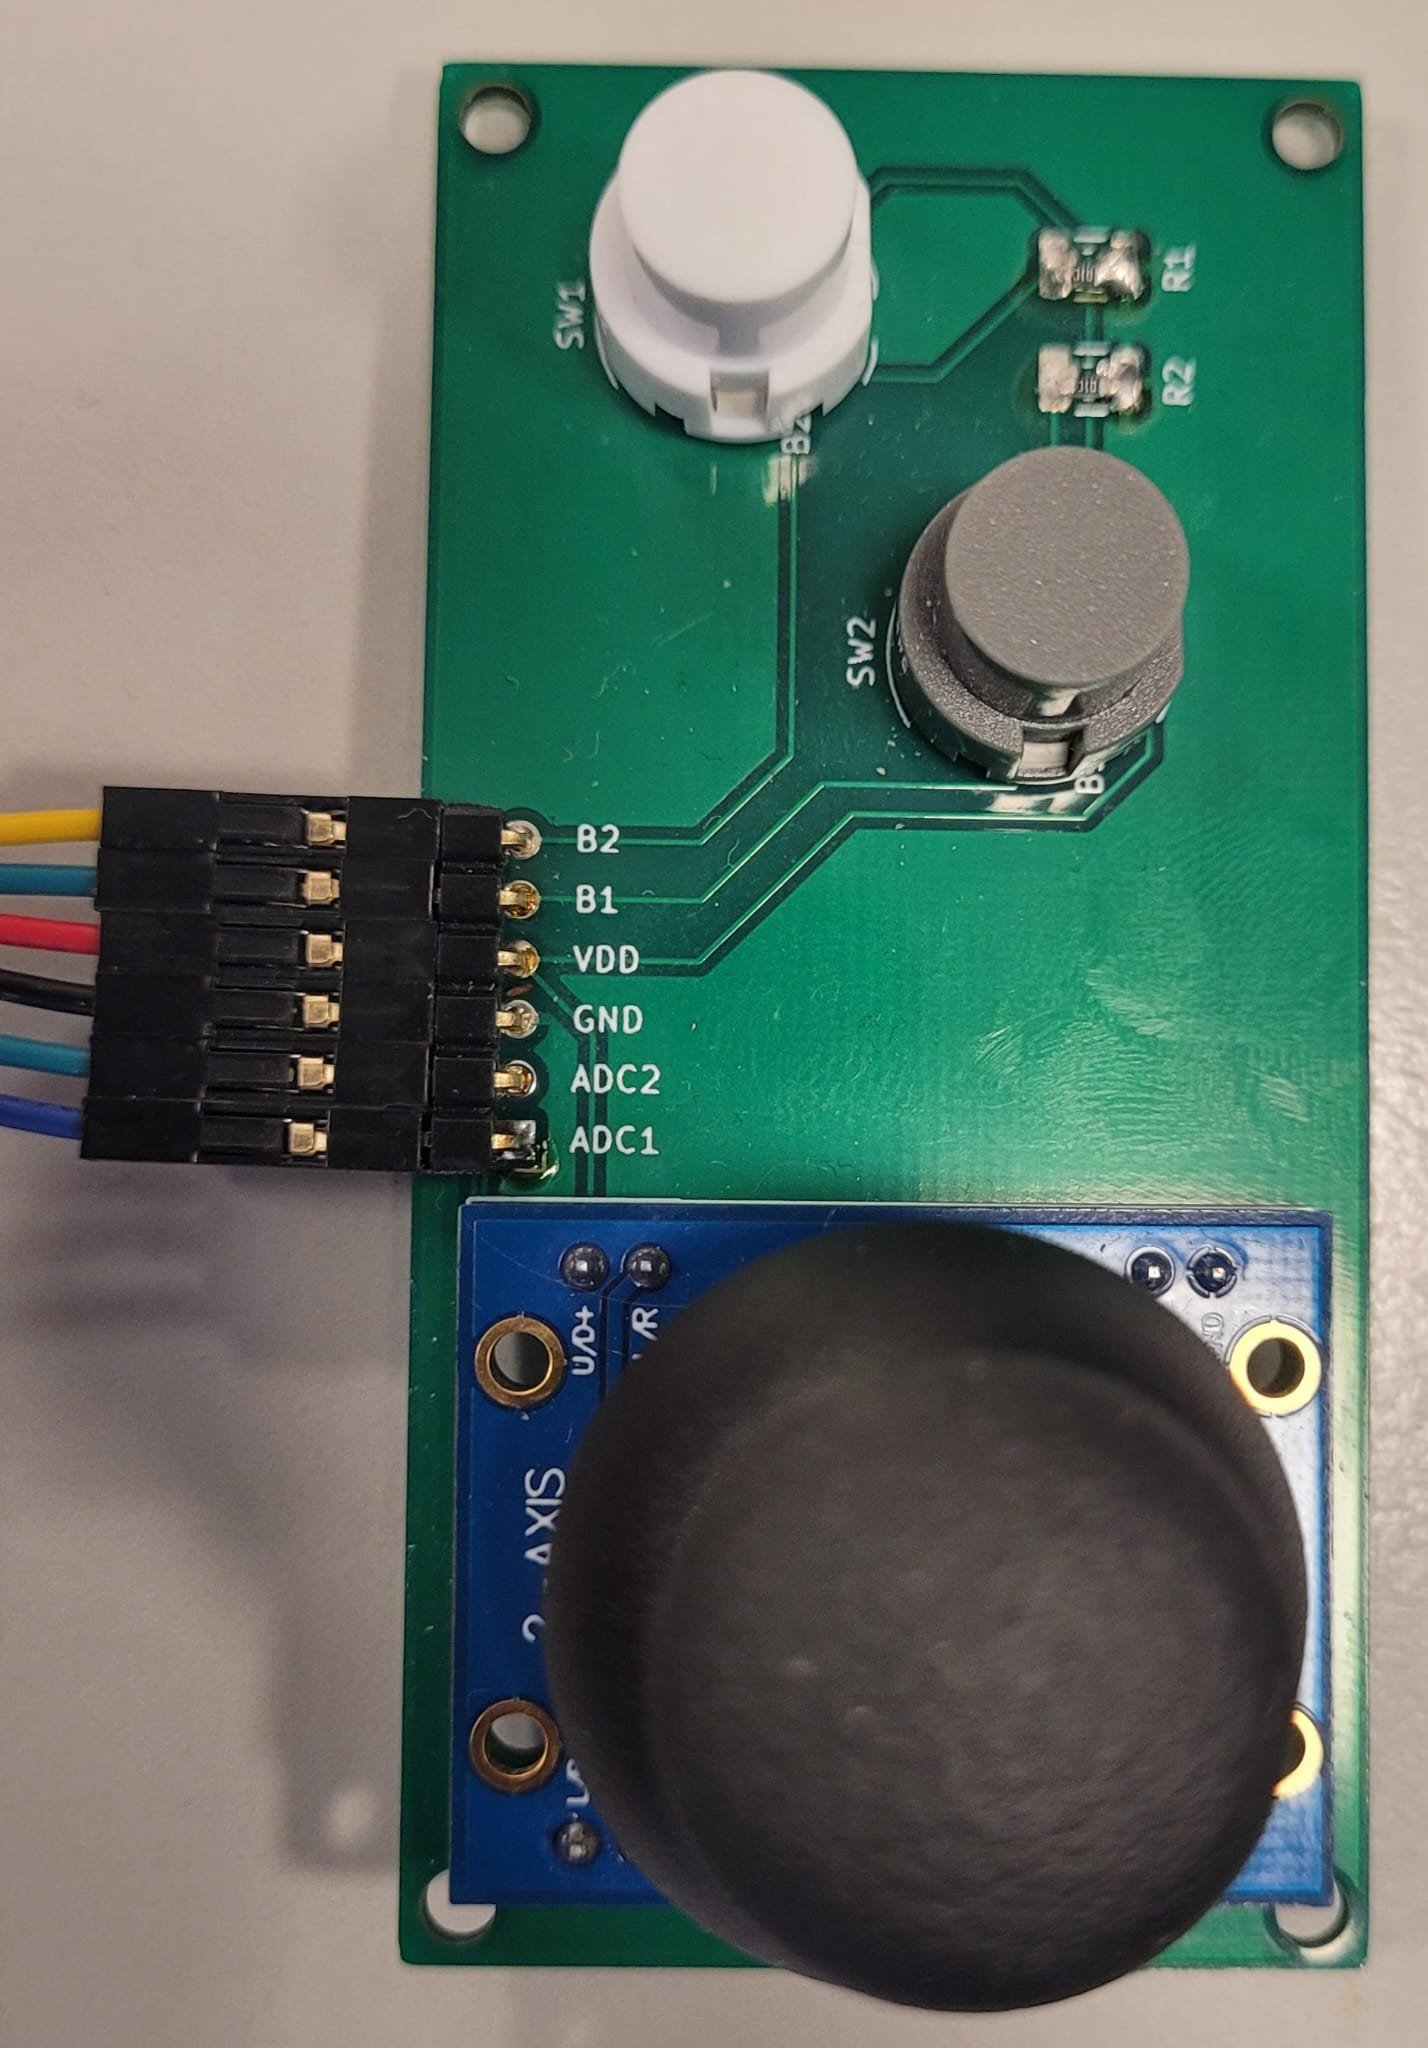
\includegraphics[width=\textwidth]{Picturs/Opsetning/30010joy.jpeg}
        \caption{Billede af 30010-Joystick}
        \label{fig:30010}
    \end{minipage}
    \hspace{0.02\textwidth}
    \begin{minipage}{0.40\textwidth}
        \centering
        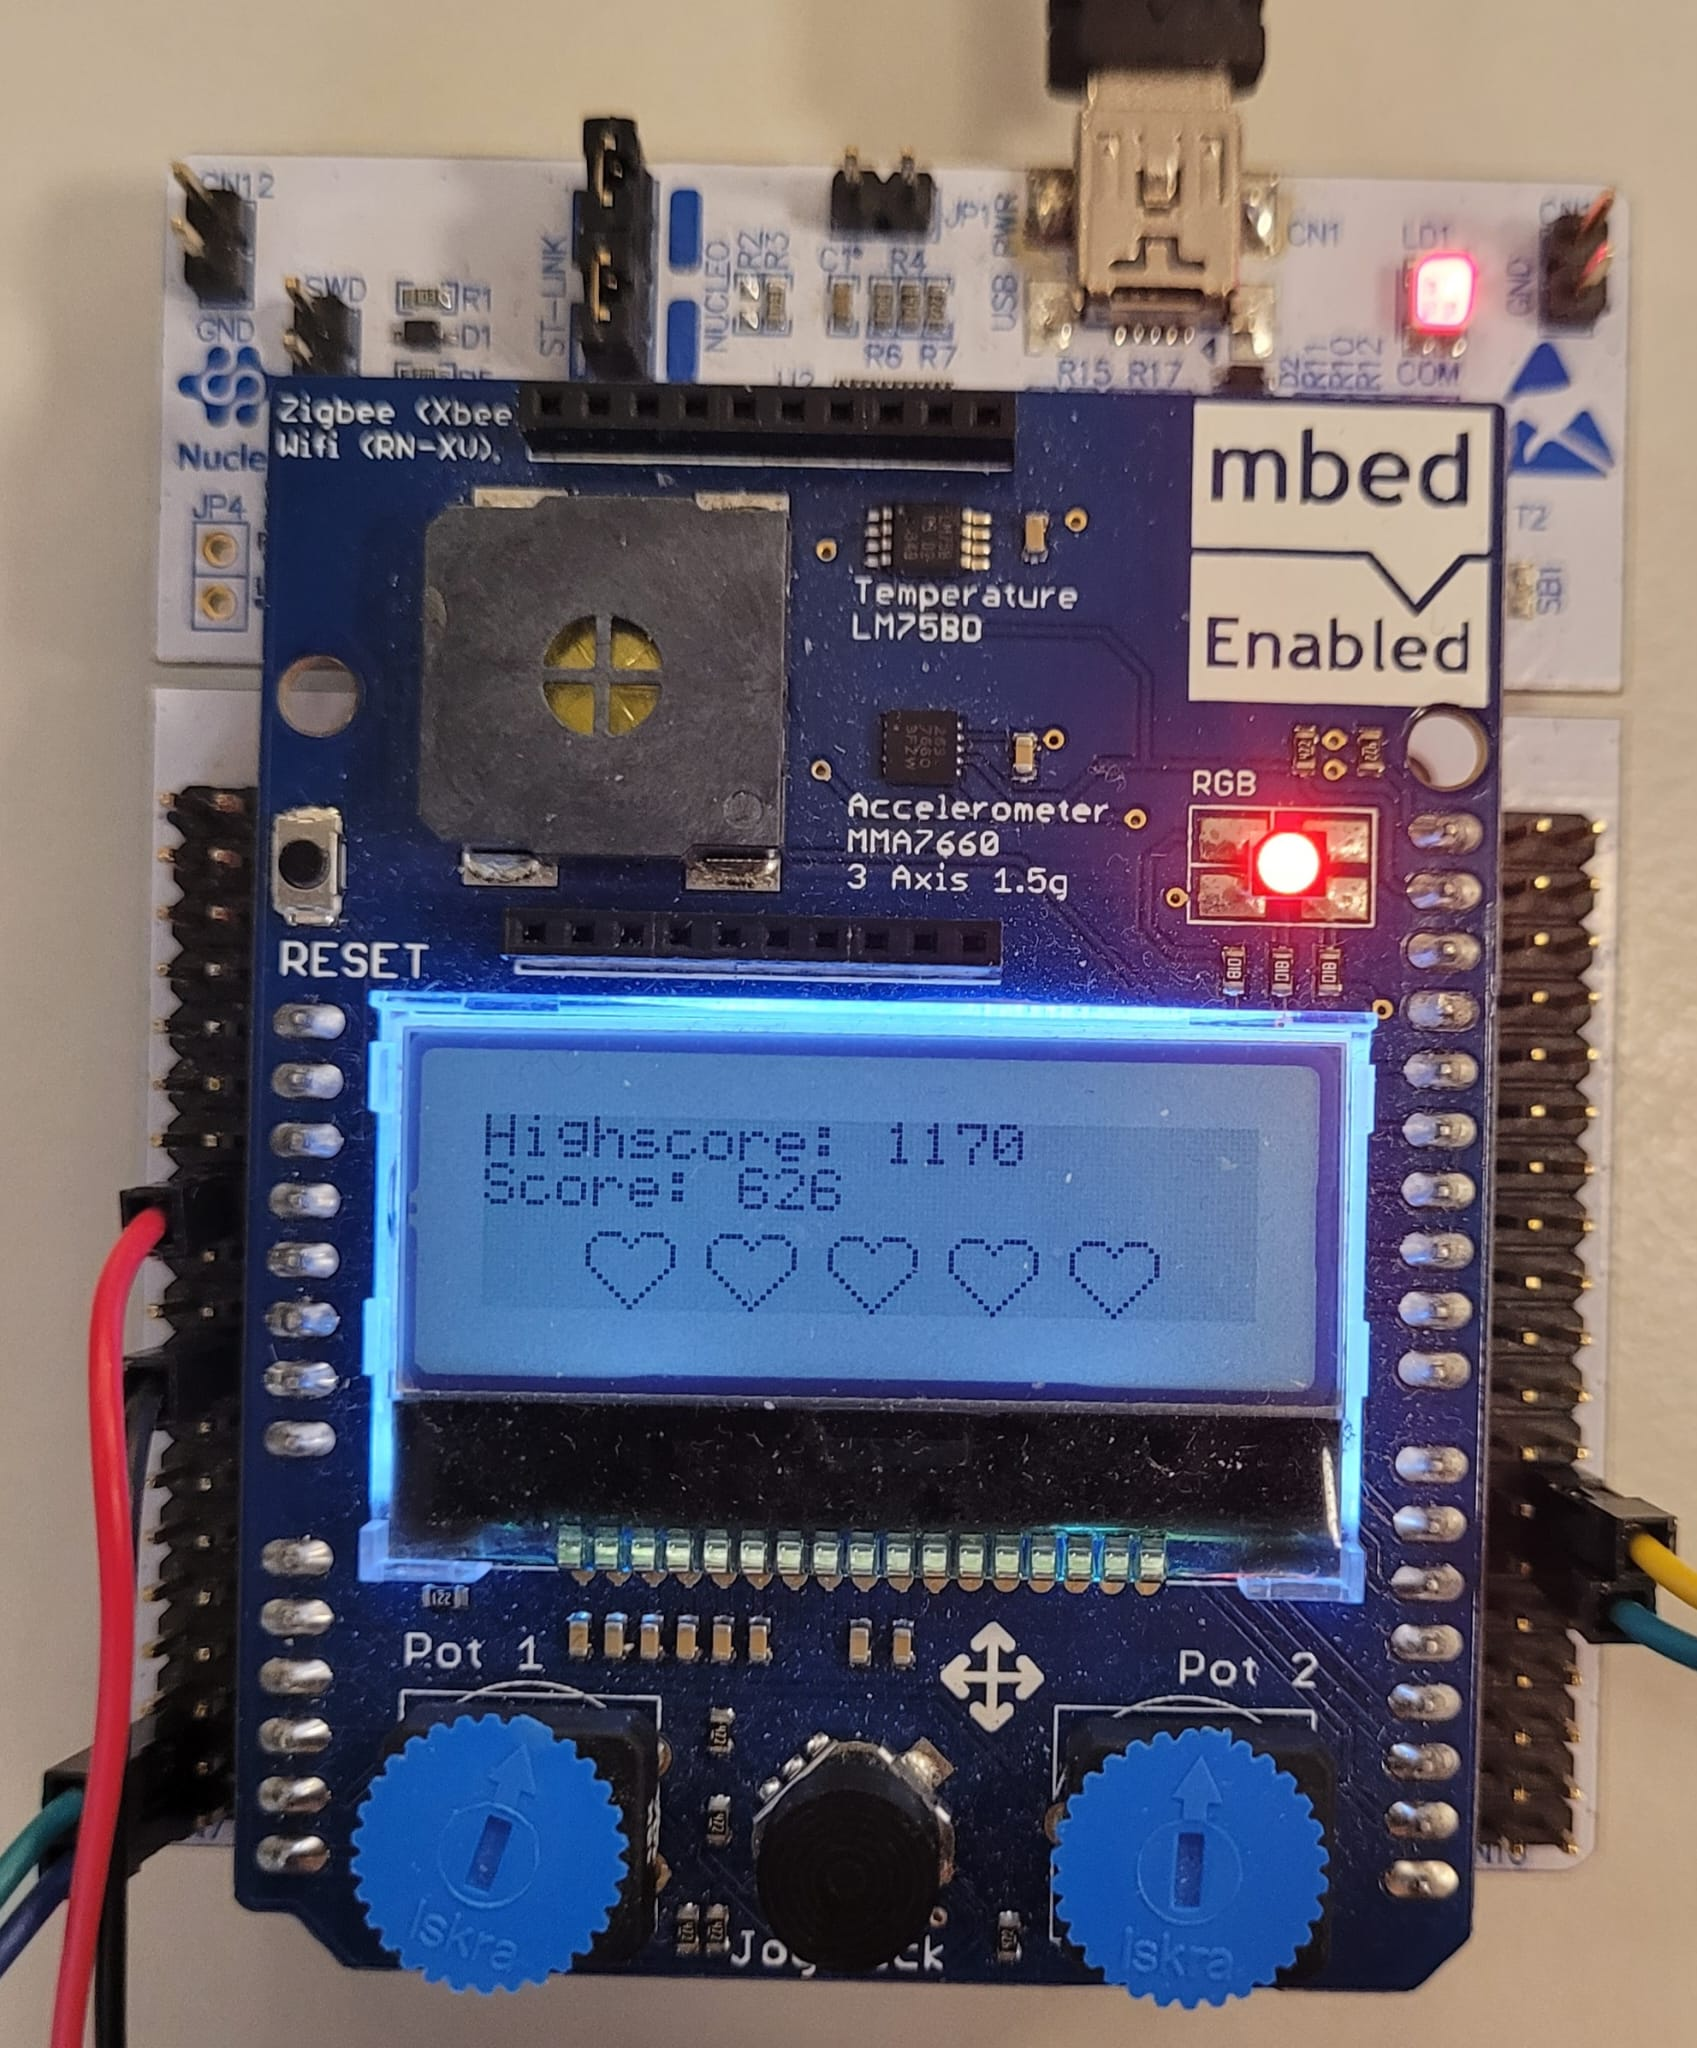
\includegraphics[width=\textwidth]{Picturs/Opsetning/Nucleo.jpeg}
        \caption{Billede af NUCLEO board}
        \label{fig:NUCLEO}
    \end{minipage}
\end{figure}
\vspace{-1em}

For at kunne køre vores program kræver det som sagt en korrekt sammenkobling af hardwaren. Systemet er centreret omkring NUCLEO-F302R8 mikrokontrolleren, hvorpå der er monteret et MBED Extension board. Det eksterne 30010 joystick er essentielt for spillets styring og skal forbindes korrekt til NUCLEO-boardet for at sikre at de analoge og digitale signaler modtages korrekt. Joysticket forbindes til porte på NUCLEO-boardet som følgende angivet (Hardware konfigurationen kan ses på figur \ref{fig:hardware_konfiguration} på næste side): 

\vspace{2em}
\textbf{Strømforsyning:} For aktivere joysticket forbindes VDD på joysticket til 3.3V på NUCLEO boardet, men GND forbindes til Ground.

\vspace{-0.5em}
\textbf{Analog akser (ADC):} ADC1 forbindes til port PC\_3, og ADC2 forbindes til PC\_2. 

\vspace{-0.5em}
\textbf{Digitale knapper:} B1 og B2 forbindes til henholdsvis PA\_6 og PA\_7.

\begin{figure}[H]
    \centering
    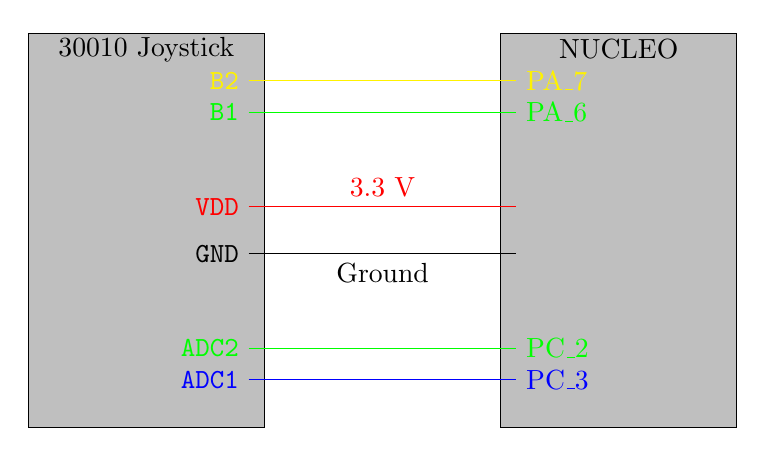
\begin{tikzpicture}
  \draw[fill=lightgray] (0,0) rectangle (3,5);
  \draw[fill=lightgray] (6,0) rectangle (9,5);
  \draw[color=blue] (2.8,0.6) node[left] {\texttt{ADC1}} -- (6.2,0.6) node[right] {PC\_3};
  \draw[color =green] (2.8,1) node[left]{\texttt{ADC2}} -- (6.2,1) node[right] {PC\_2};
  \draw[color=black] (2.8,2.2) node[left] {\texttt{GND}} -- node[below] {Ground} (6.2,2.2);
  \draw[color=red] (2.8,2.8) node[left] {\texttt{VDD}} -- node[above]{3.3 V} (6.2,2.8);
  \draw[color=green] (2.8,4) node[left] {\texttt{B1}} -- (6.2,4) node[right] {PA\_6};
  \draw[color=yellow] (2.8,4.4) node[left] {\texttt{B2}} -- (6.2,4.4) node[right] {PA\_7};
  \node at (7.5,4.8) {NUCLEO};
  \node at (1.5,4.8) {30010 Joystick};
\end{tikzpicture}
    \caption{Hardware konfiguration}
\label{fig:hardware_konfiguration}
\end{figure}
\vspace{-1em}

Joystikets pins kan aflæses på selve 30010 Joysticket, som vis på billede \ref{fig:30010}. De tilsvarende pins på NUCLEO-F302R8 mikrokontrolleren kan aflæses fra STM32F302x8\_NUCLEO\_F302R8\_Pinout pin diagrammet, som kan ses i Appendix \ref{chap:appendiks_1}.

\section{Putty-indstillinger}
\vspace{0.5em}

For at spillet kører smooth og efter hensigten, skal PUTTY terminalen indstilles efter disse bekrivelser.
\begin{itemize}
    \setlength{\itemsep}{4pt}
    \setlength{\parskip}{0pt}
    \setlength{\parsep}{0pt}
    \item Session \rightarrow Serial line: <din serial forbindelse> 
    \item Connnection type: Serial
    \item Speed: 950000
    \item Window \rightarrow set size of window \rightarrow Columns: 100, Rows: 32
    \item Window \rightarrow Translation \rightarrow Remote character set: CP850 
\end{itemize}

\section{Kør Spillet} 
\label{chap:Brugermanual_sec:software}
\vspace{0.5em}

Nu kan spillet køres på mikrocrontrolleren. 
\begin{itemize}
    \setlength{\itemsep}{4pt}
    \setlength{\parskip}{0pt}
    \setlength{\parsep}{0pt}
    \item Download spillet enten via zip på learn eller på \href{https://github.com/wrl6765/DTU-30010-Gruppe-13}{GitHub}
    \item Åben main.c inden i STM32Cube IDE eller din yndlings mikrocontroller konfigurerings app.
    \item sæt configure til AUTO
    \item åben PUTTY med indstillinger fra tidligere sektion og kør koden
\end{itemize}

Sådan! Så brude spillet gerne være sat i gang. Der opfordres til at prøve alle menuer og powerups, samt at forsøge at få en highscore over 1000, så man får den fulde oplevelse.
 
\clearpage 

\chapter{Proces} \label{chap:proces}

For at sikre en struktureret udvikling af spillet, har vi udarbejdet efter en proces, der kombinere indledende planlægning med en initiativ og praktisk tilgang til kodning. Processen kan opdeles i kravspecifikation, systemdesign, implementering og integration. 

\textbf{Idegenerering og kravspecifikation}
\\Projekt forløbet startede ud med en grundig brainstorm-fase. Formålet var her først at definere de absolutte minimumskrav for at opfylde opgaveformuleringen. De den basale ramme var sat på plads, udvidede vi visionen for vores spil og opsatte egen krav til spillets funktionalitet. Denne tidlige fase var afgørende for at sikre at alle gruppemedlemmer havde en fælles forståelse for spillets mekanik, før kodnings processen gik i gang. 

\textbf{Systemarkitektur og opgave fordeling}
\\Inden selve programmeringsfasen påbegyndte, fastlage vi spillets overordnede struktur. Vi valgte en modulær opbygning, hvor koden blev opdelt i parrede .c- og .h-filer. Arkitekturen blev inddelt i fire hovedområder:

\vspace{-5pt}
\begin{itemize}
    \setlength{\itemsep}{0pt}
    \setlength{\parskip}{1pt}
    \setlength{\parsep}{0pt}
    \item Hardware: interaktion med joystick, LED og skærm
    \item Software infrastruktur: Underliggende systemer og kommunikationsproces
    \item Spille logik: beregning af fysik, kollision og bevægelses mønstre
    \item Spille design: visuel præsentation (ASCII-art) og menustruktur
\end{itemize}
\vspace{-5pt}

Opgaven blev fordelt ud fra gruppemedlemmernes individuelle styrker og interesser, hvilket sikrede at alle havde ejerskab over deres spesifike moduler. 

\textbf{Versionsstyring og værktøjer}
\\For at styrke effektiviteten har vi benyttet en række digitale værktøjer: 

\vspace{-5pt}
\begin{itemize}
    \setlength{\itemsep}{0pt}
    \setlength{\parskip}{1pt}
    \setlength{\parsep}{0pt}
    \item GitHub \& VS Code: Vi benyttede GitHub integreret direkte i VS Code. Dette gjorde det muligt løbende at "pushe" og "pulle" kode, hvilket minimerede risikoen for kodekonflikter og gjorde det nemt at gå tibage hvis en ny funktion introducerede fejl.
    \item ST-Link \& Putty: Debugging forgik via en serial forbindelse til Putty, som var med til at give mulighed for at monitorere variabler og programmets tilstand i real tid.
    \item Dokumentation: Rapportskrivning og journal føring skete løbende over Overleaf, mens overblikket over tidsplanen blev styret via et Gantt kort i Excel. 
\end{itemize}

\textbf{Integration og Debugging}
Projektforløbet var opdelt i to faser. Den første uge fungerede som en læring og forberedelsesfase, hvor fokus lå på at lære programmeringssproget C gennem en række undervisningsopgaver \ref{Journal}. Disse opgaver var nødvendige fundamentblokke til vores spil, herunder hardware interaktion, kontrol struktur, og forståelse af data typer.\\
I den anden uge skiftede vi fokus til selve projektet. Da vi allerede havde et godt fundament fra første uges opgaver, kunne vi hurtigt påbegynde integrationsfasen, hvor de isolerede kodebidder og logiske funktioner skulle samles til et sammenhængende spil. Dette var projektets mest kritiske fase, da vi her skulle sikre os at de forskellige moduler spillede sammen i realtid.
Vi lagde stor vægt på at definere klare input og output for vores funktioner således at de passede sammen på tværs af moduler. På trods af forsøget på en grundig planlægning opstod der udfordringer undervej, især omkring synkroniseringen af værdiger mellem forskellige logiske lag. 

\textbf{Kommunikation}
Det sociale og kommunikative fundament har været essentielt for at kunne gennemføre projekt inde for tidsgrænsen. Vi mødte op fysisk på skolen hver dag, hvilket gjorde det muligt at træffe hurtige valg og enriger ved problemer. Ved siden af det fysiske fremmøde havde vi også direkte adgang til alle gruppemedlemmer gennem beskeder, som blev brugt til hurtig opdatering og koordinering unden for skole tid. 

Denne strukturerede tilgang, hvor vi først byggede et solidt fundament i uge 1 og derefter arbejdede intensivt med integration i de følgende 2 uger, har gjort det muligt for os at gå fra de første øvelsesopgaver til et fuldt funktionelt spil med høj teknisk kompleksitet og tilhørende dokumentation.

For at visualisere denne udviklingsproces er der blevet udarbejdet et Gantt diagrammer. Det første diagram herunder \ref{fig:gantt_1}, illustrere vores oprindelige forventning til projektets gang. Det andet diagram \ref{fig:gantt_2} viser det faktiske forløb. Sammenligningen af disse to giver et klart billede af vores evne til at tilpasse os projektets reelle udfordringer undervejs.

\begin{figure}[H]
    \centering
    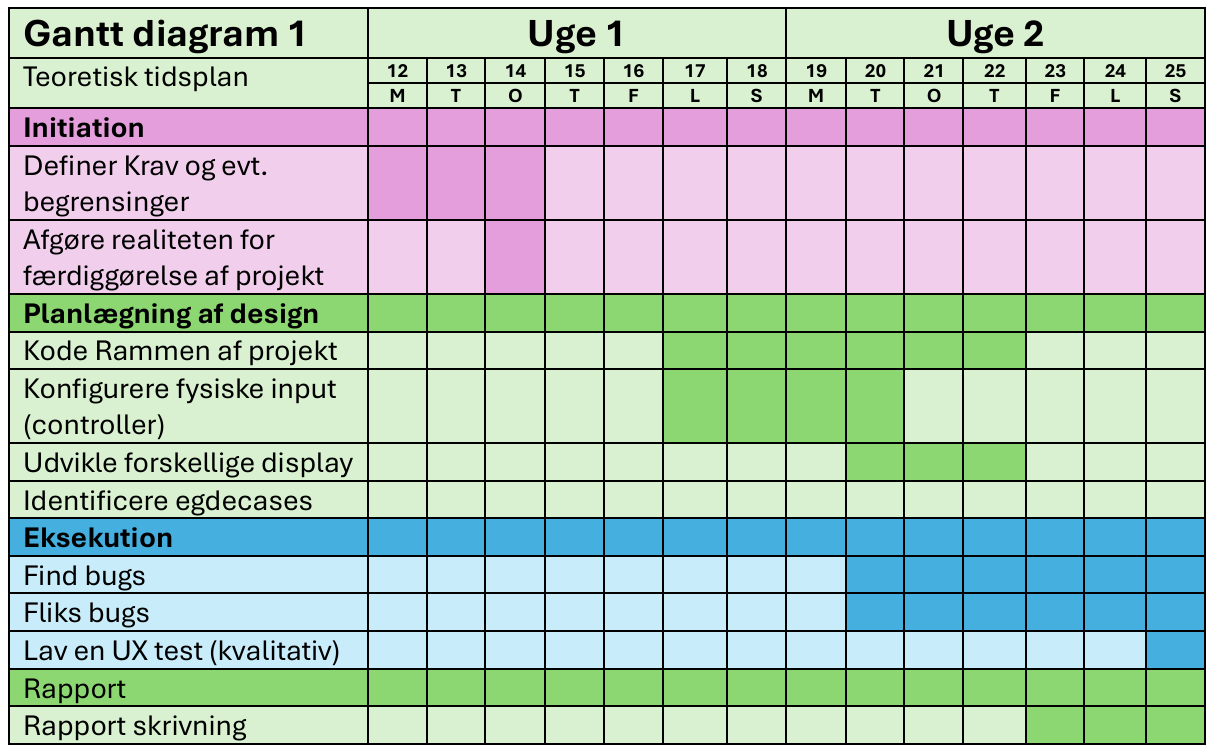
\includegraphics[width=0.81\textwidth]{Picturs/Diagrammer/Gantt1.png}
    \caption{Planlagt tidsplan udarbejdet ved projektstart}
    \label{fig:gantt_1}
\end{figure}
\vspace{-2em}
\begin{figure}[H]
    \centering
    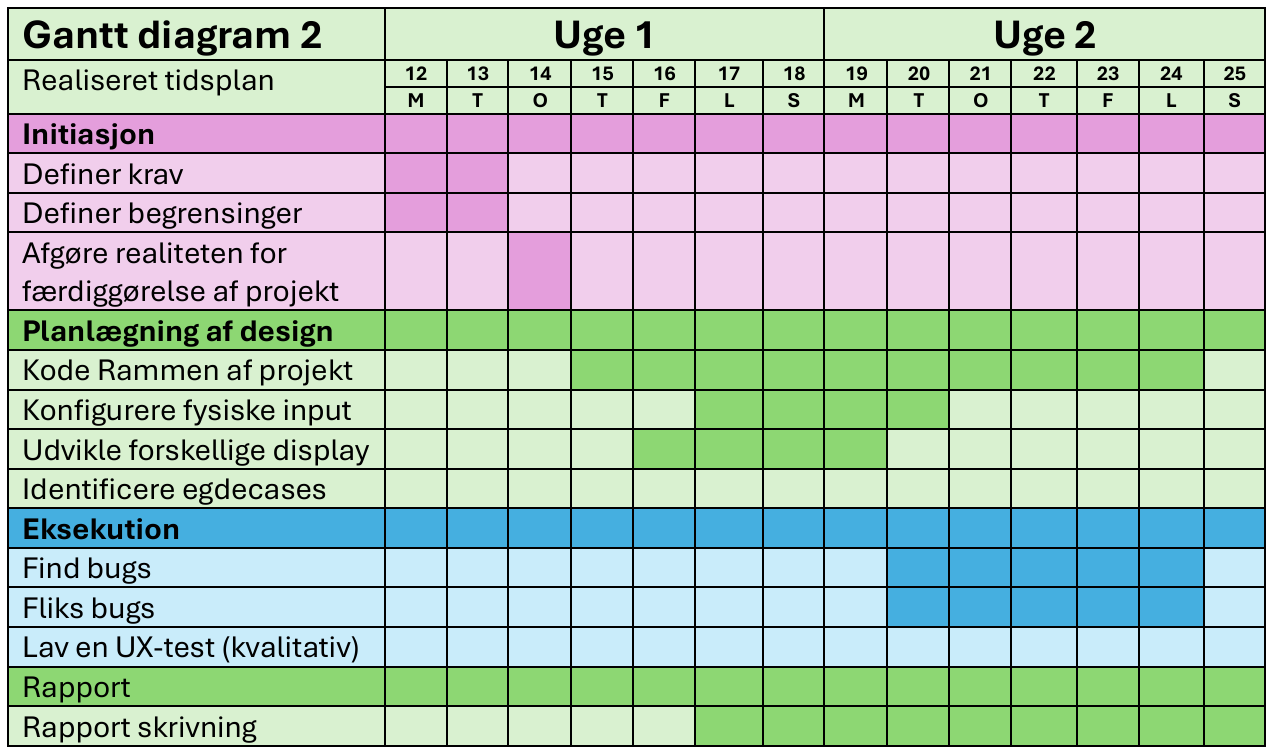
\includegraphics[width=0.81\textwidth]{Picturs/Diagrammer/Gantt2.png}
    \caption{Faktisk tidsforløb og eksekvering af projektfaser}
    \label{fig:gantt_2}
\end{figure} 
\clearpage 

\chapter{Projektverifikation}
For at bekræfte programmeringsprojektet er der behov for systematisk testning af programmet. Dette gøres gennem en række af tests med fokus på både udviklingsprocessen og det færdige produkt. 
Testningen har til formål at sikre, at programmet fungerer som forventet, det er brugervenligt og lever op til de opstillede krav.
Der vil her beskrives hvordan test af udvikling har kørt under udviklingen af projektet, men fokus vil her ligge på test af produktet. 

\section{Test af udvikling}
\vspace{0.5em}
Test af udvikling foregår løbende gennem hele projektets udviklingsfase. Her testes de enkelte funktioner og elementer og dele af programmet, efterhånden som de programmeres og implementeres. Formålet er at kunne identificere fejl eller mangler, så det kan rettes, inden de påvirker resten af programmet.

En vigtig del af udviklingsprocessen er at have gentagne iterationer med fokus på user experience design (UX design). Her afprøver brugere programmet og spillet, og deres interaktioner observeres. Feedback fra disse tests bruges til at forbedre funktionaliteten og designet af spillet. Denne proces gentages flere gange. Dette reducerer risikoen for støre fejl i projektet.

Den generelle struktur af programmet er således at forskellige funktioner og structs er opdelt i forskellige filer i projektet. Dette sikrer at når programmet køres, vil det fremstå præcis hvilke linjer i filer og hermed funktioner som resulterer i et problem, og problemerne med funktionerne kan isoleres, imens de resterende funktioner bevares som er. Dette gør fejlfinding mere overskuelig.

Et konkret eksempel på et problem, der blev identificeret under udviklingstesten, var implementeringen af 30010 joystick-funktionalitet. Den oprindelige idé var, at 30010 joysticket (det store joystick) skulle anvendes til at navigere i menuerne, mens SW1-knappen på 30010 joystick-boardet skulle bruges til at styre spilleren i selve spillet. Under test viste denne løsning sig dog at være problematisk og uhensigtsmæssig, hvilket påvirkede brugeroplevelsen negativt. Gennem gentagende tests og gentagelser blev det derfor besluttet at ændre styresystemets opbygning.

\section{Test af produkt}
\vspace{0.5em}
I forbindelse med test af det færdige produkt var der begrænset tid til at gennemføre omfattende brugertests. Dette betød, at antallet af testpersoner og gentagelser af tests var færre end oprindeligt ønsket, grundet at tiden blev brugt på at udvikle spillet i stedet. På trods af dette blev der stadig lagt vægt på at identificere de mest kritiske fejl og mangler gennem tests af produktets kernefunktioner.

Hvis der havde været mere tid til rådighed, vil teststrategien have været at køre flere brugerbaserede tests med forskellige typer af brugere. Disse tests kunne have givet mere detaljeret feedback på brugervenlighed, spiloplevelse og eventuelle fejlagtige eller problematiske elementer i programmet. Feedback fra brugertests ville være blevet analyseret og anvendt til løbende forbedringer af dele af programmet gennem gentagne tests.

Eventuelle problemer i funktioner der blev identificeret under testningen håndteres og vurderes ud fra deres alvor i programmet. Kritiske fejl prioriteres og rettes hurtigst og bedst muligt, mens mindre problemer håndteres systematisk. Denne tilgang sikrer en struktureret løsning og løbende forbedring af programmet.

Som en del af produkttesten blev den endelige løsning på 30010 joystick-problematikken vurderet og implementeret. I stedet for at anvende 30010 joysticket til at navigere menuen blev mikrocontrollerens knapper brugt til både navigation i menuen og styring af spilleren under spillet. 30010 joysticket blev i stedet anvendt til at styre start accelerationen af bullets i spillet. Denne løsning resulterede i en mere effektiv styring og gjorde det muligt at implementere et player-versus-player (PVP) format med to spillere, hvor styringen er tydeligt opdelt mellem spillerne.
\clearpage 

\chapter{Diskussion} \label{chap:diskussion}
\begin{tabular}{|p{2.4cm}|p{3.6cm}|p{7.4cm}|}
\hline
\textbf{Kategori} & \textbf{Krav} & \textbf{Diskussion og opfyldelse} \\
\hline

Gameplay &
Asteroids / planets with potential field &
Opfyldt. I stedet for et tiltrækkende potentialefelt er der implementeret en forcefield power-up, som får bullets til at accelerere væk fra spilleren. Dette blev vurderet som en mere naturlig løsning i forhold til spillets design. \\
\hline

Gameplay &
3+ stages docked spaceship &
Opfyldt. Spillet indeholder flere stadier, hvor spillerens figur ændrer størrelse over tid. Sværhedsgraden øges gennem mere avancerede projektiltyper og flere samtidige projektiler. \\
\hline

Gameplay &
3+ bullet types + 5+ shot angles &
Opfyldt. Flere projektiltyper (regulær bullet, cannonball og bouncing bullet) er implementeret med forskellig skade, størrelse og hastighed. Skudretninger genereres tilfældigt inden for et 60 graders interval. \\
\hline

Gameplay &
Power-ups &
Opfyldt. Power-ups såsom ekstra liv, score-multiplikator og forcefield spawner hvert tiende sekund og bidrager til variation og strategiske valg. \\
\hline

Gameplay &
Points and lives &
Opfyldt. Spilleren optjener point over tid, og spillet anvender et liv-system, hvor spillet afsluttes, når antallet af liv når nul. \\
\hline

Gameplay &
Random delta-angle &
Opfyldt. Projektilernes skudretning bestemmes ved en randomiseret delta-vinkel, hvilket reducerer forudsigelighed og øger sværhedsgraden. \\
\hline

UI &
Menu, help screen and boss key &
Opfyldt. Spillet indeholder startmenu, hjælpeskærm og boss key, som gør det muligt at pause spillet og returnere til menuen. \\
\hline

UI &
Score / high score display &
Opfyldt. Score og highscore vises både på LCD-displayet og i Putty-terminalen og opdateres løbende. \\
\hline

UI &
RGB LED feedback &
Opfyldt. RGB LED’en giver visuel feedback om spillets tilstand, herunder livstab og aktivt gameplay. \\
\hline

UI &
Partial / full game on LCD &
Opfyldt. LCD-displayet viser score, highscore og antal liv og fungerer som primær visuel feedback. \\
\hline

Controls &
Game controlled by 30010 joystick &
Opfyldt. Spillet styres via 30010-joysticket, som anvendes til både spillerbevægelse og påvirkning af projektiladfærd. \\
\hline

\end{tabular}

 
\clearpage 

\chapter{Konklusion og verifikation} \label{chap:konklusion}


Helt fra starten projektperiode, har vi haft fokus på kommunikation. Det, at vi alle i gruppen viste hvad der forventes af os og hvad der skulle laves, var til en fælles forventningsafstemning for det endelig produkt. Da det overordnede design for spillet skulle bestemmes demokratisk, var det vigtigt for os at vi havde et realistisk syn på hvor langt vi kunne nå på de 2 to uger, samt hvor vores evner og talenter lå, så vi nemmere kunne distribuere arbejdet.
Selvom det til tider var op og ned, kan man se på udfyldelse af krav i Diskussions-afsnittet ovenover, at det gik meget godt. Selve strukturen af koden blev hurtigt sat ind i GitHub, som vi brugte som repository til nemt at dele koden med hinanden. Der er altid stor diskussion for hvad der er den bedste måde at stukturer sin kode og filer på. Nemlig et af de punkter vi kunne have gjort bedre var at definitivt blive enige om hvordan vi vil strukturer koden. Strukturen ændres sig meget, da projektet voksede sig mere omfattede, hvor visse filer var dedikere til kun af holde styr på funktioner. Men set i bakspejlet er disse pointer også noget man lære gennem erfaring; at man ved hvordan man vil strukturer sine filer, inden projektet bliver fyldt med funktioner, der afhænger af hinanden. I Fremtiden er det vigtigt at vi slår fast på vores beslutninger, da omrokeringer i planen, selvom disse kan være nemt forudsigelige, kan hurtigt være med at skabe forvirring, især i større, langvarige projekter, i et programmeringssprog som vi forrige for projektet havde ingen til lav erfaring med. Alt i alt har vi skabt et produkt som overholder kravene fra kursets side af, samt anvendt teknikker fra forelæsninger, øvelser og opgaver, som kulminere til en værktøjskasse af fremgangsmetoder, som langsigtet kan bruges igen.
 
\clearpage 

% %  ======================================================
% % % BIBLIOGRAPHY
% %  ======================================================

\printbibliography[heading=bibintoc,title={Referencer}]
\clearpage 

% %  ======================================================
% % % BACKMATTER
% %  ======================================================

\appendix
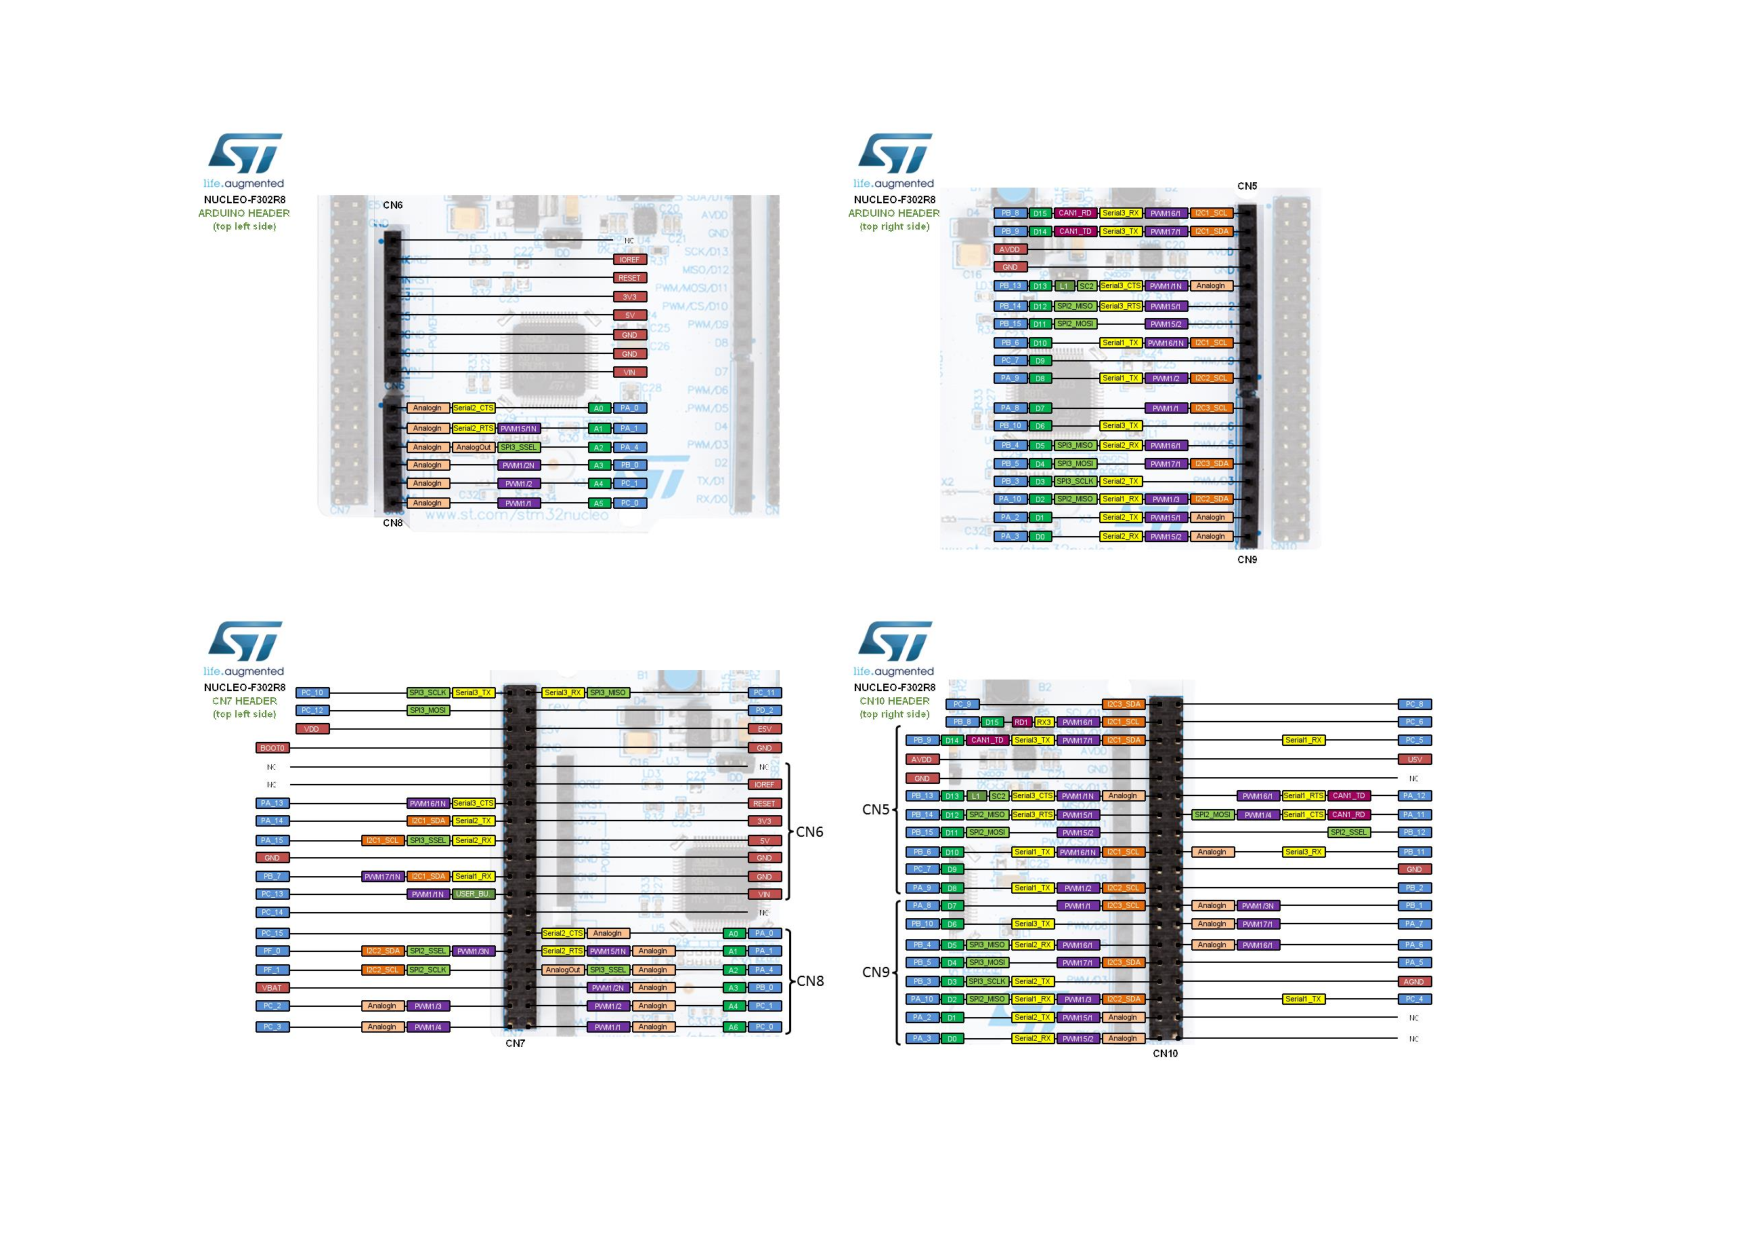
\includepdf[
    pages=1,
    scale=0.9,
    pagecommand={
        \chapter*{Appendiks 1}\label{chap:appendiks_1}
        \addcontentsline{toc}{chapter}{Appendiks 1}
        \vspace{1em}
    }
]{Picturs/Opsetning/STM32F302x8_NUCLEO_F302R8_Pinout (4).pdf}

\clearpage
\chapter{Arbejds fordeling}

\begin{table}[h]
\centering
\renewcommand{\arraystretch}{1.5}
\begin{tabular}{|l|l|c|}
\hline
\multicolumn{3}{|c|}{\textbf{\Large Kodning}} \\ \hline
\textbf{Overordnet kode} & & \textbf{Hvem der har lavet det} \\ \hline

\multirow{4}{*}{Screens}
 & Home screen (design) & William \\ \cline{2-3}
 & Brugermanual (design) & Nikolaj \\ \cline{2-3}
 & Game over screen (design) & Nikolaj \\ \cline{2-3}
 & Implementering af screens &  Nikolaj/William/Daniel \\ \hline

\multirow{4}{*}{Power ups}
 & Health (design/fysik) & Nikolaj/Daniel \\ \cline{2-3}
 & Immunitet (design/fysik) & Nikolaj/Daniel \\ \cline{2-3}
 & Multiplier (design/fysik) & Nikolaj/Daniel \\ \cline{2-3}
 & Implementering af power ups & William/Daniel \\ \hline

\multirow{6}{*}{Hardware}
 & LED & Daniel \\ \cline{2-3}
 & 5 way joystick & Daniel \\ \cline{2-3}
 & 30010 joystick & Safija/Daniel/William \\ \cline{2-3}
 & LCD & Safija \\ \cline{2-3}
 & Timer & Daniel \\ \cline{2-3}
 & Implementering af hardware & William/Daniel \\ \hline

\multirow{4}{*}{Game physics}
 & Player movement &  Nikolaj/Daniel \\ \cline{2-3}
 & Bullet movement &  William/Daniel \\ \cline{2-3}
 & Collision detection & Daniel \\ \cline{2-3}
 & Implementering af game physics &  Daniel \\ \hline

\end{tabular}
\end{table}


\clearpage
\noindent
\centering
\renewcommand{\arraystretch}{1.5}

\begin{tabular}{|l|l|c|}
\hline
\multicolumn{3}{|c|}{\textbf{\Large Rapport}} \\ \hline
\textbf{Overordnet kapitler} & & \textbf{Hvem der har lavet det} \\ \hline

Abstract &  & Safija \\ \hline
Resume &  & Safija \\ \hline
Indledning &  &  Nikolaj \\ \hline

\multirow{6}{*}{Produktudvikling}
 & Undervisningskrav & Safija \\ \cline{2-3}
 & Kravspecifikationer & Safija \\ \cline{2-3}
 & Aim of the game & Safija \\ \cline{2-3}
 & Block Diagram & Safija \\ \cline{2-3}
 & Software arkitektur & Safija \\ \cline{2-3}
 & Flow Chart & Safija \\ \hline

\multirow{4}{*}{Projekt struktur}
 & HAL & William \\ \cline{2-3}
 & AL & William \\ \cline{2-3}
 & Prioriterede funktioner & William/Nikolaj \\ \cline{2-3}
 & Structs & William/Nikolaj \\ \hline

\multirow{3}{*}{Bruger manual}
 & Hardware konfiguration & Safija \\ \cline{2-3}
 & Putty indstillinger & William \\ \cline{2-3}
 & Kør spillet & William \\ \hline

Proces &  & Safija \\ \hline
Test af produkt &  & Nikolaj \\ \hline
Diskussion &  & Daniel \\ \hline
Konklusion &  & William \\ \hline

\end{tabular}

\clearpage
\chapter{Journal}\label{Journal}

\section*{Dag 1\&2. 05-01-2026/06-01-202}
\vspace{1em}

Idag har vi lavet opgave 1,2 \& 3.


\textbf{Exercise 1.1 - Getting Started with the STM32}

STM Cube Ide blev downloaded og configureret. :)

\textbf{Exercise 1.2 - Uploading Code to the STM3}

\begin{figure}[h]
    \centering
    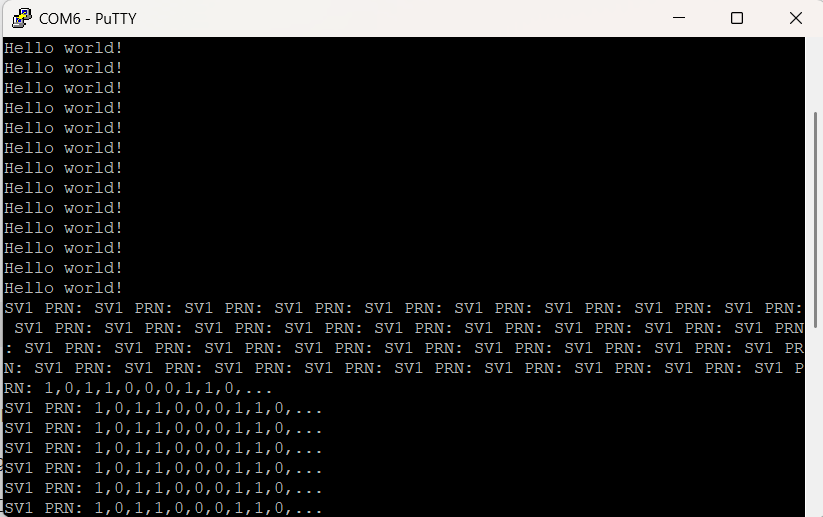
\includegraphics[width=0.75\textwidth]{Picturs/Journal/output 05-01-2026 mikrokontroller.png}
    \caption{Hello world program}
    \vspace{-2em}
\end{figure}

\vspace{1em}

\textbf{Exercise 1.3 Multiple Source Files}

\begin{figure}[h]
    \centering
    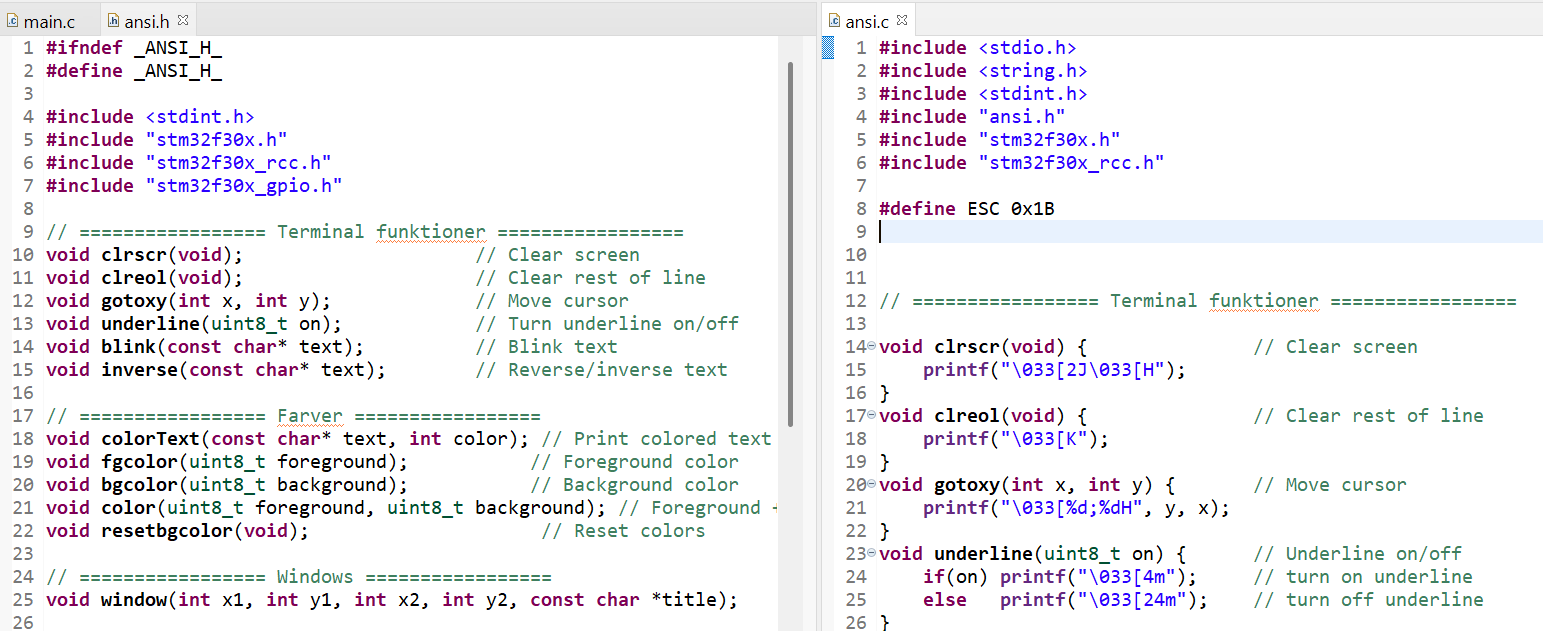
\includegraphics[width=1\textwidth]{Picturs/Journal/opgave1.3.png}
    \caption{ansi.c og ansi.h fil med funktioner}
    \vspace{-2em}
\end{figure}

\vspace{1em}

\textbf{Exercise 1.3 – Debugging}

Vejlednigen for debugging er blevet fuldt.

\vspace{1em}

\textbf{Exercise 1.4 - Integer Number Representation}

\vspace{-1em}

\begin{table}[h]
\centering
\begin{tabularx}{\textwidth}{|l|c|*{5}{>{\centering\arraybackslash}X|}}
\hline
     & Bits & Unsigned & Signed-magnitude & Ones complement & Twos complement & Biased \\ \hline
56   & 8    & 00111000 & 00111000 & 00111000 & 00111000 & 10110111 \\ \hline
178  & 16   & 00000000 10110010 & 00000000 10110010 & 00000000 10011101 & 00000000 10011110 & 10000000 10110001 \\ \hline
1002 & 16   & 00000011 11101010 & 00011101 10100010 & 00000011 11101010 & 00000011 11101010 & 10000011 11101001 \\ \hline
7586 & 16   & 00011101 10100010 & 00011101 10100010 & 00011101 10100010 & 00011101 10100010 & 10011101 10100001 \\ \hline
\end{tabularx}
\end{table}

\vspace{-2em}

\begin{table}[h]
\centering
\begin{tabularx}{\textwidth}{|l|c|*{5}{>{\centering\arraybackslash}X|}}
\hline
     & Bits & Unsigned & Signed-magnitude & Ones complement & Twos complement & Biased \\ \hline
-56  & 8    & ---      & 10111000         & 11000111        & 11001000        & 10110111 \\ \hline
-178 & 16   & ---      & 10000000 10110010 & 11111110 1001101 & 11111110 1001110 & --- \\ \hline
-1002& 16   & ---      & 10011101 10100010 & 11100010 01011101 & 11100010 01011110 & --- \\ \hline
-7586& 16   & ---      & 10011101 10100010 & 11100010 01011101 & 11100010 01011110 & --- \\ \hline
\end{tabularx}
\end{table}

\begin{lstlisting}
x = 1
y = not 0

if x==y:
    print("same")
else:
    print("Not same")
\end{lstlisting}

\vspace{-2em}

\textbf{Exercise 2.1 - ANSI Escape Codes}

\begin{lstlisting}
#ifndef ANSI_H_
#define ANSI_H_

#include <stdint.h>
#include <stdio.h>

void fgcolor(uint8_t foreground);
void bgcolor(uint8_t background);
void color(uint8_t foreground, uint8_t background);

#endif /* ANSI_H_ */
\end{lstlisting}

\vspace{-2em}

\textbf{Exercise 2.2 - Drawing Windows}
\begin{figure}[h]
    \centering
    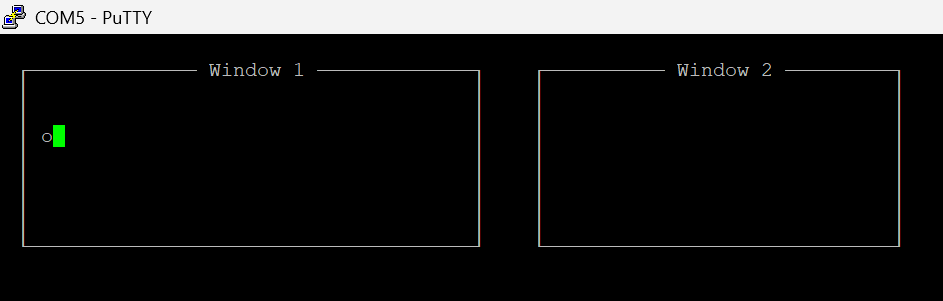
\includegraphics[width=0.82\textwidth]{Picturs/Journal/opgave2.2.png}
    \caption{Windows program}
    \vspace{-2em}
\end{figure}

\textbf{Exercise 2.3 - Bit Manipulation Question}

\keepXColumns
\begin{tabularx}{\textwidth}{|l|X|X|}
\hline
\textbf{ID} & \textbf{Spørgsmål} & \textbf{Svar} \\ \hline
\endhead

0x00 & What is 0x14 in binary? & 1=0001, 4=0100 $\rightarrow$ 14=00010100 \\ \hline
0x01 & What is 0xE6 in binary? & 11100110 \\ \hline
0x02 & What is 0x58 in binary? & 01011000 \\ \hline
0x03 & What is 10110111b in hexadecimal? & 0xB7 \\ \hline
0x04 & What is 10011111b in hexadecimal? & 0x9F \\ \hline
0x05 & What is 00111101b in hexadecimal? & 0x3D \\ \hline
0x06 & How do you turn ON bits 4 and 7 in a byte? & 0x90 (10010000) \\ \hline
0x07 & How do you turn OFF bits 2 and 5 in a byte? & 0x24 (00100100) \\ \hline
0x08 & How do you write -1 in binary, assuming size of a byte? & 10000001 (Signed-mag) / 11111111 (2's comp) \\ \hline
0x09 & How do you write -2 in binary, assuming size of a byte? & 10000010 (Signed-mag) / 11111110 (2's comp) \\ \hline
0x0A & What is 00001000b in decimal, assuming unsigned notation? & 8 \\ \hline
0x0B & What is 00001000b in decimal, assuming signed notation? & 8 \\ \hline
0x0C & What is 11111110b in decimal, assuming unsigned notation? & 254 \\ \hline
0x0D & What is 11111110b in decimal, assuming signed notation? & -2 (2's complement) \\ \hline
0x0E & What is the highest value you can store in a signed byte? & 127 (01111111) \\ \hline
0x0F & What is the highest value you can store in an unsigned byte? & 255 (11111111) \\ \hline
0x10 & What is the lowest value you can store in a signed byte? & -128 (10000000 i 2's comp) \\ \hline
0x11 & What is the lowest value you can store in an unsigned byte? & 0 (00000000) \\ \hline
0x12 & How do you tell if a signed byte is positive or negative? & Most left bit; 1 $\rightarrow$ neg, 0 $\rightarrow$ pos \\ \hline
0x13 & How do you change the sign of a binary number? & Invertér alle bits og læg 1 til (2's comp) \\ \hline
0x14 & How do you multiply a binary number by two? & Forskyd alle tal én gang til venstre ($<< 1$) \\ \hline
0x15 & How do you divide a binary number by two? & Forskyd tal til højre ($>> 1$) \\ \hline
0x16 & When dividing by two, how is rounding performed? & Ved ulige tal: Rund ned (standard shift) eller rund op ved at tilføje 1 før shift. \\ \hline
0x17 & What is the result of 0x12 | 0x01 in binary and hexadecimal? & 00010011 (0x13) \\ \hline
0x18 & What is the result of 0x13 \& 0xFE in binary and hexadecimal? & 00010010 (0x12) \\ \hline
0x19 & What is the result of $\sim$0x3F in binary and hexadecimal? & 11000000 (0xC0) \\ \hline
0x1A & What is the result of $\sim$0x01 in binary and hexadecimal? & 11111110 (0xFE) \\ \hline
0x1B & What is the result of 0x0C $>>$ 2 in binary and hexadecimal? & 00000011 (0x03) \\ \hline
0x1C & What is the result of 0x0C $>>$ 4 in binary and hexadecimal? & 00000000 (0x00) \\ \hline
0x1D & What is the result of 0x0C $<<$ 4 in binary and hexadecimal? & 11000000 (0xC0) \\ \hline
\end{tabularx}

\textbf{Exercise 3.1 – Creating a Look-up Table}

\begin{lstlisting}
#ifndef FIXED_POINT_H_
#define FIXED_POINT_H_

#include <stdint.h>

const int16_t lut[512];

void printFix(int32_t i);

int16_t sinus(int16_t);
int16_t cosinus(int16_t degree);

#endif
\end{lstlisting}

\vspace{-2em}

Declaring all of the functions and including necesarry librarie(s).

\vspace{1em}

\begin{lstlisting}
#include "fixed_point.h"

const int16_t lut[512] = {
    0, 201, 402, 603, 804, 1005, 1205,
    1406, 1606, 1806, 2005, 2205, 2404, 2603,
    2801, 2999, 3196, 3393, 3590, 3785, 3981,
    4175, 4370, 4563, 4756, 4948, 5139, 5330,
    5519, 5708, 5896, 6083, 6270, 6455, 6639,
    6822, 7005, 7186, 7366, 7545, 7723, 7900,
    8075, 8249, 8423, 8594, 8765, 8934, 9102,
    9268, 9433, 9597, 9759, 9920, 10079, 10237,
    10393, 10548, 10701, 10852, 11002, 11150, 11297,
    11441, 11585, 11726, 11865, 12003, 12139, 12273,
    12405, 12536, 12664, 12791, 12915, 13038, 13159,
    13278, 13394, 13509, 13622, 13733, 13841, 13948,
    14052, 14154, 14255, 14353, 14449, 14542, 14634,
    14723, 14810, 14895, 14977, 15058, 15136, 15212,
    15285, 15356, 15425, 15492, 15556, 15618, 15678,
    15735, 15790, 15842, 15892, 15940, 15985, 16028,
    16068, 16106, 16142, 16175, 16206, 16234, 16260,
    16283, 16304, 16323, 16339, 16352, 16363, 16372,
    16378, 16382, 16383, 16382, 16378, 16372, 16363,
    16352, 16339, 16323, 16304, 16283, 16260, 16234,
    16206, 16175, 16142, 16106, 16068, 16028, 15985,
    15940, 15892, 15842, 15790, 15735, 15678, 15618,
    15556, 15492, 15425, 15356, 15285, 15212, 15136,
    15058, 14977, 14895, 14810, 14723, 14634, 14542,
    14449, 14353, 14255, 14154, 14052, 13948, 13841,
    13733, 13622, 13509, 13394, 13278, 13159, 13038,
    12915, 12791, 12664, 12536, 12405, 12273, 12139,
    12003, 11865, 11726, 11585, 11441, 11297, 11150,
    11002, 10852, 10701, 10548, 10393, 10237, 10079,
    9920, 9759, 9597, 9433, 9268, 9102, 8934,
    8765, 8594, 8423, 8249, 8075, 7900, 7723,
    7545, 7366, 7186, 7005, 6822, 6639, 6455,
    6270, 6083, 5896, 5708, 5519, 5330, 5139,
    4948, 4756, 4563, 4370, 4175, 3981, 3785,
    3590, 3393, 3196, 2999, 2801, 2603, 2404,
    2205, 2005, 1806, 1606, 1406, 1205, 1005,
    804, 603, 402, 201, 0, -201, -402,
    -603, -804, -1005, -1205, -1406, -1606, -1806,
    -2005, -2205, -2404, -2603, -2801, -2999, -3196,
    -3393, -3590, -3785, -3981, -4175, -4370, -4563,
    -4756, -4948, -5139, -5330, -5519, -5708, -5896,
    -6083, -6270, -6455, -6639, -6822, -7005, -7186,
    -7366, -7545, -7723, -7900, -8075, -8249, -8423,
    -8594, -8765, -8934, -9102, -9268, -9433, -9597,
    -9759, -9920, -10079, -10237, -10393, -10548, -10701,
    -10852, -11002, -11150, -11297, -11441, -11585, -11726,
    -11865, -12003, -12139, -12273, -12405, -12536, -12664,
    -12791, -12915, -13038, -13159, -13278, -13394, -13509,
    -13622, -13733, -13841, -13948, -14052, -14154, -14255,
    -14353, -14449, -14542, -14634, -14723, -14810, -14895,
    -14977, -15058, -15136, -15212, -15285, -15356, -15425,
    -15492, -15556, -15618, -15678, -15735, -15790, -15842,
    -15892, -15940, -15985, -16028, -16068, -16106, -16142,
    -16175, -16206, -16234, -16260, -16283, -16304, -16323,
    -16339, -16352, -16363, -16372, -16378, -16382, -16383,
    -16382, -16378, -16372, -16363, -16352, -16339, -16323,
    -16304, -16283, -16260, -16234, -16206, -16175, -16142,
    -16106, -16068, -16028, -15985, -15940, -15892, -15842,
    -15790, -15735, -15678, -15618, -15556, -15492, -15425,
    -15356, -15285, -15212, -15136, -15058, -14977, -14895,
    -14810, -14723, -14634, -14542, -14449, -14353, -14255,
    -14154, -14052, -13948, -13841, -13733, -13622, -13509,
    -13394, -13278, -13159, -13038, -12915, -12791, -12664,
    -12536, -12405, -12273, -12139, -12003, -11865, -11726,
    -11585, -11441, -11297, -11150, -11002, -10852, -10701,
    -10548, -10393, -10237, -10079, -9920, -9759, -9597,
    -9433, -9268, -9102, -8934, -8765, -8594, -8423,
    -8249, -8075, -7900, -7723, -7545, -7366, -7186,
    -7005, -6822, -6639, -6455, -6270, -6083, -5896,
    -5708, -5519, -5330, -5139, -4948, -4756, -4563,
    -4370, -4175, -3981, -3785, -3590, -3393, -3196,
    -2999, -2801, -2603, -2404, -2205, -2005, -1806,
    -1606, -1406, -1205, -1005, -804, -603, -402,
    -201};

void printFix(int32_t i) {
// Prints a signed 16.16 fixed point number
    if ((i & 0x80000000) != 0) { // Handle negative numbers
        printf("-");
        i = ~i + 1;
    }

    printf ("%ld .%04 ld", i >> 16 , 10000 * ( uint32_t )(i & 0 xFFFF ) >> 16) ;
    // Print a maximum of 4 decimal digits to avoid overflow
    }

    int16_t sinus ( int16_t degree ) {
    return lut [ degree %512];
    }

    int16_t cosinus ( int16_t degree ) {
    return lut [( degree +128) %512];
    }
}

\end{lstlisting}

\vspace{-1em}

Pasting in all of the LUT values as well as writing the functions: printFix, sinus, and cosinus.

\vspace{1em}

\begin{lstlisting}
# include " stm32f30x_conf .h" // STM32 config
# include " 30010 _io.h" // Input / output library for this course
# include " ansi .h"
# include " fixed_point .h"

int main ( void ){
    uart_init (9600) ;
    printFix ( sinus (124) << 2) ;
    while (1) {}
}
\end{lstlisting}

\vspace{-2em}

Including all files and returning the result

\textbf{Exercise 3.2 – Sin and Cos Functions}

\begin{lstlisting}
#include <stdio.h>
#include <math.h>
#include <stdint.h>

int rotatevector(double x, double y, double angle,
                 double *diffx, double *diffy) {
    *diffx = x * cos(angle) - y * sin(angle);
    *diffy = x * sin(angle) + y * cos(angle);
    return 0;
}

int main(void) {
    double dangle;
    double a, b;
    double spliffy, spliffx;

    scanf("%lf", &dangle);
    scanf("%lf", &a);
    scanf("%lf", &b);

    rotatevector(a, b, dangle, &spliffx, &spliffy);
    printf("%f, %f\n", spliffx, spliffy);

    return 0;
}
\end{lstlisting}

\textbf{Exercise 3.3 - Vector Rotations}

\textbf{Exercise 3.4 - Bit Manipulation Questions Continued}

\keepXColumns
\begin{tabularx}{\textwidth}{|l|X|X|}
\hline
\textbf{ID} & \textbf{Spørgsmål} & \textbf{Svar} \\ \hline
\endhead
0x1E & How do you convert a char into 8.8 notation? & Shift 8 bits til venstre ($<< 8$) eller gange med 256. \\ \hline
0x1F & How do you convert an 8.8 value into a char? & Shift 8 bits til højre ($>> 8$). \\ \hline
0x20 & What is the smallest, positive, non-zero value you can store? & 1/256 (0.00390625) \\ \hline
0x21 & What happens if you add two 8.8 values? & Læg heltal og decimaler sammen normalt. \\ \hline
0x22 & What happens if you multiply two 8.8 values? & Giver et 16.16 tal, kræver shift $>> 8$ for at vende tilbage til 8.8. \\ \hline
0x23 & What happens if you multiply an 8.8 value with a char? & Resultatet forbliver i 8.8 format. \\ \hline
0x24 & What about rounding when you convert an 8.8 value to a char? & Tilføj 0x80 ($0.5$ i 8.8) før shift $>> 8$. \\ \hline
0x25 & How do you make it round correctly? & $\pm$ 0x80 afhængigt af fortegn. \\ \hline
0x26 & What is the decimal number 0.125 in hexadecimal? & 0.2 \\ \hline
0x27 & What is the decimal number 0.25 in hexadecimal? & 0.4 \\ \hline
0x28 & What is the decimal number 2.125 in hexadecimal? & 2.2 \\ \hline
0x29 & What is the decimal number 2.25 in hexadecimal? & 2.4 \\ \hline
0x2A & What is the result of 0.125*0.25 using fixed point? & 0,03125 \\ \hline
0x2B & What is the result of 2.125*2.25 using fixed point? & 4,78125 \\ \hline
0x2C & What goes wrong in question (0x2B)? & Overflow kan forekomme hvis resultatet overstiger 8.8. \\ \hline
0x2D & How can the issue of (0x2B) be addressed? & Brug en større variabel (f.eks. 16.16) til mellemregningen. \\ \hline
\end{tabularx}

\clearpage
\section*{Dag 3. 07-01-2026}
\vspace{1em}

\textbf{Exercise 4.1 – Graphics / Exercise 4.2 – Collisions}
\vspace{1em}

\begin{lstlisting}
#ifndef __tennisball__
#define __tennisball__

#define gotoxy(x,y) printf("\x1B[%d;%df",y,x)

#endif
\end{lstlisting}
\vspace{-2em}

Start koordinater blev initialized.

\vspace{1em}
\begin{lstlisting}
#include <stdio.h>
#include "escape.h"
#include <unistd.h>
#include <signal.h>

int draw(int x,int y,int w,int h);
void cleanup(int sig);
int animation(int vx,int vy);

int main(){

    printf("\x1B[2J");
    gotoxy(1,1);
    draw(1,1,20,10);
    animation(1,1);
    cleanup(0);

    // for (int i =0;i<256;i++){
    //     printf("%d: %c\n",i,i);
    // }

    return 0;
}

int draw(int x,int y,int w,int h){
    for (int py = y ; py < y+h ; py++){
        for (int px = x ; px < x+w ; px++){
            gotoxy(px, py);
            if ((px == x && py == y) ||
                (px == w && py == y) ||
                (px == w && py == h) ||
                (px == x && py == h)) {
                printf("+");
            }
            else if ((py < y+h && px == x) || (py < y+h && px == w)){
                printf("|");
            }
            else if (px < x+w && py == y){
                printf("-");
            }
            else if (py == h){
                printf("-");
            }
        }
    }
}

void cleanup(int sig) {
    printf("\x1b[?25h");
    printf("\x1b[0m");
    fflush(stdout);
    _exit(0);
}

int animation(int vx,int vy){
    int x = 10;
    int y = 5;
    int oldx = x;
    int oldy = y;
    int n = 0;

    signal(SIGINT, cleanup);

    while (1){

        printf("\x1b[%d;%dH ", oldy, oldx);

        oldx = x;
        oldy = y;

        fflush(stdout);

        x += vx;
        y += vy;

        printf("\x1b[%d;%dH", y, x);
        printf("\x1b[31mO\x1b[0m");

        if (x <= 1 || x >= 20) vx = -vx;
        if (y <= 1 || y >= 10) vy = -vy;

        usleep(30000);

        if (y >= 10){
            printf("\n\n\nnumber of bounces: %d", n++);
        }
    }
}
\end{lstlisting}
\vspace{-2em}

program blev designet og kørt.

\textbf{Exercise 4.3 – Documentation}

Et ok flowchart blev kreeret.
\clearpage
\section*{Dag 4\&5. 08-01-2026/09-01-2026}
\vspace{1em}

\textbf{Exercise 5.1 - Detecting a Joystick Interaction}
\begin{lstlisting}
#include "stm32f30x_conf.h"
#include "30010_io.h"
#include <stdint.h>

// --------------------------------------------------
// Read joystick state
// --------------------------------------------------
uint8_t readJoystick(void)
{
    uint8_t state = 0;

    if (GPIOA->IDR & (1 << 4)) state |= (1 << 0); // UP
    if (GPIOB->IDR & (1 << 0)) state |= (1 << 1); // DOWN
    if (GPIOC->IDR & (1 << 1)) state |= (1 << 2); // LEFT
    if (GPIOC->IDR & (1 << 0)) state |= (1 << 3); // RIGHT
    if (GPIOB->IDR & (1 << 5)) state |= (1 << 4); // CENTER

    return state;
}

// --------------------------------------------------
// Simple delay
// --------------------------------------------------
void delay_ms(uint32_t ms)
{
    for (uint32_t i = 0; i < ms * 8000; i++) {
        __NOP();
    }
}

// --------------------------------------------------
// Main
// --------------------------------------------------
int main(void)
{
    uart_init(9600);

    // Enable GPIO clocks
    RCC->AHBENR |= RCC_AHBPeriph_GPIOA
                | RCC_AHBPeriph_GPIOB
                | RCC_AHBPeriph_GPIOC;

    // Configure joystick pins as INPUT, NO pull-up/down

    // PA4 - UP
    GPIOA->MODER &= ~(0x3 << (4 * 2));
    GPIOA->PUPDR &= ~(0x3 << (4 * 2));

    // PB0 - DOWN
    GPIOB->MODER &= ~(0x3 << (0 * 2));
    GPIOB->PUPDR &= ~(0x3 << (0 * 2));

    // PB5 - CENTER
    GPIOB->MODER &= ~(0x3 << (5 * 2));
    GPIOB->PUPDR &= ~(0x3 << (5 * 2));

    // PC0 - RIGHT
    GPIOC->MODER &= ~(0x3 << (0 * 2));
    GPIOC->PUPDR &= ~(0x3 << (0 * 2));

    // PC1 - LEFT
    GPIOC->MODER &= ~(0x3 << (1 * 2));
    GPIOC->PUPDR &= ~(0x3 << (1 * 2));

    uint8_t lastState = 0;

    while (1)
    {
        uint8_t state = readJoystick();

        if (state != lastState)
        {
            if (state == 0) {
                printf("RELEASED\r\n");
            } else {
                if (state & (1 << 0)) printf("UP\r\n");
                if (state & (1 << 1)) printf("DOWN\r\n");
                if (state & (1 << 2)) printf("LEFT\r\n");
                if (state & (1 << 3)) printf("RIGHT\r\n");
                if (state & (1 << 4)) printf("CENTER\r\n");
            }

            lastState = state;
            delay_ms(200);   // simple debounce / lockout
        }
    }
}
\end{lstlisting}

\textbf{Exercise 5.2 - Controlling the RGB LED}
\begin{lstlisting}
    #include "stm32f30x_conf.h"
#include "30010_io.h"
#include <stdint.h>

// LED color definitions
#define LED_OFF     0
#define LED_RED     1
#define LED_GREEN   2
#define LED_BLUE    3
#define LED_YELLOW  4
#define LED_MAGENTA 5
#define LED_CYAN    6
#define LED_WHITE   7

uint8_t readJoystick(void)
{
    uint8_t state = 0;

    if (GPIOA->IDR & (1 << 4)) state |= (1 << 0); // UP
    if (GPIOB->IDR & (1 << 0)) state |= (1 << 1); // DOWN
    if (GPIOC->IDR & (1 << 1)) state |= (1 << 2); // LEFT
    if (GPIOC->IDR & (1 << 0)) state |= (1 << 3); // RIGHT
    if (GPIOB->IDR & (1 << 5)) state |= (1 << 4); // CENTER

    return state;
}

void setLed(uint8_t color)
{
    // ACTIVE-LOW LED: 1 = OFF, 0 = ON
    GPIOB->ODR |= (1 << 4); // Red off
    GPIOC->ODR |= (1 << 7); // Green off
    GPIOA->ODR |= (1 << 9); // Blue off

    switch (color)
    {
        case LED_RED:
            GPIOB->ODR &= ~(1 << 4);
            break;

        case LED_GREEN:
            GPIOC->ODR &= ~(1 << 7);
            break;

        case LED_BLUE:
            GPIOA->ODR &= ~(1 << 9);
            break;

        case LED_YELLOW:
            GPIOB->ODR &= ~(1 << 4);
            GPIOC->ODR &= ~(1 << 7);
            break;

        case LED_MAGENTA:
            GPIOB->ODR &= ~(1 << 4);
            GPIOA->ODR &= ~(1 << 9);
            break;

        case LED_CYAN:
            GPIOC->ODR &= ~(1 << 7);
            GPIOA->ODR &= ~(1 << 9);
            break;

        case LED_WHITE:
            GPIOB->ODR &= ~(1 << 4);
            GPIOC->ODR &= ~(1 << 7);
            GPIOA->ODR &= ~(1 << 9);
            break;

        default:
            break;
    }
}

int main(void)
{
    uart_init(9600);

    RCC->AHBENR |= RCC_AHBPeriph_GPIOA
                | RCC_AHBPeriph_GPIOB
                | RCC_AHBPeriph_GPIOC;

    GPIOA->MODER &= ~(0x3 << (4 * 2));
    GPIOB->MODER &= ~(0x3 << (0 * 2));
    GPIOB->MODER &= ~(0x3 << (5 * 2));
    GPIOC->MODER &= ~(0x3 << (0 * 2));
    GPIOC->MODER &= ~(0x3 << (1 * 2));

    GPIOB->MODER &= ~(0x3 << (4 * 2));
    GPIOB->MODER |=  (0x1 << (4 * 2));

    GPIOC->MODER &= ~(0x3 << (7 * 2));
    GPIOC->MODER |=  (0x1 << (7 * 2));

    GPIOA->MODER &= ~(0x3 << (9 * 2));
    GPIOA->MODER |=  (0x1 << (9 * 2));

    uint8_t lastState = 0;

    while (1)
    {
        uint8_t state = readJoystick();

        if (state != lastState)
        {
            if (state & (1 << 0))       setLed(LED_RED);     // UP
            else if (state & (1 << 1))  setLed(LED_BLUE);    // DOWN
            else if (state & (1 << 2))  setLed(LED_GREEN);   // LEFT
            else if (state & (1 << 3))  setLed(LED_YELLOW);  // RIGHT
            else if (state & (1 << 4))  setLed(LED_WHITE);   // CENTER
            else                        setLed(LED_OFF);

            lastState = state;
        }
    }
}
\end{lstlisting}

\textbf{Exercise 5.3: Translate the following C code to phyton}

Translate the following C code to Python. C code:
\begin{lstlisting}
    struct node
        {
        int i;
        int j;
        };
    int main(void)
        {
        struct node s;
        s.i = 10;
        s.j = 5;
        printf ("%i",s.i);
        printf ("\n%i",s.j);
        }
\end{lstlisting}

Translated to Python:
\begin{lstlisting}
    class node:
        def __init__(self,i,j):
            self.i = i
            self.j = j s = node(10,5)
            print("%d" % s.i)
            print("%d" % s.j
\end{lstlisting}

\textbf{Exercise 6.1 – Timers}



\clearpage
\section*{Weekend. 10-01-2026/11-01-2026}
\vspace{1em}

Vi har inhentet de opgaver vi var bagud. 

\textbf{Exercise 7.1 - LCD Communication}

\begin{figure}[h]
    \centering  
    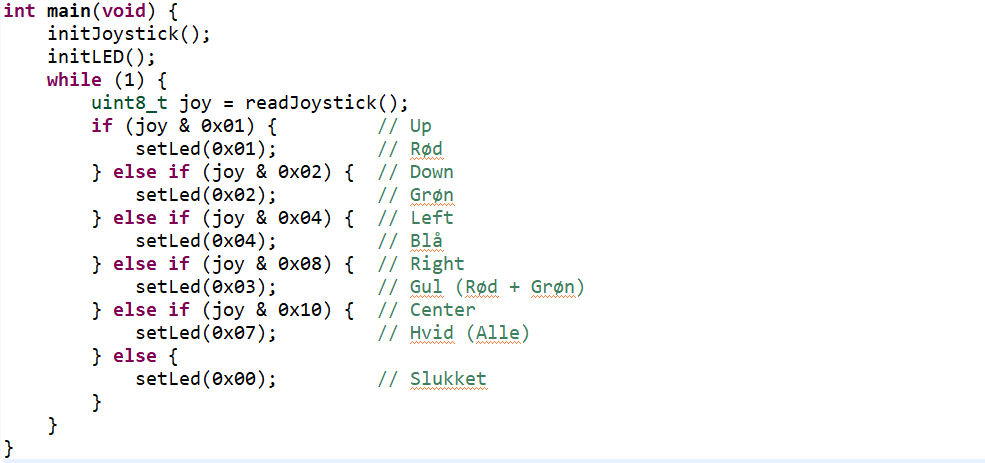
\includegraphics[width=0.7\textwidth]{Picturs/Journal/Led_joy.png}
    \caption{Funktion det styre LED ud fra joystickets position}
\end{figure}

\textbf{Exercise 7.2 - Writing Text on the LCD}

\begin{figure}[h]
    \centering  
    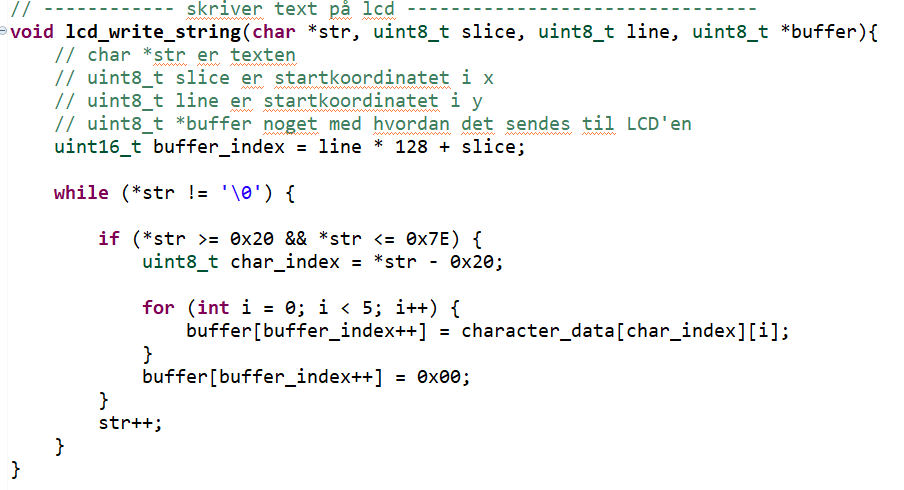
\includegraphics[width=0.7\textwidth]{Picturs/Journal/lcd.png}
    \caption{Funktion til at printe på LCD}
\end{figure}

Vi har ved brug af charset.c filen kunne printe tekst på LCD'en. 

\clearpage
\section*{Dag 6. 12-01-2026}
\vspace{1em}

I dag har vi fået lavet: 
\begin{itemize}
    \setlength{\itemsep}{3pt}
    \setlength{\parskip}{0pt}
    \setlength{\parsep}{0pt}
  \item et udkast til flowdiagram
  \item Box diagram
  \item Valgt kravspecifikationer 
  \item Et gantt chart
\end{itemize}

\textbf{Flowchart}

\begin{figure}[h]
    \centering    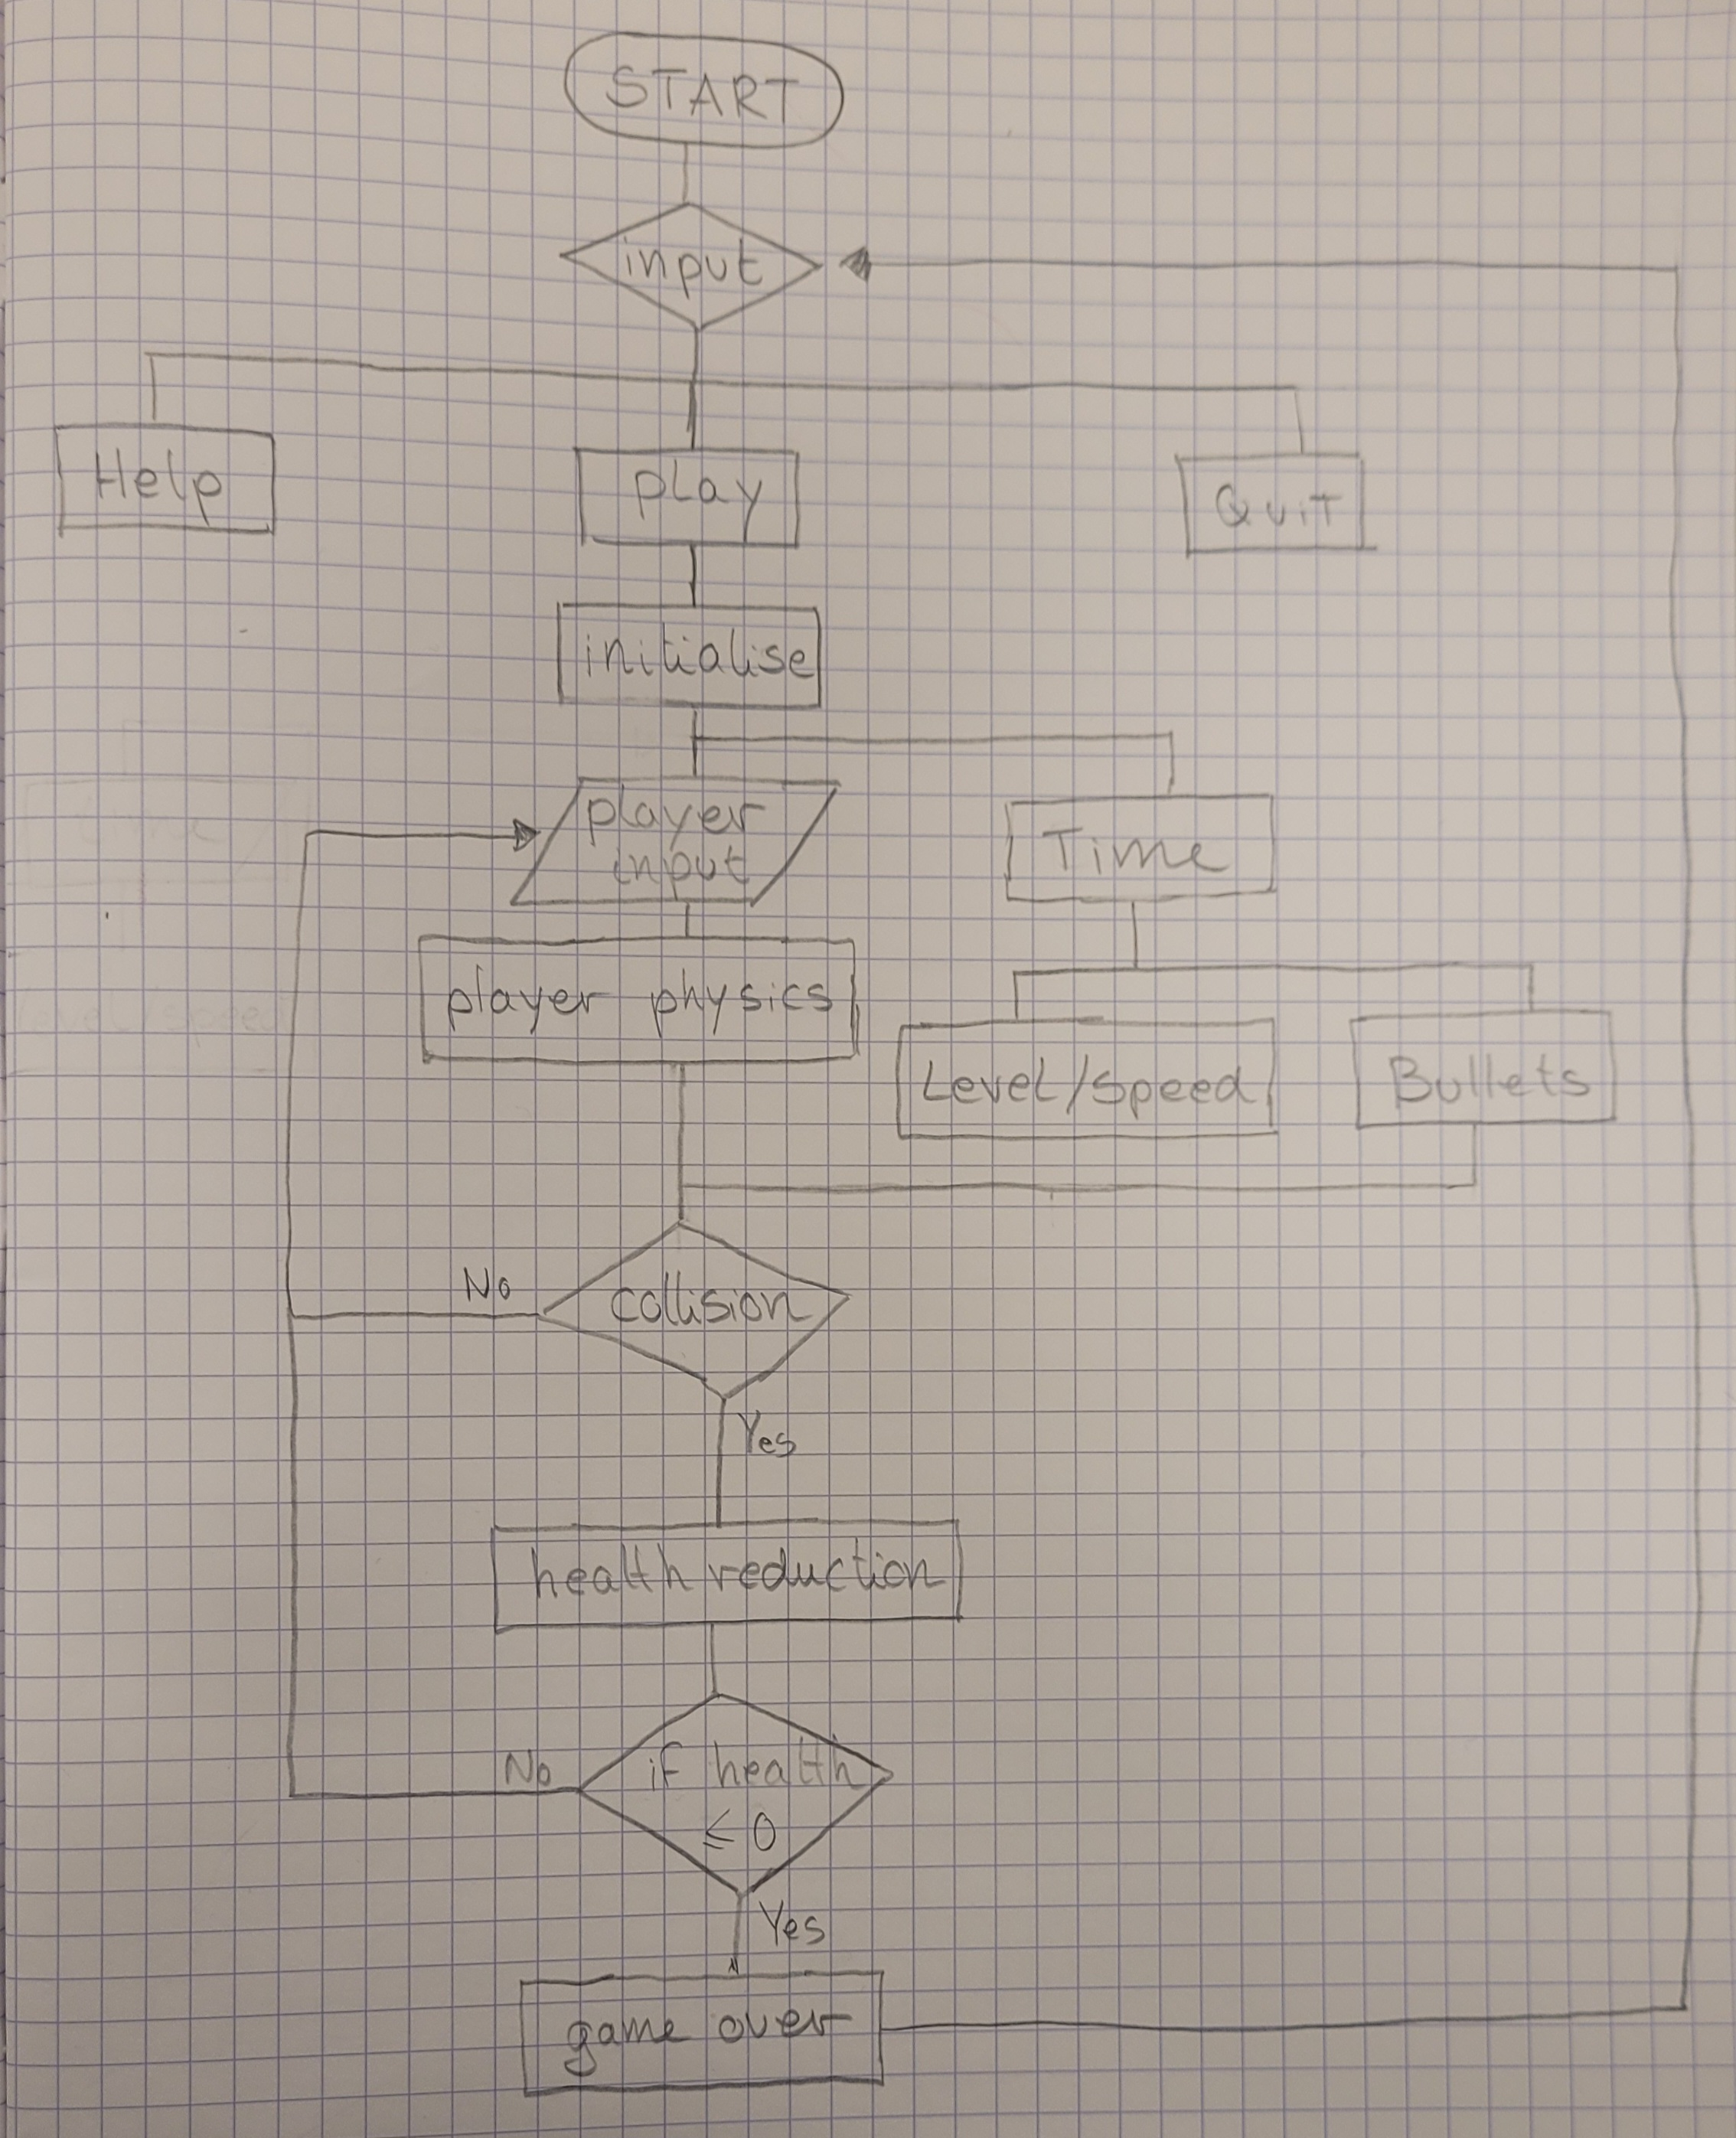
\includegraphics[width=0.9\textwidth]{Picturs/Journal/20260112_160159.jpg}
    \caption{Udkast til Flowdiagram}
\end{figure}

\vspace{4em}

\textbf{Box diagram}

\begin{figure}[h]
    \vspace{-1em}
    \centering  
    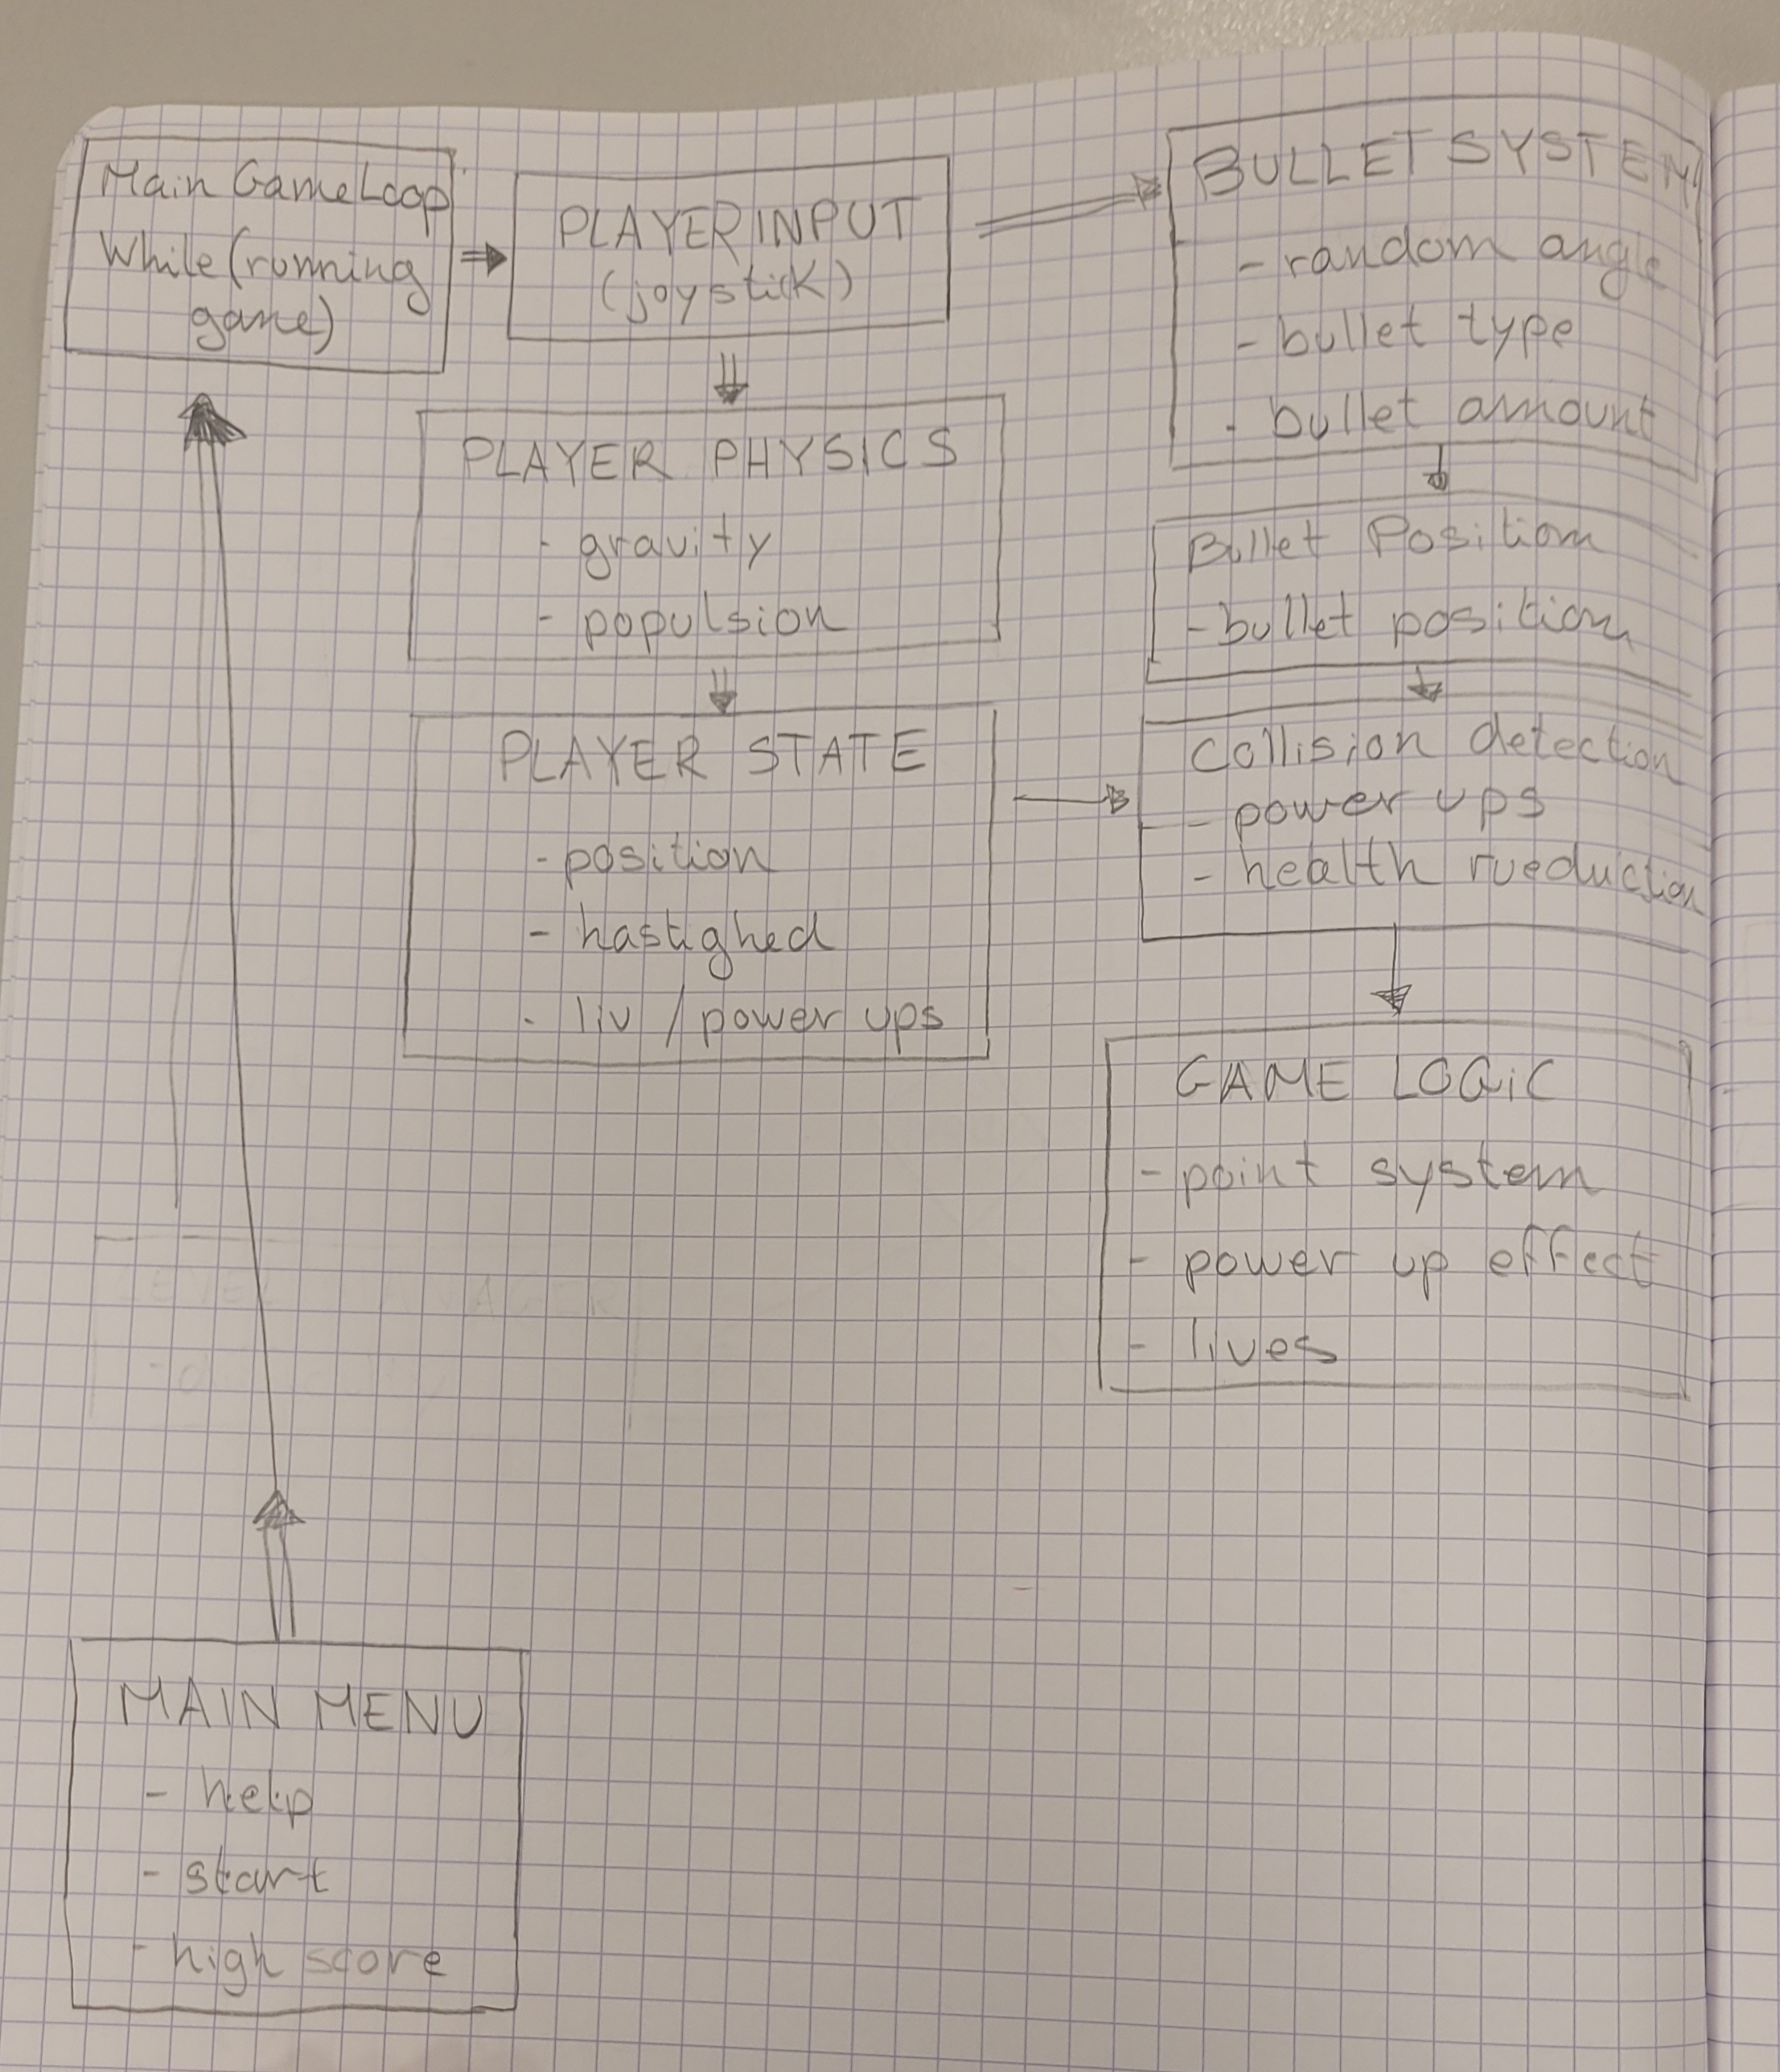
\includegraphics[width=0.7\textwidth]{Picturs/Journal/20260112_160243.jpg}
    \caption{Udkast til block diagram}
    \vspace{-1em}
\end{figure}

\textbf{Gantt chart}

\begin{figure}[h]
    \vspace{-1em}
    \centering    
    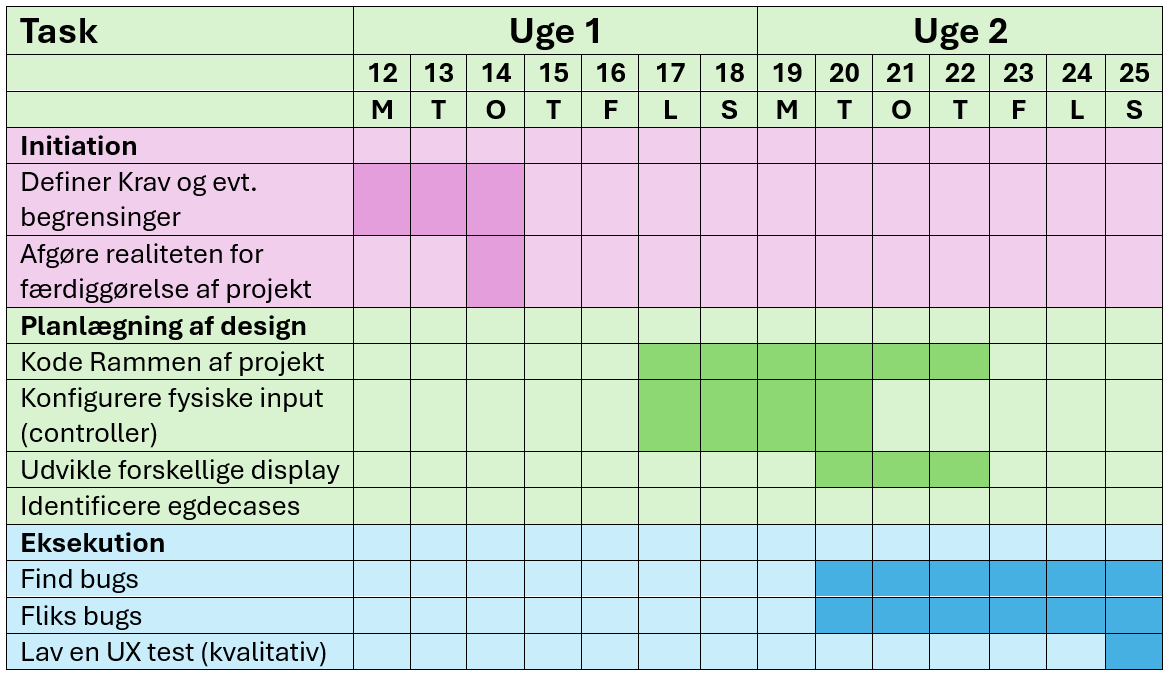
\includegraphics[width=1\textwidth]{Picturs/Journal/gantchart.png}
    \caption{Udkast til Gantt Chart}
    \vspace{-10em}
\end{figure}

\vspace{8em}

\textbf{Valgte kravspesifikationer}

\begin{table}[h!]
\centering
\begin{tabularx}{\textwidth}{|l|X|}
\hline
\textbf{Det vi skal have med} & \textbf{Uddybelse} \\
\hline
Asteroider/planeter med potential felt & no \\
\hline
3+ stages docked spaceships & There are multiple levels (faster, more and different types of bullets) \\
\hline
3+ bullet types + 5+ shot angles & Types of bullets include:
\begin{itemize}[leftmargin=*]
    \item regular bullet: 1 dmg, size: medium (“\%c”,220), speed: medium
    \item bouncing bullet: 1 dmg, size: medium, speed: medium (“\%c”,220) (shot so it hits the wall and bounces)
    \item cannon ball: 2 dmg, size: large 2*(“\%c”,219), speed: slow
    \item sniper bullet: 3 dmg, size: small (“\%c”,254), speed: fast (maybe targeted at player position?)
\end{itemize} \\
\hline
Power-ups & powerups including healing, point multiplier for a time period, some sort of forcefield (outward acceleration or deflection of bullets) \\
\hline
Number of points & point i forhold til tid \\
\hline
Multiple lives & x antal liv som du mister indtil antal liv er x $\leq 0$, og du dør \\
\hline
Menu & 
\begin{itemize}[leftmargin=*]
    \item Help button
    \item Play button
    \item High score
    \item Level (sværhedsgrad)
\end{itemize}
Selected button indikeres af anti characters på given button \\
\hline
Help screen & controls, how to play \\
\hline
Boss key & Brings up a menu displaying the buttons: resume, main menu, help \\
\hline
Random delta-angle & den vinkel “fjenden” skyder med \\
\hline
Multiple bullet & dem som “fjenden” skyder med / meteore \\
\hline
Score / high score & 
\begin{itemize}[leftmargin=*]
    \item displays på LCD
    \item øges med til og evt. powerups
\end{itemize} \\
\hline
Game controlled by 30010 joystick & 
\begin{itemize}[leftmargin=*]
    \item klik: så længe du holder den nede flyver du op
    \item up/down/left/right: bruges måske i menuen
\end{itemize} \\
\hline
Show info on RGB LED &
\begin{itemize}[leftmargin=*]
    \item spil slukket: ingen lys
    \item spil tændt - ikke aktivt: hvid
    \item mens du spiller: grøn
    \item mister et liv: blinker kort i rød
    \item død: rød
\end{itemize} \\
\hline
Partial/full game on the LCD &
\begin{itemize}[leftmargin=*]
    \item displayer løbende score
    \item display af highscore
    \item display af antal liv
\end{itemize}
\end{tabularx}
\end{table}


\clearpage
\section{Full code}
\label{sec:fullcode}

Nedenunder er alle filerne til det komplete program.

\texttt{adc\_buttons.h}
\begin{lstlisting}
    #ifndef ADC_H_
#define ADC_H_

#include <stdint.h>
#include "stm32f30x_conf.h"

// Initialiserer ADC og GPIO
void init_adcbuttons(void);

// Læser ADC-værdi (0–4095) fra valgt kanal (1 eller 2)
uint16_t read_adcbuttons(uint8_t channel);

uint8_t sw1_pressed(void);

// Læser ADC og printer værdi
void update_display_with_adcbuttons(void);

#endif /* ADC_H_ */
\end{lstlisting}

\textbf{adc.h}
\begin{lstlisting}
    #ifndef ADC_H_
#define ADC_H_

#include <stdint.h>
#include "stm32f30x_conf.h"
#include "game_state.h"


// Initialiserer ADC og GPIO
void init_adc(void);

// Læser ADC-værdi (0–4095) fra valgt kanal 8 og 9 (pins CP2 CP3) 
uint16_t read_adc(uint8_t channel);

// Behandler ADC-værdier
void read_joystick_adc(GameContext *ctx);

// Læser ADC og printer værdi
void update_display_with_adc(void);


#endif /* ADC_H_ */
\end{lstlisting}

\texttt{Ascii.h}
\begin{lstlisting}
    #ifndef ASCII_H_
#define ASCII_H_

#include "30010_io.h"
#include "Physics.h"
#include "bullets.h"
#include "game_state.h"

// ansi codes
#define gotoxy(X,Y) printf("\x1B[%d;%dH",(int)(Y),(int)(X))
#define clear() printf("\x1B[2J")
#define hide_cursor() printf("\x1B[?251")

#define BG_DOT "\033[90m%c\033[0m"

// 8.8 Coordinate definitions
#define DISPLAY_HEIGHT  ((uint16_t)0x20)  // 32
#define DISPLAY_WIDTH   ((uint16_t)0x64)  // 100

#define X_COORDINATE    (DISPLAY_WIDTH << 8)
#define Y_COORDINATE    (DISPLAY_HEIGHT << 8)

#define Y_MIN    (1 << 8)
#define Y_MAX    ((DISPLAY_HEIGHT-2) << 8)

#define X_MIN    (1 << 8)
#define X_MAX    ((DISPLAY_WIDTH-2) << 8)

// Alien sprite definition
#define ALIEN_WIDTH   4

// Alien height definitions
#define ALIEN_HEIGHT_LVL_1   3
#define ALIEN_HEIGHT_LVL_2   4
#define ALIEN_HEIGHT_LVL_3   5

// Bullet sizes
#define BULLET_SMALL_HEIGHT   1
#define BULLET_SMALL_WIDTH   2
#define BULLET_MEDIUM_HEIGHT   1
#define BULLET_MEDIUM_WIDTH   3
#define BULLET_LARGE_HEIGHT   3
#define BULLET_LARGE_WIDTH   3

// Powerup sizes
#define POWERUP_WIDTH   5
#define POWERUP_HEIGHT   5

void borders(void);
void game_borders();
void bgcolor(uint8_t background);
void drawSaturn(void);
void drawAlien(player *p, GameContext *ctx);
void drawBullet(Bullet *b);
void eraseAlien(player *p, GameContext *ctx);
void drawPowerup(player *p);
void erasePowerup(player *p);
void print_level(GameContext *ctx);
void print_score(player *p);
void print_hp(player *p);

#endif /* ASCII_H_ */
\end{lstlisting}

\texttt{bullets.h}
\begin{lstlisting}
    #ifndef BULLETS_H
#define BULLETS_H

#include <stdint.h>

typedef struct GameContext GameContext;  // forward declaration OK

// Bullet definitions
#define MAX_BULLETS 20
#define BULLET_WIDTH 3
#define BULLET_HEIGHT_NORMAL   1
#define BULLET_HEIGHT_CANNON   3


#define BULLET_TYPE_REGULAR    1
#define BULLET_TYPE_BOUNCE     2
#define BULLET_TYPE_CANNON     3

// Bullet struct
typedef struct {
    int x, y;
    int vx, vy;
    int ax, ay;
    int alive;
    int type;  // 0=normal (dies at edge), 1=bouncing (reflects at edge)
    uint8_t max_bullets;
} Bullet;

// Bullet system struct, used for all things to do with the bullet array.
typedef struct {
    Bullet bullets[MAX_BULLETS];
    uint8_t max_bullets;
} BulletSystem;

void bullets_init(BulletSystem *bs);
void spawn_simple_bullet(BulletSystem *bs, GameContext *ctx);
void erase_bullet(BulletSystem *bs);
void update_bullets(GameContext *ctx, BulletSystem *bs);
void draw_bullets(BulletSystem *bs);
void bullets_set_max(GameContext *ctx, BulletSystem *bs);
int bullet_height(const Bullet *b);


#endif
\end{lstlisting}

\texttt{charset.h}
\begin{lstlisting}
    #ifndef _CHARSET_H_
#define _CHARSET_H_

#include <stdint.h>
#include "bsp/30010_io.h"

extern const char character_data[95][5];

// ------------ skriver text på lcd ------------------------
void lcd_write_string(char *str, uint8_t slice, uint8_t line, uint8_t *buffer);

// ------------ skriver specifikt ift palyers status --------
void lcd_text(int a, int b, uint8_t *buffer);

// ------------ opdaterer palyers status --------
void score_update(int high, int score);

#endif /*! _CHARSET_H_ */
\end{lstlisting}

\texttt{game\_state.h}
\begin{lstlisting}
    #ifndef MODE_H
#define MODE_H

#include <stdint.h>

#define GAME_STATE_MENU 0
#define GAME_STATE_PLAY 1
#define GAME_STATE_HELP 2
#define GAME_STATE_GAME_OVER 3
#define GAME_STATE_PAUSE 4

#define MENU_MODE_PLAY 0
#define MENU_MODE_HELP 1
#define MENU_MODE_QUIT 2

// Gamecontext struct, used for various variables that arent connected to the player or bullet
typedef struct GameContext {
    uint8_t game_state; // What state the game is in eg. menu, pause, game over.
    uint8_t menu_mode; // What the cursor is hovering in menu
    uint8_t prev_joystick;
    uint32_t timer_counter;
    uint8_t level;
    uint32_t highscore;
    int16_t joy_ax;// resulting acceleration from joystick
    int16_t joy_ay;
    int16_t joy_x; // joystick positions
    int16_t joy_y;

} GameContext;


void game_state_init(GameContext *ctx); // initialize current game state
void game_state_update(GameContext *ctx, uint8_t joystick); // update current game state
void game_init(GameContext *ctx); // initialize game
void game_loop(GameContext *ctx, uint8_t joystick); // update game

#endif
\end{lstlisting}

\texttt{HAL.h}
\begin{lstlisting}
    #ifndef HAL_H
#define HAL_H

#include "bsp/stm32f30x.h"
#include "bsp/30010_io.h"
#include "Physics.h"
#include "game_state.h"

// Joystick
void joystick_init(void);
void joystickdown_init(void);
uint8_t joystick_center_pressed(void);
uint8_t joystick_down_pressed(void);
uint8_t read_joystick(void);


// Timer
void TIM2_Init(void);
void TIM2_IRQHandler(void);

// Global timer flag, most convenient for the timer flag
extern volatile uint8_t tim2_flag;

// Led
void led_update(player *p);
void led_init();
void set_leds(uint8_t led_state);
void led_trigger(player *p);
#endif
\end{lstlisting}

\texttt{heart.h}
\begin{lstlisting}
    #ifndef HEART_H
#define HEART_H

#include <stdint.h>
#include "Physics.h"

// Tegn et fyldt hjerte: 16 kolonner x 13 rækker
void heart_full(uint8_t x, uint8_t y, uint8_t *buffer);

// Tegn et tomt hjerte: 16 kolonner x 13 rækker
void heart_tom(uint8_t x, uint8_t y, uint8_t *buffer);

// Lives display 0 til 5
void display_lives(player *p, uint8_t *buffer);

// Opdatere lives
void liv_update(player *p);

uint8_t *lcd_get_buffer(void);

#endif /* _HEART_H_ */
\end{lstlisting}

\texttt{help.h}
\begin{lstlisting}
    #ifndef HELP_H_
#define HELP_H_
#include "game_state.h"

void displayHelpScreen();
void help_update(GameContext *ctx, uint8_t joystick);
void game_over_update(GameContext *ctx, uint8_t joystick);
void game_over_init(GameContext *ctx);
void pause_update(GameContext *ctx, uint8_t joystick);
#endif /* HELP_H_ */
\end{lstlisting}

\texttt{menu.h}
\begin{lstlisting}
    #ifndef MENU_H
#define MENU_H
#include "game_state.h"
void display_menu(void);
void menu_update(GameContext *ctx, uint8_t joystick);

#endif /* MENU_H */
\end{lstlisting}

\texttt{pause.h}
\begin{lstlisting}
    #ifndef PAUSE_H
#define PAUSE_H

#include "game_state.h"

void pause_init(GameContext *ctx);
void pause_update(GameContext *ctx);
void pause_check(GameContext *ctx);

#endif // PAUSE_H
\end{lstlisting}

\texttt{Physics.h}
\begin{lstlisting}
    #ifndef PHYSICS_H_
#define PHYSICS_H_

#include "30010_io.h"
#include "game_state.h"
#include "bullets.h"
#include <stdbool.h>
#include <stdint.h>

/* ---------------- POWERUPS ---------------- */

typedef enum {
	POWERUP_NONE = 0,
    POWERUP_HEART = 1,
    POWERUP_FORCEFIELD = 2,
    POWERUP_MULTIPLIER = 3
} PowerupType;

typedef struct {
    int32_t x, y;
    int32_t prev_x, prev_y;
    int32_t vx, vy;
    PowerupType type;
    uint8_t active;     // 1 = on screen, 0 = not present
} Powerup;

/* ---------------- PLAYER ---------------- */

typedef struct player {
    int16_t x, y, vy, ay;
    int16_t score, score_multiplier, highscore;
    int16_t width, height;
    int16_t prev_x, prev_y;
    uint8_t hp;
    uint8_t alien_level;

	// powerup pickups
    Powerup heart_pickup;
    Powerup forcefield_pickup;
    Powerup multiplier_pickup;


	uint16_t forcefield_active; // effect active
	uint16_t multiplier_active; // effect active	
	uint16_t forcefield_timer;
	uint16_t multiplier_timer;

	uint16_t led_timer;

} player;

extern player p;

/* ---------------- FUNCTIONS ---------------- */
// collision detections
bool player_collides_with_bullet(player *p, const Bullet *b);
bool heal_collides_with_player(player *p);
bool multiplier_collides_with_player(player *p);
bool forcefield_collides_with_player(player *p);

void player_init(void);
void update_player(player *p, uint8_t joystick, GameContext *ctx);


#endif /* PHYSICS_H_ */
\end{lstlisting}

\texttt{powerup.h}
\begin{lstlisting}
    #ifndef POWERUP_H_
#define POWERUP_H_
#include "game_state.h"
#include "Physics.h"

void spawn_powerup(player *p, GameContext *ctx);
void powerup_forcefield_init(player *p);
void powerup_forcefield_apply(player *p, Bullet *b); // Forcefield effect
void powerup_score_multiplier_init(player *p); // Multiplier and heal effects are simple enough to be in init
void powerup_heal_player(player *p);

void powerup_effects_update(player *p); // Reduce powerup timer and check if 0

void powerups_Update(GameContext *ctx, player *p); // Physical powerup pickup update


#endif /* POWERUP_H_ */
\end{lstlisting}










\texttt{adc.c}
\begin{lstlisting}
    #include "adc.h"
#include <stdio.h>
#include "game_state.h"
#include "Ascii.h"
#include "30010_io.h"
#include "HAL.h"

// ------------------- aktivere ure / kalibrere ADC -------------
void init_adc(void) {
    // Aktiver clock til Port C og ADC12
    RCC->AHBENR |= RCC_AHBPeriph_GPIOC | RCC_AHBPeriph_ADC12;

    // 2. Konfigurer PC2 og PC3 som analog (ADC)
    GPIOC->MODER &= ~((0x3 << (2 * 2)) | (0x3 << (3 * 2)));
    GPIOC->MODER |=  ((0x3 << (2 * 2)) | (0x3 << (3 * 2)));
    
    // Ingen pull-up/pull-down
    GPIOC->PUPDR &= ~((0x0 << (2 * 2)) | (0x0 << (3 * 2)));

    RCC->CFGR2 &= ~RCC_CFGR2_ADCPRE12; // Clear ADC12 prescaler bits
    RCC->CFGR2 |= RCC_CFGR2_ADCPRE12_DIV6; // Set ADC12 prescaler to 6

    ADC1->CR = 0x00000000; // Clear CR register
    ADC1->CFGR &= 0xFDFFC007; // Clear ADC1 config register
    ADC1->SQR1 &= ~ADC_SQR1_L; // Clear regular sequence register 1

    ADC1->CR |= 0x10000000; // Enable internal voltage regulator
    for (volatile i = 0; i < 1000; i++); // Wait for about 16 microseconds
    
    ADC1->CR |= ADC_CR_ADCAL; // Start ADC1 calibration
    while (!(ADC1->CR & ADC_CR_ADCAL)); // Wait for calibration to finish
    for (volatile int i = 0; i < 100; i++); // Wait for a little while


    ADC1->CR |= ADC_CR_ADEN; // Enable ADC1 (0x01 - Enable, 0x02 - Disable
    while (!(ADC1->ISR & 0x00000001)); // Wait until ready
    


}

// ----------- returnere en værdi mellem 0 og 4095 --------------
uint16_t read_adc(uint8_t abs) {
    ADC_RegularChannelConfig(ADC1, abs, 1, ADC_SampleTime_1Cycles5);
    ADC_StartConversion(ADC1); // Start ADC read

  
    while (ADC_GetFlagStatus(ADC1, ADC_FLAG_EOC) == 0); // Wait for ADC read

    return ADC_GetConversionValue(ADC1);
}

void read_joystick_adc(GameContext *ctx)
{
    static uint8_t channel = 0;

    if (channel == 0) {
        ctx->joy_y = ((int)read_adc(0x08) - 2048);// Effectively convert to biased representation for calculations
        channel = 1;
        ctx->joy_ay = ctx->joy_y;
    } else {
        ctx->joy_x = ((int)read_adc(0x09) - 2048);
        channel = 0;
        ctx->joy_ax = ctx->joy_x;
    }
}


// -------------- print for potentiometer(debugging) ----------------------
void update_display_with_adc(void) {
    uint16_t readjoyupdown = read_adc(ADC_Channel_8); //Read the ADC value fra PC2
    uint16_t readjoyleftright = read_adc(ADC_Channel_9); //Read the ADC value fra PC3

    gotoxy(10,10);
    printf("Pot1: %04d | Pot2: %04d\n", readjoyupdown, readjoyleftright);
}

\end{lstlisting}

\texttt{Ascii.c}
\begin{lstlisting}
    #include "Ascii.h"
#include "30010_io.h"
#include "Physics.h"
#include "game_state.h"
#include "bullets.h"

  // grå tegn i baggrunden

void bgcolor(uint8_t background) {

    printf("\x1B[4%dm", background);
}


//--------------game begin borders-------------
void borders(){

	   hide_cursor();
	   clear();
	   gotoxy(1,1);

	printf("%c", 201);
		for(int i=1; i<(DISPLAY_WIDTH-2); i++){
			printf("%c", 205);
		}
		printf("%c", 187);

		for (int f=1; f<DISPLAY_HEIGHT-2; f++){
			gotoxy(1, f+1);
			printf("%c", 186);
			for (int j=1; j<DISPLAY_WIDTH-2;j++){
				printf(BG_DOT, 250);  // 250 er en prik
			}
			printf("%c", 186);
		}

		gotoxy(1, DISPLAY_HEIGHT-1);
		printf("%c", 200);
				for(int i=1; i<(DISPLAY_WIDTH-2); i++){
					printf("%c", 205);
			}
			printf("%c", 188);
}
// General borders
void game_borders(){
	hide_cursor();
	clear();
	gotoxy(1,1);

	for(int i=1; i<(DISPLAY_WIDTH); i++){
		printf("%c", 205);
	}

	for (int f=1; f<DISPLAY_HEIGHT-2; f++){
		gotoxy(1, f+1);
		for (int j=1; j<DISPLAY_WIDTH;j++){
			printf(BG_DOT, 250);  // 250 er en prik
		}
	}

	gotoxy(1, DISPLAY_HEIGHT-1);
			for(int i=1; i<(DISPLAY_WIDTH); i++){
				printf("%c", 205);
		}
}
// ---------- Saturn drawing(not used) ----------
void drawSaturn()
{
    uint16_t saturn_x = 20;  // hard-coded kolonne start
    uint16_t saturn_y = 8;  // hard-coded række start

    int height = sizeof(saturnSprite) / sizeof(saturnSprite[0]);

    // Saturn med grayscale mapping
    for (int i = 0; i < height; i++) {
        gotoxy(saturn_x, saturn_y + i);
        for (int j = 0; saturnSprite[i][j] != '\0'; j++) {
            char c = saturnSprite[i][j];

            if (c == '.')
                printf(BG_DOT, 250);           // background gray dot
            else if (c == ':' || c == '-')
                printf(BG_DOT, 248);           // slightly brighter
            else if (c == '+' || c == '=')
                printf(BG_DOT, 246);           // medium gray
            else if (c == '*')
                printf(BG_DOT, 244);           // darker gray
            else if (c == '@' || c == '%')
                printf(BG_DOT, 242);           // darkest gray
            else if (c == '#')
                printf(BG_DOT, 243);           // medium-dark gray
            else
                printf(BG_DOT, 250);           // background
        }
    }
}

// ---------- Alien sprite ----------
void drawAlien(player *p, GameContext *ctx)
{
	uint16_t x = (p->x >> 8);
	uint16_t y = (p->y >> 8);

// Sprite bestemmes afhængigt af level
	static const char level1[ALIEN_HEIGHT_LVL_1][ALIEN_WIDTH +1] = {
	"<@@>",
	"/||\\",
	"/__\\"
	};

	static const char level2[ALIEN_HEIGHT_LVL_2][ALIEN_WIDTH +1] = {
	"<@@>",
	"/||\\",
	"/__\\",
	" /\\ "
	};

	static const char level3[ALIEN_HEIGHT_LVL_3][ALIEN_WIDTH +1] = {
	"<@@>",
	"/||\\",
	"/__\\",
	" /\\ ",
	" || "
	};

	const char (*sprite)[ALIEN_WIDTH +1];
	int height;
	sprite = NULL;

	switch(ctx->level){
	case 1: // level 1
		sprite = level1;
		height = ALIEN_HEIGHT_LVL_1;
		break;
	case 2: // level 2
		sprite = level2;
		height = ALIEN_HEIGHT_LVL_2;
		break;
	case 3: // level 3
		sprite = level3;
		height = ALIEN_HEIGHT_LVL_3;
		break;

	}

	for (int i = 0; i < height; i++) {
		gotoxy(x, y + i);
		printf("%s", sprite[i]);
	}
}

void eraseAlien(player *p, GameContext *ctx)
{
    int height;

    switch(ctx->level){
    case 1: height = ALIEN_HEIGHT_LVL_1; break;
    case 2: height = ALIEN_HEIGHT_LVL_2; break;
    case 3: height = ALIEN_HEIGHT_LVL_3; break;
    default: height = ALIEN_HEIGHT_LVL_1;
    }

    for (int i=0; i<height; i++) {
        gotoxy((p->prev_x)>>8, (p->prev_y>>8)+i);
        for (int j=0; j<ALIEN_WIDTH; j++) {
            printf(BG_DOT, 250);
            
        }
    }
	p->prev_y = p->y;
}

// ---------- Bullet drawing ----------
void drawBullet(Bullet *b)
{
	// x og y position af øvre venstre hjørne af bullet. Bullet tegnes som læst herfra
	uint16_t x = (b->x >> 8);
	uint16_t y = (b->y >> 8);

	int height = bullet_height(b);

	for(int i=0; i<height; i++){
		gotoxy(x, y+i);
		switch(b->type){
		case 1: printf("---"); break; //regular
		case 2: printf("==="); break; // bouncing
		case 3: printf("OOO"); break; // cannonball
		case 4: printf("**"); break; // sniper(not used)
		}
	}
	if (b->type == 3) {
		height = 3;
	}
}

void drawPowerup(player *p)
{
	// Powerup sprites
	struct { Powerup *pu; const char sprite[POWERUP_HEIGHT][POWERUP_WIDTH+1]; } powerups[] = {
	{ &p->heart_pickup, {
            " *** ",
			"*   *", 
			"*<3 *", 
			"*   *", 
			" *** "
        }},
        { &p->forcefield_pickup, {
            " *** ", 
			"*   *", 
			"*[ ]*", 
			"*   *", 
			" *** "
        }},
        { &p->multiplier_pickup, {
            " *** ", 
			"*\\ /*", 
			"* X *", 
			"*/ \\*", 
			" *** "
        }}
    };

   for (int k = 0; k < 3; k++) {
        Powerup *pu = powerups[k].pu;
        if (!pu->active) continue;

        for (int i = 0; i < POWERUP_HEIGHT; i++) {
            gotoxy(pu->x >> 8, (pu->y >> 8) + i);
            for (int j = 0; j < POWERUP_WIDTH; j++) {
                char c = powerups[k].sprite[i][j];
                printf("%c", c);
            }
        }
    }
}


void erasePowerup(player *p)
{
    Powerup *pickups[] = { &p->heart_pickup, &p->forcefield_pickup, &p->multiplier_pickup }; //powerup array

    for (int k = 0; k < 3; k++) {
        Powerup *pu = pickups[k];
        if (!pu->active) continue;

        for (int i = 0; i < POWERUP_HEIGHT; i++) {
            gotoxy((pu->prev_x >> 8), (pu->prev_y >> 8) + i);
            for (int j = 0; j < POWERUP_WIDTH; j++) {
                printf(BG_DOT, 250);
            }
        }

        // Update prev position after erase
        pu->prev_x = pu->x;
        pu->prev_y = pu->y;
    }
}


//--------------print level--------------
void print_level(GameContext *ctx){
	gotoxy(DISPLAY_WIDTH - 15, 1);
	printf("Level: %d", ctx->level);
}
//-------------print score---------------
void print_score(player *p){
	gotoxy(2, 1);
	printf("Score: %d  Highscore: %d", p->score, p->highscore);
}
//--------------print hp-----------------
void print_hp(player *p){
	gotoxy(40, 1);
	printf("HP: %d  ", p->hp);
}
\end{lstlisting}

\texttt{bullets.c}
\begin{lstlisting}
    #include "Ascii.h"
#include "HAL.h"
#include "bsp/30010_io.h"
#include "bullets.h"
#include <stdlib.h>
#include "help.h"
#include "game_state.h"
#include "adc.h"



void bullets_set_max(GameContext *ctx, BulletSystem *bs)
{
    switch (ctx->level) {
        case 1: bs->max_bullets = 10; break;
        case 2: bs->max_bullets = 15; break;
        case 3: bs->max_bullets = 20; break;
    }
}

// Initialize bullet system
void bullets_init(BulletSystem *bs){
    for(int i = 0; i < bs->max_bullets; i++){
        bs->bullets[i].alive = 0;
        bs->bullets[i].x = 0;
        bs->bullets[i].y = 0;
        bs->bullets[i].vx = 0;
        bs->bullets[i].vy = 0;
        bs->bullets[i].ax = 0;
        bs->bullets[i].ay = 0;
        bs->bullets[i].type = 1;  // Default to type 1 (regular)
    }
}

void spawn_simple_bullet(BulletSystem *bs, GameContext *ctx)
{
    int alive_count = 0;

    // Count alive bullets
    for (int i = 0; i < MAX_BULLETS; i++) {
        if (bs->bullets[i].alive)
            alive_count++;
    }

    // Respect max bullets for current level
    if (alive_count >= bs->max_bullets)
        return;

    // Find ONE free slot and spawn ONE bullet
    for (int i = 0; i < MAX_BULLETS; i++) {
        if (!bs->bullets[i].alive) {
            Bullet *b = &bs->bullets[i];

            b->alive = 1;

            // Spawn position (right side)
            b->x = (DISPLAY_WIDTH - 3) << 8;
            b->y = (2 + rand() % (DISPLAY_HEIGHT - 4)) << 8;


 
             //Random angle (-30° to +30°)
            int angle = (rand() % 61) - 30;

            // Fixed-point velocity
            if (b->type == BULLET_TYPE_CANNON) {
            b->vx = -96;          // slower than regular
            } else {
            b->vx = -160;
            }
            b->vy = (b->vx * angle) / 60;

            read_joystick_adc(ctx);
            // scale to fixed-point acceleration
            b->ax = (ctx->joy_ax >> 9);   
            b->ay = -1*(ctx->joy_ay >> 10);

        // bullet type scales with level
        switch (ctx->level) {
            case 1:
                b->type = 1; // only regular
                break;
        
            case 2: {
                int r = rand() % 10;
                b->type = (r < 3) ? 2 : 1; // 30% bouncing
                break;
            }
        
            case 3: {
                int r = rand() % 10;
                if (r < 2)
                    b->type = 3;      // 20% cannonball
                else if (r < 5)
                    b->type = 2;      // 30% bouncing
                else
                    b->type = 1;      // 50% regular
                break;
            }
        }


            break; // IMPORTANT: only spawn one bullet
        }
    }
}



void erase_bullet(BulletSystem *bs){
    for(int i=0;i<bs->max_bullets;i++){
        if(bs->bullets[i].alive){
            int x = bs->bullets[i].x >> 8;
            int y = bs->bullets[i].y >> 8;
            
            // Erase based on bullet type
            if(bs->bullets[i].type == 3) {
                // Type 3 is 3 lines tall
                for(int line = 0; line < 3; line++) {
                    gotoxy(x, y + line);
                    printf("\033[90m%c%c%c\033[0m", 250, 250, 250);  // 3 spaces for OOO
                }
            } else {
                // Types 1, 2, 4 are 1 line
                gotoxy(x, y);
                if(bs->bullets[i].type == 4) {
                    printf("\033[90m%c%c\033[0m", 250, 250);  // 2 spaces for **
                } else {
                    printf("\033[90m%c%c%c\033[0m", 250, 250, 250);  // 3 spaces for --- or ===
                }
            }
        }
    }
}

void update_bullets(GameContext *ctx, BulletSystem *bs){
    for(int i=0;i<bs->max_bullets;i++){
        if(bs->bullets[i].alive){
            // Update positions
            bs->bullets[i].x += bs->bullets[i].vx;
            bs->bullets[i].y += bs->bullets[i].vy;
            bs->bullets[i].vx += bs->bullets[i].ax;
            bs->bullets[i].vy += bs->bullets[i].ay;

            //-----player bullet collision-----
            if(player_collides_with_bullet(&p, &bs->bullets[i])){
                // Handle collision (e.g., reduce player HP)
            if (bs->bullets[i].type == BULLET_TYPE_CANNON) {
                p.hp -= 2;
            } else {
                p.hp -= 1;
            }



            led_trigger(&p);
            bs->bullets[i].alive = 0;
             // Destroy bullet on hit
                            continue;  // Skip further processing for this bullet
            }


            int screen_x = bs->bullets[i].x >> 8;
            int screen_y = bs->bullets[i].y >> 8;

            if(bs->bullets[i].type == 2) {
                // Bouncing bullet - dies at left edge, bounces at other edges
                if(screen_x < 2) {
                    bs->bullets[i].alive = 0;  // Die at left edge
                } else {
                    // die at right edge
                    if(screen_x > (DISPLAY_WIDTH)) {
                        bs->bullets[i].alive = 0;  // Die at right edge
                    }
            
                    // Bounce off top/bottom edges
                    if(screen_y < 2) {
                        bs->bullets[i].vy = -bs->bullets[i].vy;
                        bs->bullets[i].y = 2 << 8;
                    } else if(screen_y > (DISPLAY_HEIGHT - 2)) {
                        bs->bullets[i].vy = -bs->bullets[i].vy;
                        bs->bullets[i].y = (DISPLAY_HEIGHT - 2) << 8;
                    }
                }
            } 
            else if (bs->bullets[i].type == 1){
                // Normal bullet - dies when it goes off the left edge or top/bottom
                int screen_x = bs->bullets[i].x >> 8;
                int screen_y = bs->bullets[i].y >> 8;
                
                if(screen_x < 2 || screen_y < 2 || screen_y > (DISPLAY_HEIGHT - 2))
                    bs->bullets[i].alive = 0;
            }
            else if(bs->bullets[i].type == 3){
                int screen_x = bs->bullets[i].x >> 8;
                int screen_y = bs->bullets[i].y >> 8;
                
                if(screen_x < 2 || screen_y < 2 || screen_y > (DISPLAY_HEIGHT - 4))
                    bs->bullets[i].alive = 0;
            }

            }
        }
    }




void draw_bullets(BulletSystem *bs){
    for(int i=0;i<bs->max_bullets;i++){
        if(bs->bullets[i].alive){
            gotoxy((int)(bs->bullets[i].x >> 8), (int)(bs->bullets[i].y >> 8));
            drawBullet(&bs->bullets[i]);
        }
    }
}
\end{lstlisting}

\texttt{chartset.c}
\begin{lstlisting}
    
#include "charset.h"
#include <stdint.h>
#include "bsp/30010_io.h"
#include <string.h>

// ------------- Supported ASCII characters -------------------
const char character_data[95][5] = {
  {0x00, 0x00, 0x00, 0x00, 0x00},
  {0x00, 0x5F, 0x5F, 0x00, 0x00},
  {0x00, 0x07, 0x00, 0x07, 0x00},
  {0x14, 0x7F, 0x14, 0x7F, 0x14},
  {0x24, 0x2A, 0x7F, 0x2A, 0x12},
  {0x23, 0x13, 0x08, 0x64, 0x62},
  {0x36, 0x49, 0x55, 0x22, 0x50},
  {0x00, 0x05, 0x03, 0x00, 0x00},
  {0x00, 0x1C, 0x22, 0x41, 0x00},
  {0x00, 0x41, 0x22, 0x1C, 0x00},
  {0x14, 0x08, 0x3E, 0x08, 0x14},
  {0x08, 0x08, 0x3E, 0x08, 0x08},
  {0x00, 0x50, 0x30, 0x00, 0x00},
  {0x08, 0x08, 0x08, 0x08, 0x08},
  {0x00, 0x60, 0x60, 0x00, 0x00},
  {0x20, 0x10, 0x08, 0x04, 0x02},
  {0x3E, 0x51, 0x49, 0x45, 0x3E},
  {0x00, 0x42, 0x7F, 0x40, 0x00},
  {0x42, 0x61, 0x51, 0x49, 0x46},
  {0x22, 0x49, 0x49, 0x49, 0x36},
  {0x18, 0x14, 0x12, 0x7F, 0x10},
  {0x2F, 0x49, 0x49, 0x49, 0x31},
  {0x3E, 0x49, 0x49, 0x49, 0x32},
  {0x03, 0x01, 0x71, 0x09, 0x07},
  {0x36, 0x49, 0x49, 0x49, 0x36},
  {0x26, 0x49, 0x49, 0x49, 0x3E},
  {0x00, 0x36, 0x36, 0x00, 0x00},
  {0x00, 0x56, 0x36, 0x00, 0x00},
  {0x08, 0x14, 0x22, 0x41, 0x00},
  {0x14, 0x14, 0x14, 0x14, 0x14},
  {0x00, 0x41, 0x22, 0x14, 0x08},
  {0x02, 0x01, 0x51, 0x09, 0x06},
  {0x32, 0x49, 0x79, 0x41, 0x3E},
  {0x7C, 0x0A, 0x09, 0x0A, 0x7C},
  {0x7F, 0x49, 0x49, 0x49, 0x36},
  {0x3E, 0x41, 0x41, 0x41, 0x22},
  {0x7F, 0x41, 0x41, 0x41, 0x3E},
  {0x7F, 0x49, 0x49, 0x49, 0x41},
  {0x7F, 0x09, 0x09, 0x09, 0x01},
  {0x3E, 0x41, 0x49, 0x49, 0x7A},
  {0x7F, 0x08, 0x08, 0x08, 0x7F},
  {0x00, 0x41, 0x7F, 0x41, 0x00},
  {0x30, 0x40, 0x40, 0x40, 0x3F},
  {0x7F, 0x08, 0x14, 0x22, 0x41},
  {0x7F, 0x40, 0x40, 0x40, 0x40},
  {0x7F, 0x02, 0x0C, 0x02, 0x7F},
  {0x7F, 0x02, 0x04, 0x08, 0x7F},
  {0x3E, 0x41, 0x41, 0x41, 0x3E},
  {0x7F, 0x09, 0x09, 0x09, 0x06},
  {0x3E, 0x41, 0x51, 0x21, 0x5E},
  {0x7F, 0x09, 0x09, 0x09, 0x76},
  {0x26, 0x49, 0x49, 0x49, 0x32},
  {0x01, 0x01, 0x7F, 0x01, 0x01},
  {0x3F, 0x40, 0x40, 0x40, 0x3F},
  {0x1F, 0x20, 0x40, 0x20, 0x1F},
  {0x3F, 0x40, 0x38, 0x40, 0x3F},
  {0x63, 0x14, 0x08, 0x14, 0x63},
  {0x03, 0x04, 0x78, 0x04, 0x03},
  {0x61, 0x51, 0x49, 0x45, 0x43},
  {0x7F, 0x41, 0x41, 0x00, 0x00},
  {0x02, 0x04, 0x08, 0x10, 0x20},
  {0x00, 0x41, 0x41, 0x7F, 0x00},
  {0x04, 0x02, 0x01, 0x02, 0x04},
  {0x40, 0x40, 0x40, 0x40, 0x40},
  {0x00, 0x01, 0x02, 0x04, 0x00},
  {0x20, 0x54, 0x54, 0x54, 0x78},
  {0x7F, 0x48, 0x44, 0x44, 0x38},
  {0x38, 0x44, 0x44, 0x44, 0x20},
  {0x38, 0x44, 0x44, 0x48, 0x7F},
  {0x38, 0x54, 0x54, 0x54, 0x18},
  {0x08, 0x7E, 0x09, 0x01, 0x02},
  {0x0C, 0x52, 0x52, 0x52, 0x3E},
  {0x7F, 0x08, 0x04, 0x04, 0x78},
  {0x00, 0x44, 0x7D, 0x40, 0x00},
  {0x20, 0x40, 0x44, 0x3D, 0x00},
  {0x7F, 0x10, 0x28, 0x44, 0x00},
  {0x00, 0x41, 0x7F, 0x40, 0x00},
  {0x7C, 0x04, 0x18, 0x04, 0x78},
  {0x7C, 0x08, 0x04, 0x04, 0x78},
  {0x38, 0x44, 0x44, 0x44, 0x38},
  {0x7C, 0x14, 0x14, 0x14, 0x08},
  {0x08, 0x14, 0x14, 0x18, 0x7C},
  {0x7C, 0x08, 0x04, 0x04, 0x08},
  {0x48, 0x54, 0x54, 0x54, 0x20},
  {0x04, 0x3F, 0x44, 0x40, 0x20},
  {0x3C, 0x40, 0x40, 0x20, 0x7C},
  {0x1C, 0x20, 0x40, 0x20, 0x1C},
  {0x3C, 0x40, 0x38, 0x40, 0x3C},
  {0x44, 0x28, 0x10, 0x28, 0x44},
  {0x0C, 0x50, 0x50, 0x50, 0x3C},
  {0x44, 0x64, 0x54, 0x4C, 0x44},
  {0x00, 0x08, 0x36, 0x41, 0x00},
  {0x00, 0x00, 0x7F, 0x00, 0x00},
  {0x00, 0x41, 0x36, 0x08, 0x00},
  {0x08, 0x04, 0x08, 0x10, 0x08}};


// ------------ skriver text på lcd --------------------------------
void lcd_write_string(char *str, uint8_t slice, uint8_t line, uint8_t *buffer){
    // char *str er texten
	// uint8_t slice er startkoordinatet i x
	// uint8_t line er startkoordinatet i y
	// uint8_t *buffer noget med hvordan det sendes til LCD'en
	uint16_t buffer_index = line * 128 + slice;

    while (*str != '\0') {

        if (*str >= 0x20 && *str <= 0x7E) {
            uint8_t char_index = *str - 0x20;

            for (int i = 0; i < 5; i++) {
                buffer[buffer_index++] = character_data[char_index][i];
            }
            buffer[buffer_index++] = 0x00;
        }
        str++;
    }
}

// ------------ skriver specifikt ift palyers status ------------------
void lcd_text(int a, int b, uint8_t *buffer){

    memset(buffer, 0x00, 512);

    // Lav tekstene, inkl. tallet
    char line1[20];
    char line2[20];
    sprintf(line1, "Highscore: %d", a);
    sprintf(line2, "Score: %d", b);

    // Skriv til LCD-buffer
    lcd_write_string(line1, 0, 0, buffer);
    lcd_write_string(line2, 0, 1, buffer);
}


// ------------ updatere palyers status ------------------
void score_update(int high, int score) {
    uint8_t *buffer = lcd_get_buffer();

    memset(buffer, 0x00, 256); // ryd top

    char line1[20], line2[20];
    sprintf(line1, "Highscore: %d", high);
    sprintf(line2, "Score: %d", score);

    lcd_write_string(line1, 0, 0, buffer);
    lcd_write_string(line2, 0, 1, buffer);

    lcd_commit();
}

\end{lstlisting}

\texttt{game\_state.c}
\begin{lstlisting}
    #include "game_state.h"
#include "menu.h"
#include "help.h"
#include "Ascii.h"
#include "HAL.h"
#include "bullets.h"
#include "Physics.h"
#include "charset.h"
#include "heart.h"
#include "powerup.h"
#include "pause.h"
#include "adc.h"

static BulletSystem bullet_system;
// game state initialization dependant on current state
void game_state_init(GameContext *ctx)
{
    clear();

    switch (ctx->game_state) {

        case GAME_STATE_MENU:
            ctx->menu_mode = MENU_MODE_PLAY;   // reset selection
            display_menu();
            break;

        case GAME_STATE_PLAY:
            game_init(ctx);
            break;

        case GAME_STATE_HELP:
            displayHelpScreen();
            break;

        case GAME_STATE_GAME_OVER:
            game_over_init(ctx);
            break;
        case GAME_STATE_PAUSE:
            pause_init(ctx);
            break;
    }
}

 // game state update dependant on current state
void game_state_update(GameContext *ctx, uint8_t joystick)
{
    switch (ctx->game_state) {

        case GAME_STATE_MENU:
            menu_update(ctx, joystick);
            break;

        case GAME_STATE_PLAY:
            game_loop(ctx, joystick);
            break;

        case GAME_STATE_HELP:
            help_update(ctx, joystick);
            break;

        case GAME_STATE_GAME_OVER:
            game_over_update(ctx, joystick);
            break;

        case GAME_STATE_PAUSE:
            pause_update(ctx);
            break;
    }
}


void game_init(GameContext *ctx){
    // initialize game variables here
    ctx->timer_counter = 0;
    ctx->level = 1;
    bullets_init(&bullet_system);
    bullets_set_max(ctx, &bullet_system);
    player_init();   // Initialize player
    game_borders();      // Draw game borders
}
// update game variables
void game_loop(GameContext *ctx, uint8_t joystick){
    pause_check(ctx);
    ctx->timer_counter++;

    if(ctx->timer_counter > 2700){
        ctx->timer_counter = 1800; // reset to avoid overflow
    }
    if(ctx->timer_counter % 900 == 0){
        // Every 30 seconds (30Hz), increase level
        if(ctx->level < 3){
            ctx->level++;
            bullets_set_max(ctx, &bullet_system); // Update max bullets for new level
        }
    }
    //print variables
    print_level(ctx);
    print_score(&p);
    print_hp(&p);
    // update player adjacent stuff
    score_update(p.highscore, p.score);      
    eraseAlien(&p, ctx);
    update_player(&p, joystick, ctx);
    drawAlien(&p, ctx);
    // update powerups
    spawn_powerup(&p, ctx);
    powerups_Update(ctx, &p);
    powerup_effects_update(&p);
    // Update and draw bullets
    erase_bullet(&bullet_system);
    spawn_simple_bullet(&bullet_system, ctx);
    update_bullets(ctx, &bullet_system);
    draw_bullets(&bullet_system);
    // LCD and LED update
    liv_update(&p);
    led_update(&p);
    // If forcefield is active, apply its repulsion to all "living" bullets
if (p.forcefield_active) {
    for (int i = 0; i < bullet_system.max_bullets; i++) {
        Bullet *b = &bullet_system.bullets[i];
        if (b->alive) {
            powerup_forcefield_apply(&p, b);
        }
    }
}
    // check for player hp = 0, is so = game over
if (p.hp <= 0) {
        ctx->game_state = GAME_STATE_GAME_OVER;
        game_state_init(ctx);
    }
}
\end{lstlisting}

\texttt{HAL.c}
\begin{lstlisting}
    #include "HAL.h"
#include "Physics.h"
#include "game_state.h"
#include "Ascii.h"

// LED pins
#define LED1_PIN   4   // PB4
#define LED2_PIN   7   // PC7

// LED timer max
#define LED_BLINK_DURATION 15  // ticks (~0.5 sec at 30Hz)
//-----------------------------------Joystick stuff start------------------------------------------

void joystick_init(void)
{
    RCC->AHBENR |= RCC_AHBPeriph_GPIOB;
    GPIOB->MODER &= ~(0x3 << (5 * 2));   // PB5 input
    GPIOB->PUPDR &= ~(0x3 << (5 * 2));
    GPIOB->PUPDR |=  (0x2 << (5 * 2));   // pull-down
}

void joystickdown_init(void)
{
    RCC->AHBENR |= RCC_AHBPeriph_GPIOB;
    GPIOB->MODER &= ~(0x3 << (0 * 2));   // PB0 input
    GPIOB->PUPDR &= ~(0x3 << (0 * 2));
    GPIOB->PUPDR |=  (0x2 << (0 * 2));   // pull-down
}

uint8_t joystick_center_pressed(void)
{
    return (GPIOB->IDR & (1 << 5)) ? 1 : 0;
}

uint8_t read_joystick(void){
	uint8_t val = 0;
	val |= ((GPIOB->IDR & (0x0001 << 5)) ? 1 : 0); // center
	val |= ((GPIOB->IDR & (0x0001 << 0)) ? 2 : 0); // down
	return val;}
	//-----------------------------------Joystick stuff end------------------------------------------
	//-----------------------------------timer stuff start------------------------------------------

	volatile uint8_t tim2_flag = 0;
	// TIM2 init: 30 Hz interrupt
	void TIM2_Init(void)
	{
	    RCC->APB1ENR |= 0x00000001; // TIM2 clock enable
	    TIM2->PSC = 6399;           // prescaler
	    TIM2->ARR = 332;            // auto-reload
	    TIM2->CNT = 0x0000;         // clear counter
	    TIM2->DIER = 0x0001;        // enable update interrupt
	    TIM2->CR1 = 0x0001;         // enable timer

	    NVIC->ISER[0] = 0x10000000; // enable TIM2 IRQ
	    NVIC->IP[28] = 0x10;        // priority 1
	}

	// TIM2 interrupt handler

	void TIM2_IRQHandler(void)
	{
	    if (TIM2->SR & 0x0001) // UIF flag
	    {
	        TIM2->SR &= ~0x0001; // clear flag
	        tim2_flag = 1;
	    }
	} 

	//-----------------------------------timer stuff end------------------------------------------
	//--------------------------LED stuff start--------------------------------------------
	void led_init(void)
{
    // Enable GPIO clocks
    RCC->AHBENR |= RCC_AHBPeriph_GPIOB | RCC_AHBPeriph_GPIOC;

    // ---- PB4 (LED1) ----
    GPIOB->MODER &= ~(0x3 << (LED1_PIN * 2));  // clear mode
    GPIOB->MODER |=  (0x1 << (LED1_PIN * 2));  // output
    GPIOB->OTYPER &= ~(1 << (LED1_PIN * 1));         // push-pull
    GPIOB->OSPEEDR &= ~(0x3 << (LED1_PIN*2));
    GPIOB->OSPEEDR |=  (0x2 << (LED1_PIN*2));  // medium speed

    // ---- PC7 (LED2) ----
    GPIOC->MODER &= ~(0x3 << (LED2_PIN * 2));  // clear mode
    GPIOC->MODER |=  (0x1 << (LED2_PIN * 2));  // output
    GPIOC->OTYPER &= ~(1 << LED2_PIN);         // push-pull
    GPIOC->OSPEEDR &= ~(0x3 << (LED2_PIN*2));
    GPIOC->OSPEEDR |=  (0x2 << (LED2_PIN*2));  // medium speed

    // Turn off LEDs initially
    GPIOB->ODR &= ~(1 << LED1_PIN);
    GPIOC->ODR &= ~(1 << LED2_PIN);
}
	// Set LED states: bit0 = LED1, bit1 = LED2
void set_leds(uint8_t state)
{
    if (state & 0x01)
        GPIOB->ODR |= (1 << LED1_PIN); //set green
	else 
			GPIOB->ODR &= ~(1 << LED1_PIN); //clear green
    
    if (state & 0x02)
        GPIOC->ODR |= (1 << LED2_PIN); // set red
    else
	        GPIOC->ODR &= ~(1 << LED2_PIN); // clear red


}


// Trigger LED blink
void led_trigger(player *p)
{	

    p->led_timer = LED_BLINK_DURATION; // reset timer
}

void led_update(player *p)
{
    if(p->led_timer > 0){
		set_leds(0x2);    // LED red
        p->led_timer--;
    } else {
        set_leds(0x1);    // LED green
    }
}

//--------------------------LED stuff end--------------------------------------------

\end{lstlisting}

\texttt{heart.c}
\begin{lstlisting}
    #include "heart.h"
#include "bsp/30010_io.h"
#include <stdint.h>
#include <string.h>
#include <stdio.h>
#include "Physics.h"

// ---------------- LCD manager -----------------
uint8_t lcd_buffer[512];
static uint8_t lcd_initialized = 0;

void lcd_manager_init(void) {
    if (!lcd_initialized) {
        lcd_init();
        memset(lcd_buffer, 0x00, 512);
        lcd_initialized = 1;
    }
}

uint8_t *lcd_get_buffer(void) {
    lcd_manager_init();
    return lcd_buffer;
}

void lcd_commit(void) {
    lcd_push_buffer(lcd_buffer);
}
// ------------ Hjerte Full: 16 kolonner x 13 rækker ------------------
const uint16_t full_heart_data[13] = {
    0x1E3C, 0x3F7E, 0x7FFF, 0x7FFF,
    0x7FFF, 0x7FFF, 0x3FFE, 0x1FFC,
    0x0FF8, 0x07F0, 0x03E0, 0x01C0,
    0x0080
};

// ------------- Hjerte Tom: 16 kolonner x 13 rækker ------------------
const uint16_t tom_heart_data[13] = {
    0x1E3C, 0x2142, 0x4081, 0x4001,
    0x4001, 0x4001, 0x2002, 0x1004,
    0x0808, 0x0410, 0x0220, 0x0140,
    0x0080
};

// --------------- Slet hjerte område -------------------------------
void heart_clear(uint8_t x, uint8_t y, uint8_t *buffer) {
    for (int row = 0; row < 13; row++) {
        for (int col = 0; col < 16; col++) {
            uint8_t pixel_x = x + col;
            uint8_t pixel_y = y + row;

            if (pixel_x >= 128 || pixel_y >= 32) continue;

            uint16_t byte_index = (pixel_y / 8) * 128 + pixel_x;
            uint8_t bit = pixel_y % 8;

            buffer[byte_index] &= ~(1 << bit);  // Clear pixel
        }
    }
}

// --------------- Tegn fyldt hjerte -------------------------------
void heart_full(uint8_t x, uint8_t y, uint8_t *buffer) {
    heart_clear(x, y, buffer);  // Clear area first
    
    for (int row = 0; row < 13; row++) {
        uint16_t row_data = full_heart_data[row];

        for (int col = 0; col < 16; col++) {
            if (row_data & (1 << (15 - col))) {
                uint8_t pixel_x = x + col;
                uint8_t pixel_y = y + row;

                if (pixel_x >= 128 || pixel_y >= 32) continue;

                uint16_t byte_index = (pixel_y / 8) * 128 + pixel_x;
                uint8_t bit = pixel_y % 8;

                buffer[byte_index] |= (1 << bit);
            }
        }
    }
}

// ------------------ Tegn tomt hjerte ---------------------------
void heart_tom(uint8_t x, uint8_t y, uint8_t *buffer) {
    heart_clear(x, y, buffer);  // Clear area first
    
    for (int row = 0; row < 13; row++) {
        uint16_t row_data = tom_heart_data[row];

        for (int col = 0; col < 16; col++) {
            if (row_data & (1 << (15 - col))) {
                uint8_t pixel_x = x + col;
                uint8_t pixel_y = y + row;

                if (pixel_x >= 128 || pixel_y >= 32) continue;

                uint16_t byte_index = (pixel_y / 8) * 128 + pixel_x;
                uint8_t bit = pixel_y % 8;

                buffer[byte_index] |= (1 << bit);
            }
        }
    }
}


// ------------ Koordinater for de 5 hjerter (y = lodret, x = vandret) -------------- 
static const uint8_t heart_x[5] = {16, 36, 56, 76, 96}; // vandret med 20 pixels mellemrum
static const uint8_t heart_y[5] = {19, 19, 19, 19, 19}; // lodret samme linje

// ------------- display for de 5 hjærter ---------------------------------------------
void display_lives(player *p, uint8_t *buffer) {
    if (p->hp > 5) p->hp = 5; // begræns til max 5

    for (int i = 0; i < 5; i++) {
        if (i < p->hp) {
            heart_full(heart_x[i], heart_y[i], buffer); // fyldt hjerte
        } else {
            heart_tom(heart_x[i], heart_y[i], buffer);  // tomt hjerte
        }
    }
}

void liv_update(player *p) {
    uint8_t *buffer = lcd_get_buffer();

    display_lives(p, buffer);
    lcd_commit();
}
\end{lstlisting}

\texttt{helpgameoverpause.c}
\begin{lstlisting}
    #include "bsp/30010_io.h"
#include "HAL.h"
#include "Physics.h"
#include "menu.h"
#include "help.h"
#include "Ascii.h"
#include "game_state.h"
#include "charset.h"
#include <stdio.h>
#include "pause.h"


void displayHelpScreen() {
 
           borders();
            // Tegn kanter

            gotoxy(6, 3);{
                printf("HELP - How to play");
            }
            gotoxy(6, 4);{
                printf("Explore a mysterious planet in an endless runner.");
            }
            gotoxy(6, 5);{
                printf("Move up with button held down, otherwise fall down.");
            }
            gotoxy(6, 6);{
                printf("An opposing player can control the initial acceleration of bullets.");
            }
            gotoxy(6, 7);{
                printf("Avoid projectiles. Losing all lives ends the game.");
            }
            gotoxy(6, 9);{
                printf("Controls:");
            }
            gotoxy(8, 10);{
                printf("- Press the non-analog joystick: accelerate upwards");
            }
            gotoxy(8, 11);{
                printf("- Release the non-analog joystick: accelerate downwards");
            }
            gotoxy(8, 12);{
                printf("- Press 'M': pause game");
            }
            gotoxy(8, 13);{
                printf("- Use the analog joystick to control bullet acceleration");
            }
            gotoxy(6, 15);{
                printf("Bullets:");
            }
            gotoxy(8,16); {
                printf("- Regular bullets: damage: -1 HP");
            }
            gotoxy(8,17); {
                printf("- Bouncing bullets: damage: -1 HP");
            }
            gotoxy(8,18);{
                printf("- Cannonball bullets: damage: -2 HP");
            }


            gotoxy(6, 20);{
                printf("Power-ups:");
            }
            gotoxy(8,21); {printf("- Heart: +1 HP");}
            gotoxy(8,22); {printf("- Forcefield: Accelerate bullets away from the alien for 10s");}
            gotoxy(8,23); {printf("- Multiplier: Gain 2X points for 10s");}

            
            gotoxy((DISPLAY_WIDTH >> 1) - 7, DISPLAY_HEIGHT - 2);{
                printf("\x1b[41m");
                printf("[ GO TO MENU ]");
                printf("\x1b[40m");
            }
            gotoxy((DISPLAY_WIDTH >> 1) - 21, DISPLAY_HEIGHT - 4);{
                printf("Press CENTER joystick to return to menu.");
            }

        }
    



void help_update(GameContext *ctx, uint8_t joystick) {
    if (ctx->game_state == GAME_STATE_HELP) {
        uint8_t pressed = joystick & ~ctx->prev_joystick;

        /* CENTER pressed once */
        if (pressed & 0x01) {
            ctx->game_state = GAME_STATE_MENU;
            game_state_init(ctx);
        }

        ctx->prev_joystick = joystick;

    }
}

void game_over_init(GameContext *ctx){
        clear();
        borders();
        gotoxy(50-5,16);{printf("GAME OVER");}
        gotoxy(50-8,18);{printf("your score: %d", p.score);}

        gotoxy((DISPLAY_WIDTH >> 1) - 7, DISPLAY_HEIGHT - 2);{
                   printf("\x1b[41m");
                   printf("[ GO TO MENU ]");
                   printf("\x1b[40m");
               }
               gotoxy((DISPLAY_WIDTH >> 1) - 21, DISPLAY_HEIGHT - 4);{
                   printf("Press CENTER joystick to return to menu.");
               }
        }
    
    

void game_over_update(GameContext *ctx, uint8_t joystick) {
    if (ctx->game_state == GAME_STATE_GAME_OVER) {
        uint8_t pressed = joystick & ~ctx->prev_joystick;

        /* CENTER pressed once */
        if (pressed & 0x01) {
            ctx->game_state = GAME_STATE_MENU;
            game_state_init(ctx);
        }

        ctx->prev_joystick = joystick;

    }
}

void pause_init(GameContext *ctx){
    clear();
    game_borders();
    gotoxy((DISPLAY_WIDTH >> 1) - 3,DISPLAY_HEIGHT >> 1);{printf("PAUSED");}
    gotoxy((DISPLAY_WIDTH >> 1) - 10, DISPLAY_HEIGHT - 4);{
        printf("\x1b[41m");
        printf("[ PRESS B TO RESUME ]");
    }
        gotoxy((DISPLAY_WIDTH >> 1) - 10, DISPLAY_HEIGHT - 2);{
            printf("[ PRESS M TO MENU ]");
        printf("\x1b[40m");
    }
    
}

void pause_update(GameContext *ctx) {
    int ch = uart_get_char();
    if (ch == -1) return;
    
    if (ch == 'b' || ch == 'B') {
        ctx->game_state = GAME_STATE_PLAY;
            gotoxy((DISPLAY_WIDTH >> 1) - 3,DISPLAY_HEIGHT >> 1);
                for (int i; i<6; i++){
        printf(BG_DOT, 250);
        }
    gotoxy((DISPLAY_WIDTH >> 1) - 10, DISPLAY_HEIGHT - 4);
        for (int i; i<21; i++){
        printf(BG_DOT, 250);
        }
    
        gotoxy((DISPLAY_WIDTH >> 1) - 10, DISPLAY_HEIGHT - 2);
        for (int i; i<19; i++){
        printf(BG_DOT, 250);
        }
    }

     else if (ch == 'm' || ch == 'M') {
        ctx->game_state = GAME_STATE_MENU;
        game_state_init(ctx);
    }
}



void pause_check(GameContext *ctx)
{
    int ch = uart_get_char();   // NON-blocking

    if (ch == -1)
        return;                // no input = keep running

    if (ctx->game_state == GAME_STATE_PLAY &&
        (ch == 'b' || ch == 'B'))
    {
        ctx->game_state = GAME_STATE_PAUSE;
        game_state_init(ctx);
    
    }
}

\end{lstlisting}

\texttt{main.c}
\begin{lstlisting}
    #include "bsp/stm32f30x_conf.h" // STM32 config
#include "bsp/30010_io.h" // Input/output library for this course
#include "HAL.h"
#include "Ascii.h"
#include "Physics.h"
#include "charset.h"
#include "heart.h"
#include <string.h>
#include "menu.h"
#include "game_state.h"
#include "bullets.h"
#include "adc.h"


int main(){
	//-----------inits start------------------
    uart_init(950000); // Baud rate 950000, compiler didnt like it :( 
	printf("\x1b[?25l"); // Hide terminal cursor
    joystick_init();
    joystickdown_init();
    TIM2_Init();
	led_init();
	init_adc();
	clear();
	GameContext ctx = {
    .game_state = GAME_STATE_MENU,
    .menu_mode  = MENU_MODE_PLAY,
	.prev_joystick = 0,
	.timer_counter = 0,
	.level = 1,
	.highscore = 0,
	};
	uint8_t joystick = 0;
	game_state_init(&ctx);
	//inits end
    	while(1){
			joystick = read_joystick();
    		if (tim2_flag){ //30 Hz timer flag, bruges til main time
    						//player movement, bullet movement, etc.

				game_state_update(&ctx, joystick);
				
    			tim2_flag = 0;
    		}
    	}
} 



// score_update(3, 3475);       // 1. værdig er highscore, 2. værdig er current score (er begger int)
// liv_update(4);               // antal liv (1 til 5)
\end{lstlisting}

\texttt{menu.c}
\begin{lstlisting}
    #include "game_state.h"
#include "Ascii.h"
#include "HAL.h"
#include "Physics.h"
#include "menu.h"
#include "help.h"
#include <stdlib.h>


void display_menu(void){
    int w=DISPLAY_WIDTH,h=DISPLAY_HEIGHT;

       borders();
	
        gotoxy(w/2-4,h/4);
        printf("Rum Reje");
        gotoxy(w/2-15,h/2);
        printf("Press JOYSTICK to PLAY level 1");// 
        gotoxy(w/2-2,h/2+2); 
        bgcolor(1);printf("PLAY");bgcolor(9);
        gotoxy(w/2-2,h/2+4); 
        printf("HELP");
        gotoxy(w/2-2,h/2+6);
        printf("QUIT");
         
      }
 

void menu_update(GameContext *ctx, uint8_t joystick)
{
    uint8_t pressed = joystick & ~ctx->prev_joystick;

    /* DOWN pressed once */
    if (pressed & 0x02) {
        ctx->menu_mode = (ctx->menu_mode + 1) % 3;
    }

    /* CENTER pressed once */
    if (pressed & 0x01) {
        if (ctx->menu_mode == MENU_MODE_PLAY) {
            ctx->game_state = GAME_STATE_PLAY;
            game_state_init(ctx);
        }
        else if (ctx->menu_mode == MENU_MODE_HELP) {
            ctx->game_state = GAME_STATE_HELP;
            game_state_init(ctx);
        }
        else if (ctx->menu_mode == MENU_MODE_QUIT) {
            clear();
            gotoxy((DISPLAY_WIDTH >> 1)-7, 16);
            printf("Exiting game...");
            gotoxy(0, 0);
            printf("\x1b[?25h"); // Show terminal cursor
            exit(0);
        }
    }

    ctx->prev_joystick = joystick;

uint8_t h=DISPLAY_HEIGHT; uint8_t w = DISPLAY_WIDTH;

    /* Draw selection */
    if (ctx->menu_mode == MENU_MODE_PLAY && ctx->game_state == GAME_STATE_MENU) {
        printf("\x1B[%d;%dH\033[41mPLAY\033[0m",(h/2)+2,(w/2)-2);
        printf("\x1B[%d;%dHHELP",(h/2)+4,(w/2)-2);
        printf("\x1B[%d;%dHQUIT",(h/2)+6,(w/2)-2);
    }
    else if (ctx->menu_mode == MENU_MODE_HELP && ctx->game_state == GAME_STATE_MENU) {
        printf("\x1B[%d;%dHPLAY",(h/2)+2,(w/2)-2);
        printf("\x1B[%d;%dH\033[41mHELP\033[0m",(h/2)+4,(w/2)-2);
        printf("\x1B[%d;%dHQUIT",(h/2)+6,(w/2)-2);
    }
    else if (ctx->menu_mode == MENU_MODE_QUIT && ctx->game_state == GAME_STATE_MENU) {
        printf("\x1B[%d;%dHPLAY",(h/2)+2,(w/2)-2);
        printf("\x1B[%d;%dHHELP",(h/2)+4,(w/2)-2);
        printf("\x1B[%d;%dH\033[41mQUIT\033[0m",(h/2)+6,(w/2)-2);
    }

  
}
\end{lstlisting}

\texttt{Physics.c}
\begin{lstlisting}
    #include "Physics.h"
#include "Ascii.h"
#include "HAL.h"
#include "bullets.h"
#include "game_state.h"
#include "stm32f30x_flash.h"
 
//----------------player Physics----------------------
player p; 

void player_init(){
	// movement
	p.x=X_COORDINATE/6;
	p.y=Y_COORDINATE/2;
	p.vy=0;
	p.ay=0;
	p.prev_x=p.x;
	p.prev_y=p.y;

	//general attributes
	p.score=0;
	p.score_multiplier=1;
	p.hp=5;

	//physical attributes
	p.height=ALIEN_HEIGHT_LVL_1;
	p.width=ALIEN_WIDTH;
	
	//powerup effect status
	p.forcefield_active = 0;
	p.multiplier_active = 0;
	p.forcefield_timer = 0;
	p.multiplier_timer = 0;

	//pickup inits
	p.heart_pickup.active = 0;
    p.heart_pickup.x = 0;
    p.heart_pickup.y = 0;
    p.heart_pickup.prev_x = 0;
    p.heart_pickup.prev_y = 0;
    p.heart_pickup.vx = 0;
    p.heart_pickup.vy = 0;
    p.heart_pickup.type = POWERUP_HEART;

	p.forcefield_pickup.active = 0;
    p.forcefield_pickup.x = 0;
    p.forcefield_pickup.y = 0;
    p.forcefield_pickup.prev_x = 0;
    p.forcefield_pickup.prev_y = 0;
    p.forcefield_pickup.vx = 0;
    p.forcefield_pickup.vy = 0;
    p.forcefield_pickup.type = POWERUP_FORCEFIELD;

	p.multiplier_pickup.active = 0;
    p.multiplier_pickup.x = 0;
    p.multiplier_pickup.y = 0;
    p.multiplier_pickup.prev_x = 0;
    p.multiplier_pickup.prev_y = 0;
    p.multiplier_pickup.vx = 0;
    p.multiplier_pickup.vy = 0;
    p.multiplier_pickup.type = POWERUP_MULTIPLIER;

	//led stuff
	p.led_timer = 0;
}

inline int bullet_height(const Bullet *b)
{
    switch (b->type) {
        case 3:  // cannonball
            return BULLET_HEIGHT_CANNON;
        default: // regular, bouncing, sniper, etc.
            return BULLET_HEIGHT_NORMAL;
    }
}


bool player_collides_with_bullet(player *p, const Bullet *b){
	// Define player collision box
	int player_left = p->x >> 8;
	int player_right = player_left + p->width;
	int player_top = p->y >> 8;
	int player_bottom = player_top + p->height;

	// Define bullet collision box
	int bullet_left = b->x >> 8;
	int bullet_right = bullet_left + BULLET_WIDTH;
	int bullet_top = b->y >> 8;
	int bullet_bottom = bullet_top + bullet_height(b);

	// Check for overlap
	if (player_left < bullet_right &&
		player_right > bullet_left &&
		player_top < bullet_bottom &&
		player_bottom > bullet_top) {
		return true;  // Collision detected
	}
	return false;  // No collision
}

bool heal_collides_with_player(player *p) {
	// Define player collision box
	int player_left = p->x >> 8;
	int player_right = player_left + p->width;
	int player_top = p->y >> 8;
	int player_bottom = player_top + p->height;

	// Define heal powerup collision box
	int heal_left = p->heart_pickup.x >> 8;
	int heal_right = heal_left + POWERUP_WIDTH;
	int heal_top = p->heart_pickup.y >> 8;
	int heal_bottom = heal_top + POWERUP_HEIGHT;

	// Check for overlap
	if (player_left < heal_right &&
		player_right > heal_left &&
		player_top < heal_bottom &&
		player_bottom > heal_top) {
		return true;  // Collision detected
	}
	return false;  // No collision
}

bool multiplier_collides_with_player(player *p) {
	// Define player collision box
	int player_left = p->x >> 8;
	int player_right = player_left + p->width;
	int player_top = p->y >> 8;
	int player_bottom = player_top + p->height;

	// Define multiplier powerup collision box
	int mult_left = p->multiplier_pickup.x >> 8;
	int mult_right = mult_left + POWERUP_WIDTH;
	int mult_top = p->multiplier_pickup.y >> 8;
	int mult_bottom = mult_top + POWERUP_HEIGHT;

	// Check for overlap
	if (player_left < mult_right &&
		player_right > mult_left &&
		player_top < mult_bottom &&
		player_bottom > mult_top) {
		return true;  // Collision detected
	}
	return false;  // No collision
}

bool forcefield_collides_with_player(player *p) {
	// Define player collision box
	int player_left = p->x >> 8;
	int player_right = player_left + p->width;
	int player_top = p->y >> 8;
	int player_bottom = player_top + p->height;

	// Define forcefield powerup collision box
	int ff_left = p->forcefield_pickup.x >> 8;
	int ff_right = ff_left + POWERUP_WIDTH;
	int ff_top = p->forcefield_pickup.y >> 8;
	int ff_bottom = ff_top + POWERUP_HEIGHT;

	// Check for overlap
	if (player_left < ff_right &&
		player_right > ff_left &&
		player_top < ff_bottom &&
		player_bottom > ff_top) {
		return true;  // Collision detected
	}
	return false;  // No collision
}

void update_player(player* p, uint8_t joystick, GameContext *ctx){
// -----movement physics-----
	if (joystick & 0x01){
		p->ay = -16; //op
	}
	else if (!(joystick == 0x01)){
		p->ay = 8; //gravity
	}
	// -----score update-----
	p->score += p->score_multiplier;
	
    if (p->score > p->highscore) {
        p->highscore = p->score;
    }
	// -----position update-----
	p->vy += p->ay;
	p->y += p->vy;

	// -----boundary conditions-----
	switch (ctx->level)
	{
	case 1:
		/* code */
	if (p->y < Y_MIN + 256){
		p->y = Y_MIN + 256;
		p->vy = 0;
		
	}
	else if (p->y > Y_MAX - ((ALIEN_HEIGHT_LVL_1 - 1) << 8)){
		p->y = Y_MAX - ((ALIEN_HEIGHT_LVL_1 - 1) << 8);
		p->vy = 0;
	}
		break;
	case 2:
	if (p->y < Y_MIN + 256){
		p->y = Y_MIN + 256;
		p->vy = 0;
	}
	else if (p->y > Y_MAX - ((ALIEN_HEIGHT_LVL_2 - 1) << 8)){
		p->y = Y_MAX - ((ALIEN_HEIGHT_LVL_2 - 1) << 8);
		p->vy = 0;
	
	}
		break;
	case 3:
	if (p->y < Y_MIN + 256){
		p->y = Y_MIN + 256;
		p->vy = 0;
	}
	else if (p->y > Y_MAX - ((ALIEN_HEIGHT_LVL_3 - 1) << 8)){
		p->y = Y_MAX - ((ALIEN_HEIGHT_LVL_3 - 1) << 8);
		p->vy = 0;
	}
		break;
	}
	// -----height update-----
	if (ctx->level == 1){
		p->height = ALIEN_HEIGHT_LVL_1;
		p->width = ALIEN_WIDTH;
	}
	if (ctx->level == 2){
		p->height = ALIEN_HEIGHT_LVL_2;
		p->width = ALIEN_WIDTH;
	}
	else if (ctx->level == 3){
		p->height = ALIEN_HEIGHT_LVL_3;
		p->width = ALIEN_WIDTH;
	}
}


\end{lstlisting}
\texttt{powerup.c}
\begin{lstlisting}
    #include "Physics.h"
#include "bullets.h"
#include "Ascii.h"
#include <math.h>
#include <stdint.h>
#include "game_state.h"
#include <stdbool.h>
#include "powerup.h"

void spawn_powerup(player *p, GameContext *ctx) {
    uint32_t t = ctx->timer_counter;

   if ((t+600) % 900 == 0 && !p->heart_pickup.active) {
        p->heart_pickup.active = 1;
        p->heart_pickup.type = POWERUP_HEART;
        p->heart_pickup.x = DISPLAY_WIDTH << 8;
        p->heart_pickup.y = 5 << 8;
        p->heart_pickup.vx = -128;
        p->heart_pickup.vy = 0;
    }
    

    if ((t+300) % 900 == 0 && !p->forcefield_pickup.active) {
        // spawn forcefield
        p->forcefield_pickup.active = 1;
        p->forcefield_pickup.type = POWERUP_FORCEFIELD;
        p->forcefield_pickup.x = DISPLAY_WIDTH << 8;
        p->forcefield_pickup.y = 12 << 8;
        p->forcefield_pickup.vx = -128;
        p->forcefield_pickup.vy = 0;
    }

    if (t % 900 == 0 && !p->multiplier_pickup.active) {
        // spawn multiplier
        p->multiplier_pickup.active = 1;
        p->multiplier_pickup.type = POWERUP_MULTIPLIER;
        p->multiplier_pickup.x = DISPLAY_WIDTH << 8;
        p->multiplier_pickup.y = 20 << 8;
        p->multiplier_pickup.vx = -128;
        p->multiplier_pickup.vy = 0;
    }
}

void powerup_heal_player(player *p) { //should be called when there is collision with heal powerup
        p->hp += 2; // Heal 2 HP
        if (p->hp > 5) {  // Assuming max HP is 5
            p->hp = 5;
        }
}

void powerup_score_multiplier_init(player *p) { //should be called when there is collision with score multiplier powerup
            p->score_multiplier = 2;  // Double score
            p->multiplier_active = 1;
            p->multiplier_timer = 300;  // Set timer for 300 ticks
    
}


void powerup_forcefield_init(player *p) { //should be called when there is collision with forcefield powerup
            p->forcefield_active = 1;
            p->forcefield_timer = 300;
        
   
}

void powerup_effects_update(player *p) {
    //------multiplier effect update------
    {
    if (p->multiplier_timer > 0) {
        p->multiplier_timer--;
        if (p->multiplier_timer == 0) {
            p->score_multiplier = 1;  // Reset to normal score
            p->multiplier_active = 0;
        }
    }
}
    //------forcefield effect update------
    if (p->forcefield_timer > 0) {
        p->forcefield_timer--;
        if (p->forcefield_timer == 0) {
            p->forcefield_active = 0;
        }
    }
}
void powerup_forcefield_apply(player *p, Bullet *b) {

    int32_t player_center_x = (int32_t)p->x + ((int32_t)p->width << 8);
    int32_t player_center_y = (int32_t)p->y + ((int32_t)p->height << 8);
    int32_t bullet_center_x = (int32_t)b->x + ((int32_t)BULLET_WIDTH << 8);
    int32_t bullet_center_y = (int32_t)b->y + ((int32_t)bullet_height(b) << 8);

    int32_t dx_fixed = bullet_center_x - player_center_x; // fixed 8.8
    int32_t dy_fixed = bullet_center_y - player_center_y; // fixed 8.8

    float dx_pix = dx_fixed / 256.0f;
    float dy_pix = dy_fixed / 256.0f;
    float dist = sqrtf(dx_pix * dx_pix + dy_pix * dy_pix);
    if (dist <= 0.0f) return; // safety

    const float EFFECT_RADIUS = 15; // pixels
    if (dist < EFFECT_RADIUS) {
        float nx = dx_pix / dist;
        float ny = dy_pix / dist;

        // Strength scales with proximity: closer -> stronger push
        // Tweak the constant to get desired gameplay feel
        float strength_pixels = (EFFECT_RADIUS - dist) * 0.005f; // pixels/tick^2

        // Convert to 8.8 fixed point for ax/ay
        int ax_fixed = (int)(nx * strength_pixels * 256.0f);
        int ay_fixed = (int)(ny * strength_pixels * 256.0f);

        // Apply acceleration away from player (add because nx points from player->bullet)
        b->ax += ax_fixed;
        b->ay += ay_fixed;
    } else {
        // Outside effect radius: reset acceleration to 0
        b->ax = 0;
        b->ay = 0;
    }
}


// Updates powerups using random test powerups
// Bevæger sig vandret og bouncer af vægge (hvis vi vil bruge denne funktion)
void powerups_Update(GameContext *ctx, player *p) {
    // Only do anything if the game is in play mode
    

    // --- Erase old powerups ---
    if (p->heart_pickup.active)
        erasePowerup(p);
    if (p->forcefield_pickup.active)
        erasePowerup(p);
    if (p->multiplier_pickup.active)
        erasePowerup(p);


    // --- move ---
 if (p->heart_pickup.active) {
        p->heart_pickup.prev_x = p->heart_pickup.x;
        p->heart_pickup.prev_y = p->heart_pickup.y;
        p->heart_pickup.x += p->heart_pickup.vx;
        p->heart_pickup.y += p->heart_pickup.vy;

        // Deactivate if off screen
        if ((p->heart_pickup.x >> 8) < 0 || (p->heart_pickup.x >> 8) >= DISPLAY_WIDTH ||
        (p->heart_pickup.y >> 8) < 0 || (p->heart_pickup.y >> 8) >= DISPLAY_HEIGHT) {
        p->heart_pickup.active = 0;
    }
    }

    if (p->forcefield_pickup.active) {
        p->forcefield_pickup.prev_x = p->forcefield_pickup.x;
        p->forcefield_pickup.prev_y = p->forcefield_pickup.y;
        p->forcefield_pickup.x += p->forcefield_pickup.vx;
        p->forcefield_pickup.y += p->forcefield_pickup.vy;

        // Deactivate if off screen
    if ((p->forcefield_pickup.x >> 8) < 0 || (p->forcefield_pickup.x >> 8) >= DISPLAY_WIDTH ||
        (p->forcefield_pickup.y >> 8) < 0 || (p->forcefield_pickup.y >> 8) >= DISPLAY_HEIGHT) {
        p->forcefield_pickup.active = 0;
    }
    }

    if (p->multiplier_pickup.active) {
        p->multiplier_pickup.prev_x = p->multiplier_pickup.x;
        p->multiplier_pickup.prev_y = p->multiplier_pickup.y;
        p->multiplier_pickup.x += p->multiplier_pickup.vx;
        p->multiplier_pickup.y += p->multiplier_pickup.vy;

        // Deactivate if off screen
        if ((p->multiplier_pickup.x >> 8) < 0 || (p->multiplier_pickup.x >> 8) >= DISPLAY_WIDTH ||
        (p->multiplier_pickup.y >> 8) < 0 || (p->multiplier_pickup.y >> 8) >= DISPLAY_HEIGHT) {
        p->multiplier_pickup.active = 0;
    }
    }
    //---------collision-----------
     if (p->heart_pickup.active && heal_collides_with_player(p)) {
        p->heart_pickup.active = 0;
        powerup_heal_player(p);
    }

    if (p->multiplier_pickup.active && multiplier_collides_with_player(p)) {
        p->multiplier_pickup.active = 0;
        powerup_score_multiplier_init(p);
    }

    if (p->forcefield_pickup.active && forcefield_collides_with_player(p)) {
        p->forcefield_pickup.active = 0;
        powerup_forcefield_init(p);
    }


    // --- Draw updated powerups ---
    if (p->heart_pickup.active)
        drawPowerup(p);
    if (p->forcefield_pickup.active)
        drawPowerup(p);
    if (p->multiplier_pickup.active)
        drawPowerup(p);

}



\end{lstlisting}
\clearpage
\newgeometry{left=28mm,right=14mm,top=42mm,bottom=14mm}
\thispagestyle{empty}
\pagecolor{frontbackcolor}
\color{white}

\vspace*{\fill}



\begin{tabular}{@{}l}
    Danmarks \\ 
    Tekniske \\ 
    Universitet \\
    \\
    \addressI \\
    \addressII \\
    Tlf. 4525 1700 \\
    \\
    \url{\departmentwebsite}
\end{tabular}



\end{document}